\documentclass[10pt]{reportMaster}

\usepackage[a4paper]{geometry}
\usepackage{amsmath}
\usepackage{amssymb}
\usepackage{amsthm}
\usepackage{graphicx}
\usepackage{float}
\usepackage{hyperref}
\usepackage{enumitem}
\usepackage{subcaption}
\usepackage{placeins}
\usepackage[hang,flushmargin]{footmisc}
\usepackage[backend=biber,sorting=none]{biblatex}

\graphicspath{/images}
\addbibresource{bibliography.bib}
% \hypersetup{hidelinks} % uncomment for hidden links

\DeclareMathOperator*{\argmax}{argmax}
\DeclareMathOperator*{\argmin}{argmin}

\newtheorem{assumption}{Assumption}

\title{Continual Reinforcement Learning for Evolving Games: Learning Across Game Updates in Competitive Pokémon}
\author{Thomas Vroom}

\nameMastersProgramme{Artificial Intelligence}
\committee{Dr. D.J.N.J. Soemers \\ Dr. Ir. K. Driessens}

\begin{document}

% title page
\maketitle

% abstract
%
% Abstract
%
\chapter*{Abstract}
Many modern live-service games receive frequent updates that modify existing game mechanics, intentionally altering the strategic landscape to maintain competitive balance and player engagement.
This poses a major challenge for the development of competitive reinforcement learning agents, whose learned strategies may suddenly be invalidated by these updates.
In place of complete retraining after every update, we investigate whether continual reinforcement learning can facilitate effective knowledge transfer across game versions.
The domain of this research is competitive Pokémon, also known as VGC, a challenging environment that sees natural non-stationarity through its seasonal rulesets.

Our results show that reinforcement learning agents suffer greatly from non-stationarity in VGC, unable to transfer their learned knowledge to different rulesets without further training.
We propose network adjustments aimed at stabilizing the value function, a progressive network architecture, and a tuned training algorithm as potential ways to facilitate better knowledge transfer across rulesets.
Our results show that a combination of our proposed network adjustments and tuned training algorithm improves knowledge transfer across rulesets compared to conventional fine-tuning, while also yielding better generalization to unseen scenarios.
While the progressive architecture exhibits similar improved generalization, it is not able to facilitate better knowledge transfer.

Overall, agents trained with our proposed continual learning methods are not able to consistently outperform agents retrained from scratch in either performance or generalization, indicating that full retraining remains the most effective approach in VGC.
Nevertheless, our proposed methods still improve the outright performance and generalization compared to traditional agents, suggesting that continual learning is still beneficial to reinforcement learning agents in VGC.

% LLM usage disclosure
\begin{NoHyper}
    \renewcommand\thefootnote{}\footnote{\textbf{LLM Usage Disclosure:} A large language model (\textit{GPT5.5-Instant}) was used to draft several paragraphs in the Abstract, Introduction, and Background chapters. All generated content has been adapted, verified, and the original authors have been cited appropriately. We take full responsibility for all content in this thesis.}
    \addtocounter{footnote}{-1}
\end{NoHyper}


% table of contents
\tableofcontents

% chapters
\newpage
%
% Introduction
%
\chapter{Introduction} \label{sec:introduction}
Seminal work in reinforcement learning (RL) has demonstrated that autonomous agents can achieve superhuman performance in complex sequential decision-making tasks.
Landmark successes in games such as Atari, Go, StarCraft II, and Dota 2 have shown that RL agents are capable of learning elaborate strategies directly through interaction with an environment~\cite{silver2017alphazero,vinyals2019starcraft,berner2019dota}.
These achievements have established reinforcement learning as a powerful approach to solving problems in which optimal decisions depend on long-term consequences rather than immediate rewards~\cite{silver2017alphazero}.

Among this research it is typically assumed that the environment remains stationary throughout both training and deployment~\cite{sutton2018rl,ditzler2015nonstationary}.
Under this crucial assumption the states, transition dynamics, available actions, and reward structure do not change over time, allowing an agent to gradually converge towards an effective policy.
In practice, however, many real-world environments are inherently non-stationary: Autonomous systems operating in finance, robotics, recommendation systems, or online games must continually adapt to changing conditions without forgetting previously acquired knowledge~\cite{ditzler2015nonstationary,khetarpal2022crl}.

Competitive multiplayer games provide an intuitive example of non-stationary environments.
Unlike traditional board games, live-service games receive frequent balance patches that modify game mechanics, adjust character abilities, introduce new content, or remove existing strategies~\cite{chitayat2023gameupdates}.
These updates intentionally alter the strategic landscape to maintain competitive balance and player engagement~\cite{chitayat2023gameupdates}.
Consequently, reinforcement learning agents trained on one version of the game may experience degraded performance when evaluated on subsequent versions.
Alternatively, training a reinforcement learning agent from scratch after every update is computationally expensive and might discard valuable knowledge acquired from previous versions of the game.

One promising direction for addressing this problem is continual reinforcement learning (CRL)~\cite{khetarpal2022crl,wang2024cl}.
Continual learning aims to enable an agent to acquire new knowledge while retaining previously learned capabilities, allowing it to adapt to a sequence of tasks over time~\cite{wang2024cl}.
Continual learning methods seek to mitigate catastrophic forgetting, the tendency of neural networks to overwrite previously learned information when trained on new tasks, while facilitating positive transfer between related tasks~\cite{wang2024cl,mccloskey1989catastforget}.
If successful, continual reinforcement learning could significantly reduce retraining costs while maintaining competitive performance as environments evolve.

This thesis aims to investigate continual reinforcement learning in the context of competitive Pokémon, also known as VGC.
VGC is an official Esports competition in which players construct teams of Pokémon under a set of rules that changes periodically through game updates, downloadable content, and seasonal rulesets~\cite{angliss2025vgc,vgc-rules-regulations}.
In addition to introducing new Pokémon, moves, and mechanics, these updates substantially reshape the competitive metagame by altering which strategies are viable~\cite{angliss2025vgc}.
Explicitly defined rulesets and task boundaries make VGC a compelling domain for studying continual learning in a non-stationary environment.

Compared to other commonly used reinforcement learning benchmarks, VGC presents several additional challenges.
Battles involve imperfect information, stochastic outcomes, an extremely large combinatorial state space, and long-term strategic planning~\cite{angliss2025vgc}.
Changes between rulesets often preserve some strategic knowledge while rendering other aspects obsolete, creating opportunities for knowledge transfer, but also increasing the risk of catastrophic forgetting.

The objective of this thesis is to investigate whether continual reinforcement learning methods can facilitate the effective transfer of reinforcement learning agents across successive VGC rulesets.
We investigate the impact of changing rulesets and evaluate whether knowledge learned in earlier game versions can be transferred to newer versions without requiring a complete retraining.
We compare continual learning approaches with conventional retraining in terms of competitive performance, generalization over unseen scenarios, and computational training cost.
To address these objectives, we define and investigate the following problem statement and research questions:

\paragraph{Problem Statement:} How can we train reinforcement learning agents on competitive games that receive frequent updates, with each update possibly invalidating previously learned strategies?

\begin{enumerate}[leftmargin=3em]
    \item[\textbf{RQ1:}] What effect does non-stationarity have on the performance and generalization of reinforcement learning agents in VGC?
    \item[\textbf{RQ2:}] Can continual reinforcement learning methods facilitate effective knowledge transfer across game versions?
    \item[\textbf{RQ3:}] How do continual reinforcement learning-based agents compare to fully retrained agents in terms of performance, generalization, and training cost across game updates?
\end{enumerate}

By investigating continual reinforcement learning in a realistic, evolving, competitive game environment, this thesis aims to contribute to a broader understanding of how reinforcement learning systems can remain effective in non-stationary domains.

The rest of this thesis is structured as follows:
We will first introduce relevant background work in Chapter \ref{sec:background}.
In Chapter \ref{sec:preliminary} we will perform preliminary experiments on the effects of non-stationarity and the transferability of our environment and baseline agents.
Based on these results, we will outline our proposed solutions in Chapter \ref{sec:methodology}, and perform our main experiments in Chapter \ref{sec:experiments}.
We will discuss the results of these experiments in Chapter \ref{sec:discussion}, and end by outlining our final conclusions and proposing directions for future research in Chapter \ref{sec:conclusion}.

\newpage
%
% Background
%
\chapter{Background} \label{sec:background}
We will first discuss relevant background work regarding reinforcement learning, continual learning, and competitive Pokémon.

\section{Reinforcement Learning} \label{sec:rl}
Reinforcement learning (RL) is a machine learning paradigm in which an agent learns to make sequential decisions by interacting with an environment~\cite{sutton2018rl,sutton1992rl,sutton1999rl}.
Unlike supervised learning, where training data consists of labeled pairs, reinforcement learning relies on evaluative feedback in the form of rewards, with the objective being to learn a policy that maximizes the expected cumulative reward over time~\cite{sutton2018rl,sutton1999rl,wang2024drl}.

A reinforcement learning problem is typically formulated as a Markov decision process (MDP), defined by the tuple $(\mathcal{S}, \mathcal{A}, \mathcal{P}, \mathcal{R}, \gamma)$~\cite{khetarpal2022crl,puterman1990mdp}:
\begin{itemize}
    \item $\mathcal{S}$: The set of states representing possible configurations of the environment.
    \item $\mathcal{A}$: The set of possible actions available to the agent.
    \item $\mathcal{P}(s^\prime | s, a)$: The transition probability function that describes the probability of transitioning to state $s^\prime$ after selecting action $a$ in state $s$.
    \item $\mathcal{R}(s, a)$: The immediate reward obtained after performing action $a$ in state $s$.
    \item $\gamma \in [0, 1)$: The discount factor, balancing the importance of immediate and future rewards.
\end{itemize}
At each time step $t$, the agent observes a state $s_t$, selects an action $a_t$ according to a policy $\pi(a|s)$, receives a reward $r_t$, and transitions to a new state $s_{t+1}$~\cite{sutton2018rl}.
The Markov assumption states that the next state and reward depend only on the current state and action, allowing the decision process to be represented without requiring the complete interaction history~\cite{puterman1990mdp}.
The objective of the agent is to learn an optimal policy $\pi^*$ that maximizes the expected (discounted) return~\cite{sutton2018rl,khetarpal2022crl}:
\begin{equation}
    G_t = \sum_{k=0}^{\infty}\gamma^k r_{t+k+1}
\end{equation}

In practice it is quite uncommon for an agent to be able to directly observe the full underlying state $s_t$.
The specific information that an agent receives or perceives through its sensors is called an \textit{observation}, denoted by $o_t \in \mathcal{O} \subseteq \mathcal{S}$~\cite{sutton2018rl,kaelbling1998pomdp}.
Observations generally lack the full information needed to accurately determine the true state, leading to a partially observable Markov decision process (POMDP)~\cite{kaelbling1998pomdp}.

The expected return when following policy $\pi$ from state $s$ is given by the state-value function $V^\pi(s)$~\cite{sutton2018rl,stefano2024marl}:
\begin{equation}
    V^\pi(s) =  \mathbb{E}_\pi[G_t \mid s_t=s] = \sum_{a \in \mathcal{A}} \pi(a|s) \left[ \mathcal{R}(s, a) + \gamma \sum_{s^\prime \in \mathcal{S}} \mathcal{P}(s^\prime | s, a) V^\pi(s^\prime) \right]
\end{equation}
Similarly, the expected return when following policy $\pi$ after taking action $a$ in state $s$ is given by the action-value function $Q^\pi(s, a)$, typically called the \textit{Q-value} of a state-action pair $(s, a)$~\cite{sutton2018rl,stefano2024marl}:
\begin{equation}
    Q^\pi(s, a) = \mathbb{E}_\pi[G_t \mid s_t=s, a_t=a] = \mathcal{R}(s, a) + \gamma \sum_{s^\prime \in \mathcal{S}} \mathcal{P}(s^\prime | s, a) V^\pi(s^\prime)
\end{equation}

One of the main challenges that arises in reinforcement learning is the inherent trade-off between exploration and exploitation.
The agent has to exploit its learned knowledge to obtain a lot of reward, but to learn said knowledge and make better decisions in the future it must explore other actions as well.
Neither exploration nor exploitation can be exclusively pursued without failing at finding the optimal policy~\cite{sutton1999rl}.

Traditional reinforcement learning algorithms learn value functions from which policies are derived, often through a greedy selection strategy.
A common way to balance exploration and exploitation in such algorithms is through the $\epsilon$-greedy selection strategy, with the parameter $\epsilon$ denoting the probability of choosing a random action (exploration), and $1 - \epsilon$ denoting the probability of greedily choosing the best action (exploitation)~\cite{sutton2018rl,sutton1999rl,stefano2024marl}:
\begin{equation}
    \pi(s) = 
    \begin{cases}
        \text{random } a \in \mathcal{A} & \text{with probability } \epsilon \\
        \argmax_a Q^\pi(s, a) & \text{with probability } 1 - \epsilon
    \end{cases}
\end{equation}

An agent learning directly from the actions it takes while following its current policy is learning \textit{on-policy}.
Conversely, an agent learning a different policy than it currently uses to navigate the environment is learning \textit{off-policy}~\cite{sutton2018rl}.
On-policy learning is traditionally more stable, but less sample efficient as it only learns from each experience once before discarding it~\cite{sutton2018rl,wang2024drl}.
Off-policy learning is more efficient as it can keep a replay buffer of past experiences to keep learning from, but it can be less stable and prone to divergence if the data becomes too outdated~\cite{sutton2018rl,hasselt2018deadlytriad,lin1992replaybuffer}.

\subsection{Deep Reinforcement Learning} \label{sec:rl:deeprl}
As the complexity of the environment increases, keeping explicit track of the policy or value function becomes computationally intractable~\cite{sutton2018rl,wang2024drl}.
To overcome this limitation, deep reinforcement learning (DRL) agents use function approximators like artificial neural networks as value functions or policies~\cite{wang2024drl}.
An established example of DRL is deep Q-networks, using a deep neural network to approximate Q-values for all actions in a given state simultaneously~\cite{mnih2015dqn}.

In general, DRL agents do not learn a direct mapping from states to actions, but instead learn a mapping from states to a probability distribution of actions, $\pi: \mathcal{S}, \mathcal{A} \rightarrow \mathbb{R}$~\cite{sutton2018rl,wang2024drl}.
Following such a policy helps balance between exploration and exploitation, as the agent now sometimes selects sub-optimal actions that explore new directions, albeit at a lower probability.
In the context of artificial neural networks, the final layer of the network often predicts raw, unnormalized numerical `scores' for each action, called \textit{logits}.
These logits can then be converted to a probability distribution of actions using the softmax function~\cite{sutton2018rl,bridle1990softmax}:
\begin{equation}
    \text{softmax}(x_i) = \frac{e^{x_i}}{\sum_j e^{x_j}}
\end{equation}

\begin{figure}[ht]
    \centering
    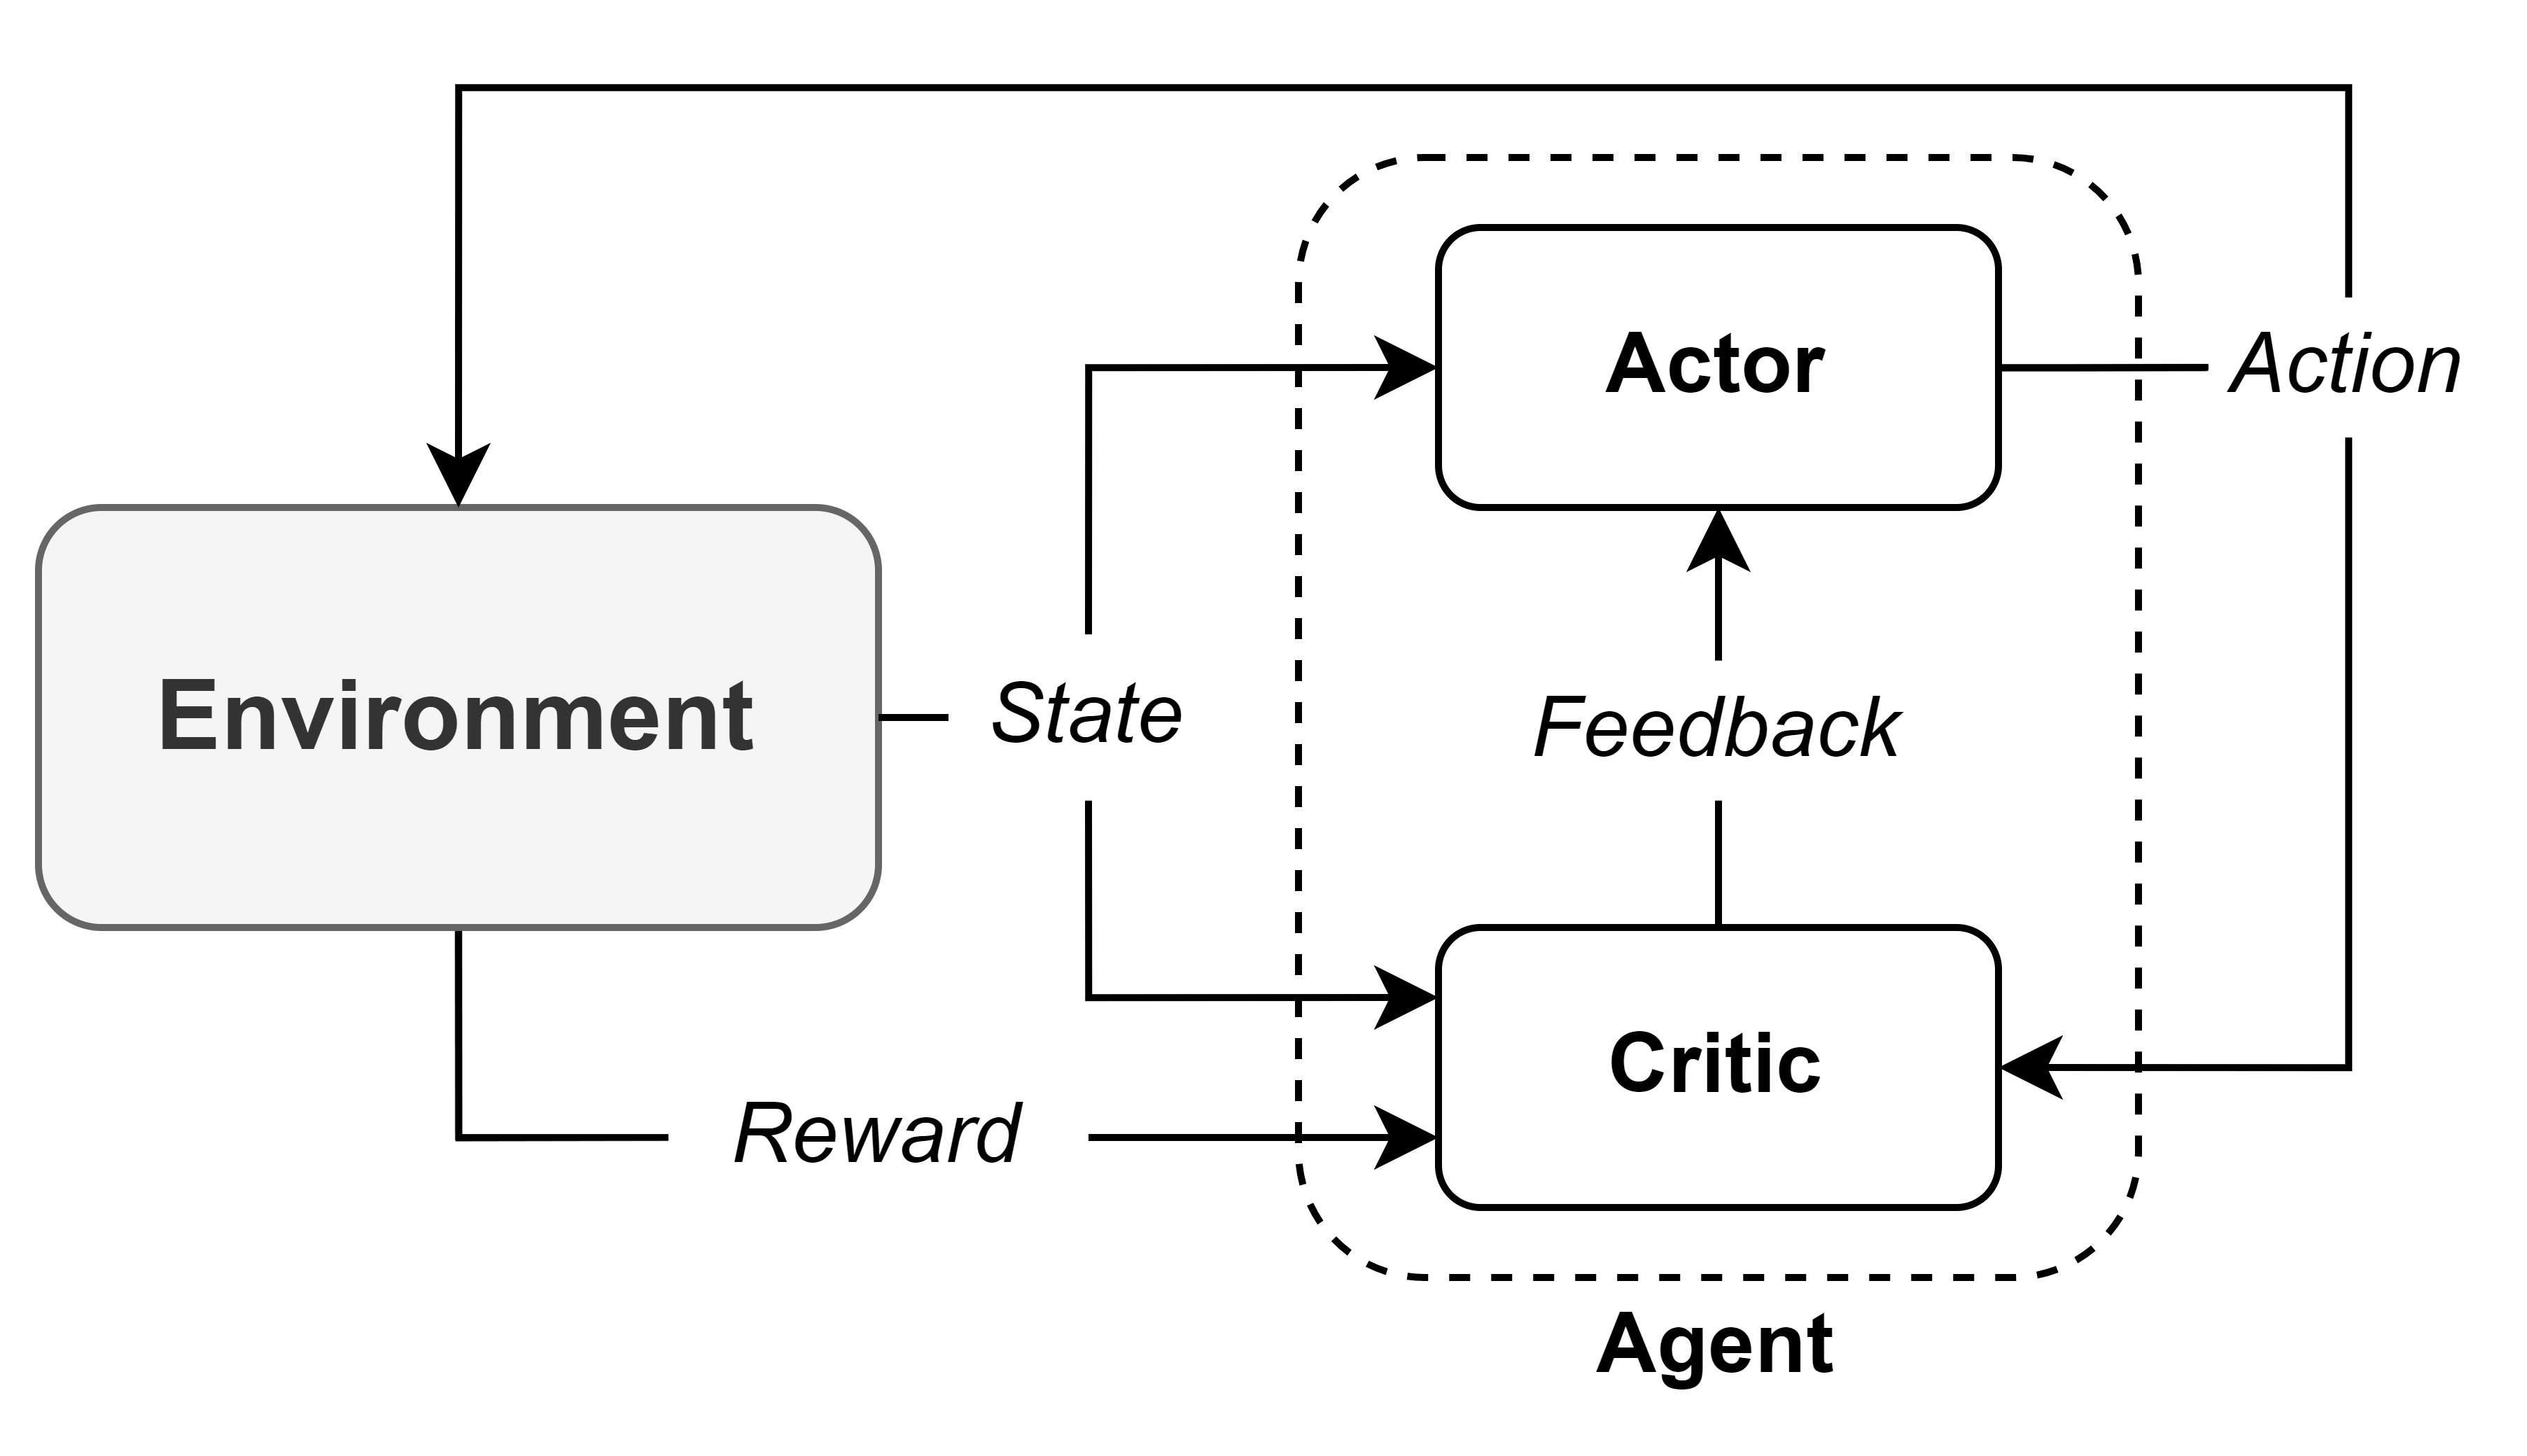
\includegraphics[width=0.6\textwidth]{images/figures/actor-critic.png}
    \caption{The actor-critic framework.}
    \label{fig:actor-critic}
\end{figure}

A common architecture used in DRL is the \textit{actor-critic framework}, shown in Figure \ref{fig:actor-critic}~\cite{barto1983ac,konda1999ac}.
Actor-critic algorithms maintain two complementary components: an actor and a critic.
The actor represents the policy, proposing which action to take in a given state.
The critic estimates a value function that evaluates the quality of the actor's decisions~\cite{barto1983ac,konda1999ac}.
Sometimes the actor and critic make use of a single, shared network, only branching into a separate heads at the very end.
This allows for useful features to be shared by both actor and critic, but risks interference between objectives in more complex environments~\cite{sutton2018rl,konda1999ac}.

Given the observed rewards from the actor's decisions, the critic learns by minimizing the difference between what it expected to happen and what actually occurred, called the \textit{temporal difference} (TD) error~\cite{sutton2018rl,konda1999ac}:
\begin{equation}
    \delta = r_{t+1} + \gamma V(s_{t+1}) - V(s_t)
\end{equation}
Rather than updating the policy solely based on observed returns, the actor is instead guided by the critic through the advantage function~\cite{sutton2018rl}:
\begin{equation}
    A(s, a) = Q(s, a) - V(s)
\end{equation}
The advantage function measures how much better or worse an action performs relative to the average action in the same state.
Positive advantages encourage the policy to increase the probability of selecting an action, while negative advantages discourage it~\cite{sutton2018rl}.
Calculating the true theoretical advantage requires comparing the value of an action against the average of all possible actions, which is often computationally intractable.
Instead, the actor can also learn from the TD error as a sample-based advantage estimate~\cite{sutton2018rl,konda1999ac}.

Proximal policy optimization (PPO) is one of the most widely used DRL algorithms, mostly thanks to its robustness and strong empirical performance~\cite{wang2024drl,schulman2017ppo}.
A key challenge in DRL methods that use gradients to directly update the policy is that large parameter updates may produce a drastically different policy, leading to unstable training or severe performance degradation~\cite{schulman2017ppo}.
PPO addresses this issue by constraining how much the policy is allowed to change during each optimization step.
PPO maximizes the clipped surrogate objective~\cite{schulman2017ppo}:
\begin{equation}
    L^{CLIP}(\theta) = \mathbb{E}\left[ \min\left(r_t(\theta)A_t, \mathrm{clip}\left(r_t(\theta), 1-\epsilon, 1+\epsilon\right)A_t\right) \right],\text{ where } r_t(\theta) = \frac{\pi_\theta(a_t|s_t)}{\pi_{\theta_{\mathrm{old}}}(a_t|s_t)}
\end{equation}
The clipping operation limits the incentive for excessively large policy updates, preventing the optimization from moving too far away from the previous policy while still allowing steady improvement.
PPO is implemented using an actor-critic framework that learns from data collected using the current policy (on-policy learning), and with a special entropy coefficient in its loss function to balance exploration and exploitation~\cite{schulman2017ppo}.
Because of its balance between computational efficiency and stable learning dynamics, PPO has become one of the standard algorithms for deep reinforcement learning~\cite{wang2024drl}.

\subsection{Multi-Agent Reinforcement Learning} \label{sec:rl:marl}
Reinforcement learning agents often have to compete or cooperate with other agents in complex, dynamic multi-agent systems.
Multi-agent reinforcement learning (MARL) is a subfield of reinforcement learning that focuses on the behavior of multiple learning agents that coexist in a shared environment, whether cooperating or competing~\cite{stefano2024marl,zhang2025selfplay}.

In an environment where agents are competing against each other, each agent has its own policy, value function, and reward function.
In this scenario, agents are trying to learn a best response policy: A policy that chooses the optimal action given the policies of other agents.
If all agents are following a best response policy, then the agents are in a \textit{Nash equilibrium}: No agent can improve by (individually) changing its policy~\cite{stefano2024marl,zhang2025selfplay}.
Most environments where two agents compete against each other are modeled as two-player \textit{zero-sum} games, meaning $r_1 = -r_2$.
The Minimax theorem states that any finite two-player zero-sum game has a Nash equilibrium~\cite{neumann1928minimax}.

Both the state and action space in MARL grow exponentially with the number of agents.
Additionally, if the actions are jointly determined by all agents, a single agent's action does not influence the environment in a fixed manner like in single-agent RL.
This means that the best response policy for agents is a moving target and the Markov assumption for MDPs is violated, making training MARL agents a challenging task~\cite{stefano2024marl,zhang2025selfplay}.

One of the most popular frameworks for training an agent in a competitive zero-sum game is \textit{self-play}. In self-play, an agent trains against a past or current version of its own policy, learning solely from the win/loss feedback signal~\cite{stefano2024marl,zhang2025selfplay}.
Although this violates the stationarity assumption underlying classical reinforcement learning, self-play often produces highly capable policies through an automatic curriculum (the experiences get increasingly difficult as the policy improves)~\cite{silver2017alphazero,zhang2025selfplay}.

Other frameworks for training agents in competitive zero-sum games include \textit{fictitious self-play} (the agent plays against the average of its past policies~\cite{heinrich2015fictitioussp}) and \textit{double oracle} (maintain an iteratively expanded subset of active policies for both agents~\cite{bosansky2014doubleoracle}), though regular self-play has already achieved landmark successes in games with large strategic search spaces, including chess, Go, StarCraft II, and Dota 2~\cite{silver2017alphazero,vinyals2019starcraft,berner2019dota}.
These successes demonstrate that high-level strategies can emerge without explicit human guidance when sufficiently powerful reinforcement learning algorithms are combined with large-scale self-play~\cite{silver2017alphazero}.

\section{Continual Learning} \label{sec:cl}
Traditional machine learning is largely built on the assumption that training data is drawn from the same stationary distribution as the data seen after training: Most models are trained once on a fixed dataset and subsequently deployed without further adaptation~\cite{khetarpal2022crl,wang2024cl}.
However, true autonomous agents will continuously encounter new situations, changing environments, and evolving tasks throughout their lifetime, violating this crucial assumption.
In these non-stationary settings, models must be capable of processing new information while preserving previously learned knowledge. 
This learning paradigm is typically referred to as lifelong learning, incremental learning, or \textit{continual learning} (CL)~\cite{wang2024cl}.

Continual learning aims to enable models to learn from a sequence of experiences rather than from a single static dataset~\cite{khetarpal2022crl,wang2024cl}.
As new data becomes available, the model incrementally updates its parameters instead of being retrained from scratch.
Ideally, continual learning allows an agent to continuously improve its performance while not degrading on previously learned tasks.
Achieving this objective is challenging because updating the model to incorporate new information can interfere with knowledge acquired earlier~\cite{wang2024cl,mccloskey1989catastforget}.

A fundamental challenge in continual learning is the \textit{stability-plasticity dilemma}~\cite{wang2024cl}.
Stability refers to the preservation of previously acquired knowledge, while plasticity refers to the ability of a model to incorporate new information and adapt to changes in the environment.
High plasticity allows an agent to learn efficiently when novel tasks or data distributions are encountered, while a highly stable model resists changes that would degrade performance on earlier tasks.
These objectives are inherently conflicting.
Increasing plasticity generally makes the model more susceptible to overwriting existing knowledge, whereas emphasizing stability can prevent the model from learning new information effectively~\cite{wang2024cl,dohare2024plasticity}.
Finding the ideal balance between stability and plasticity is one of the main challenges that continual learning algorithms try to solve~\cite{wang2024cl}.

One of the most prominent issues arising from the stability-plasticity dilemma is \textit{catastrophic forgetting}~\cite{wang2024cl,mccloskey1989catastforget}.
Catastrophic forgetting occurs when learning new information substantially degrades performance on previously learned tasks.
In artificial neural networks, this phenomenon arises because gradient-based optimization updates shared parameters to minimize the loss on the current data, potentially overwriting parameter configurations that were important for previously learned tasks~\cite{mccloskey1989catastforget}.
Since earlier training data is typically unavailable during continual learning, performance on earlier tasks can deteriorate rapidly after training on new ones.
The severity of catastrophic forgetting depends on several factors, including the similarity between tasks, the degree of parameter sharing, the model architecture, and the learning algorithm~\cite{khetarpal2022crl,wang2024cl}.
Tasks that require substantially different representations often induce greater interference than closely related tasks~\cite{wang2024cl}.

Continual learning problems can be categorized according to the information available during training and evaluation. Commonly studied scenarios include~\cite{wang2024cl}:
\begin{itemize}
    \item \textit{Task-incremental learning}: The current task is known during both training and inference.
    The objective is to learn multiple tasks sequentially while maintaining performance on all previously encountered tasks.
    \item \textit{Domain-incremental learning}: The task remains conceptually the same, but the input distribution changes over time.
    The model must adapt to these distribution shifts without relying on explicit task identifiers.
    \item \textit{Class-incremental learning}: New classes become available over time.
    The model must continuously expand its classification capability without forgetting previously learned classes.
\end{itemize}
Formally, a sequence of tasks $\mathcal{T}$ is defined as a series of problem spaces $\{ T_1, T_2, ... , T_N \}$, each defined by a respective dataset $T_t = (\mathcal{X}^t, \mathcal{Y}^t)$, where $\mathcal{X}^t$ is the input feature space and $\mathcal{Y}^t$ is the corresponding output space~\cite{khetarpal2022crl,wang2024cl}.

\subsection{Continual Reinforcement Learning} \label{sec:cl:crl}
Continual reinforcement learning (CRL) is the joint paradigm of continual learning and reinforcement learning.
Reinforcement learning provides an agent-environment framework suitable for studying learning in a continual fashion, making it a natural fit for continual learning~\cite{khetarpal2022crl}.

In CRL, a sequence of tasks $\mathcal{T}$ is defined as a series of distinct MDPs $\{ \mathcal{M}_1, \mathcal{M}_2, ... , \mathcal{M}_N \}$, making the core RL problem non-stationary~\cite{puterman1990mdp}.
Non-stationarity presents several challenges for RL.
Policies that perform well under one environment configuration may become suboptimal after changes occur, while neural networks trained on previous experiences are susceptible to catastrophic forgetting when adapting to new conditions~\cite{khetarpal2022crl,wang2024cl}.
Furthermore, experiences collected under outdated dynamics may become misleading, reducing the effectiveness of replay buffers and value estimation~\cite{khetarpal2022crl}.
Continual reinforcement learning aims to address these challenges and enable agents to learn continuously from evolving environments while retaining previously acquired knowledge.
Depending on the application, the objective may be to maintain performance across a sequence of changing tasks, rapidly adapt to new dynamics, or achieve a balance between the two~\cite{khetarpal2022crl}.

\textit{Regularization-based methods} attempt to identify parameters that are important for previously learned tasks and penalize changes to these parameters during subsequent training.
The objective is to preserve critical knowledge while allowing less important parameters to adapt~\cite{khetarpal2022crl,wang2024cl}.
Prominent methods in this family include Elastic Weight Consolidation (EWC)~\cite{kirkpatrick2017ewc}, Elastic Variational Continual Learning (EVCL)~\cite{batra2024evcl}, and Synaptic Intelligence (SI)~\cite{zenke2017si}.
This family also includes transfer learning methods like Actor-Mimic~\cite{parisotto2015actormimic} and Distral~\cite{teh2017distral}.
These are policy distillation methods that focus on transferring knowledge from a (typically larger) teacher model to a fresh student model~\cite{khetarpal2022crl,zhu2023tl}.

\textit{Replay-based methods} store or generate examples from previously encountered tasks and interleave them with new experiences during training.
By periodically revisiting earlier data, the model reinforces previously learned knowledge~\cite{khetarpal2022crl,wang2024cl}.
This comes at the cost of learning off-policy, which is seen as a weaker alternative to on-policy learning in the context of continual learning.
Old experiences can become outdated and start reinforcing bad habits, possibly corrupting the model and preventing it from converging to an optimal policy~\cite{wang2024cl,hasselt2018deadlytriad}.
Prominent methods that try to mitigate this include Continual Learning with Experience And Replay (CLEAR)~\cite{rolnick2019clear} and Efficient Diversity-based Experience Replay (EDER)~\cite{zhao2024eder}.

\textit{Parameter-isolation methods} allocate separate subsets of model parameters to different tasks.
Rather than modifying parameters that encode existing knowledge, these methods expand or partition the network to accommodate new information~\cite{khetarpal2022crl,wang2024cl,zhu2023tl}.
A prominent method in this family is Progressive Neural Networks (PNNs), which append the network with horizontal layers (\textit{columns}) for each task, with lateral connections to previous layers to reuse previously learned representations~\cite{zhu2023tl,rusu2016pnn}.
A similar method is PathNet, which dynamically allocates sections of a fixed-size network to separate tasks~\cite{zhu2023tl,fernando2017pathnet}.
For transformer-based models there is the well-established Low-Rank Adaptation (LoRA), typically used for large language models~\cite{hu2022lora}.
This family also includes specialized optimization methods like ReDo~\cite{sokar2023redo} and Continual Backprop~\cite{dohare2021cbp}, which selectively reinitialize stagnant neurons to combat loss of plasticity, though recent work has shown that these methods only have a limited benefit over fine-tuned learning with L2 regularization in continual reinforcement learning settings~\cite{dohare2024plasticity,lyle2023plasticity}.

\section{Competitive Pokémon (VGC)} \label{sec:vgc}
Pokémon is the highest-grossing media franchise in the world, with an estimated total revenue exceeding \$100 billion and a global player base numbering in the millions~\cite{angliss2025vgc}.
In 2008, the Pokémon Company launched the franchise's first official video game tournaments under the name Pokémon Video Game Championship (VGC).
VGC is still the name of the official Esports circuit of the Pokémon franchise, with frequent tournaments being hosted around the world where players compete for significant cash prizes and international prestige~\cite{angliss2025vgc,vgc-rules-regulations}.
At the most abstract level, VGC consists of two tightly-coupled phases: \textit{team building} and \textit{battling}.
While game updates could have a significant impact on both phases, the scope of this thesis will focus solely on the domain of battling.

\subsection{Rules and Mechanics} \label{sec:vgc:mechanics}
A VGC match (hereafter referred to as \textit{battle}) consists of two players, each using a preassembled team of six distinct Pokémon.
A Pokémon is uniquely identified through an HP, attack, special attack, defense, special defense, and speed stat, one or two types, up to three possible abilities, and a set of possible moves.
In the team building phase, players can customize their Pokémon by slightly changing the Pokémon's stats, choosing their ability and up to four of its moves, and giving them a unique held item.
None of this vast amount of customization is initially visible to the opponent, leading to a complex partial observability that acts as one of the key challenges of VGC, both for human players and for the development of competitive agents.
\textcite{angliss2025vgc} estimate the size of the configuration space in VGC to be around $10^{139}$, far exceeding common strategic benchmark games such as Dota or StarCraft.

To account for this vast partial observability, VGC has recently adapted an open team sheets (OTS) format, meaning players can observe various aspects of each other's teams such as moves, items, and abilities~\cite{vgc-rules-regulations}.
While this does bring the size of the information set (the set of all possible states given a partial observation of the game) down significantly, keeping the underlying stat distributions concealed still gives a lower-bound of $10^{58}$ possibilities~\cite{angliss2025vgc}.

VGC is set in the double battles format, meaning each player has up to two Pokémon active on the field at once.
Each battle begins with a team preview phase, during which each player selects four of their six Pokémon to bring into battle.
The first two selected will be active at the start of the battle, while the other two selected will be available to switch in later.

Once the battle begins, both players select the respective moves of their Pokémon.
While VGC is mainly a turn-based game, moves for each turn are selected simultaneously by both players.
Typical moves include attacking one or both of the opponent's Pokémon, switching your own Pokémon to one not currently on the field, or opting for a utility-based move.

Move outcomes typically involve a large amount of random chance.
Most moves have a chance to miss their target, activate a secondary effect, or both at once.
Pokémon can also be inflicted with status conditions like paralysis, freeze, or sleep, all of which come with the chance of being unable to move for a turn.
Additionally, all attacking moves have a 1/16 chance to be a critical hit, dealing $1.5\times$ damage and ignoring all defensive modifiers.

The objective of a battle is to knock out all of the opponent's Pokémon before your own team is eliminated.
Formally speaking, a battle can be modeled as a two-player zero-sum partially observable stochastic game:
\begin{equation}
    \mathcal{G}(c_1, c_2) = \left\langle \mathcal{S}, \left\{\mathcal{O}_i\right\}, \left\{\mathcal{A}_i\right\}, \mathcal{P}, \mathcal{R}, c_1, c_2 \right\rangle
\end{equation}
Where $\mathcal{S}$ is the full battle state, $\mathcal{O}_i \subseteq \mathcal{S}$ is player $i$'s observation, $\mathcal{A}_i$ is player $i$'s action set, $\mathcal{P}(s^\prime | s, a_1, a_2)$ is the stochastic transition function, $\mathcal{R}(s) \in \{-1, 1\}$ is the terminal reward for player 1 in state $s$, and $c_i$ is the team configuration of player $i$~\cite{angliss2025vgc}.

\subsection{Regulations} \label{sec:vgc:regulations}
While VGC can be played with any selection of Pokémon, official tournaments and other competitions tend to restrict the legality of some, typically more powerful, Pokémon to create more varied metagames.
The Pokémon Company defines specific rulesets, called \textit{regulations}, that determine which Pokémon are legal to use in official tournaments, typically lasting for two to three months at a time~\cite{vgc-rules-regulations}.
We refer to the formal sets containing all Pokémon that are legal to use as \textit{regulation sets}.
When a new VGC game releases, regulation sets typically start off small and only grow larger over time, with each new regulation set typically being a strict superset of the previous regulation sets.
It is uncommon for old regulations to be played once they are no longer active, unless they become the active ruleset again.

In this thesis we will focus on the latest VGC games for which full regulation-data is available, those being the \textit{Pokémon Scarlet} \& \textit{Pokémon Violet} games which ran the official VGC circuit from 2022 to 2026~\cite{vgc-rules-regulations}.
These games saw a total of 10 different regulations during this span, an overview of which can be found in Table \ref{tab:regulations}.

\begin{table}[ht]
\centering
    \begin{tabular}{ccl}
    \textit{Regulation} & \textit{\#Legal Pokémon} & \multicolumn{1}{c}{\textit{Description}} \\ \hline
    \textbf{A} & 380 & Base Pokédex \\
    \textbf{B} & 394 & Allows Paradox Pokémon \\
    \textbf{C} & 398 & Allows the four Treasures of Ruin \\
    \textbf{D} & 494 & Allows Pokémon from Pokémon HOME \\
    \textbf{E} & 593 & Allows Pokémon from the Kitakami Pokédex \\
    \textbf{F} & 698 & Allows Pokémon from the Blueberry Pokédex \\
    \textbf{G} & 718 & Allows Restricted Pokémon (max. 1 per team) \\
    \textbf{H} & 631 & Bans Paradox and Legendary Pokémon \\
    \textbf{I} & 718 & Allows Restricted Pokémon (max. 2 per team) \\
    \textbf{J} & 733 & Allows Mythical Pokémon (max. 2 per team) \\ \hline
    \end{tabular}
    \caption{All VGC regulations in the \textit{Pokémon Scarlet} \& \textit{Pokémon Violet} games~\cite{vgc-rules-regulations}. Legal Pokémon numbers are estimates and may vary due to ambiguous sources.}
    \label{tab:regulations}
\end{table}
\vspace{-\baselineskip} % make gap smaller
\begin{align} \label{eq:regulations}
    \textbf{A} \subset \textbf{B} \subset \textbf{C} \subset \textbf{D} \subset \textbf{E} \subset \textbf{F} \subset \textbf{G} = \textbf{I} \subset \textbf{J} && \textbf{A} \subset \textbf{H} \subset \textbf{F} \subset \textbf{G} = \textbf{I} \subset \textbf{J}
\end{align}

Relations between different regulation sets are given by Equation \ref{eq:regulations}.
We can observe that almost all regulation sets are supersets of the regulation sets that came before, regulation \textbf{H} being the only exception (regulations \textbf{G} and \textbf{I} have identical regulation sets, but differ in the way teams can be composed).
Each regulation has its own unique metagame that vastly differs from the other regulations, even if the difference on paper may seem minimal.
For example, observe in Table \ref{tab:regulations} that regulation \textbf{C} only has four more legal Pokémon than regulation \textbf{B}.
While this makes the set difference between their regulation sets quite small, these four additional Pokémon that are legal in regulation \textbf{C} are some of the most powerful in the game.
This results in the vast majority of teams in regulation \textbf{C} featuring at least one of these four meta-defining Pokémon, making playing regulation \textbf{C} vastly different to regulation \textbf{B}, even though the difference between the two may seem minimal at a glance.

\subsection{VGC-Bench} \label{sec:vgc:vgc-bench}
The main work of this thesis is based on and built on top of \textit{VGC-Bench}, a comprehensive benchmark that provides a multi-agent reinforcement learning environment for VGC, various baseline agents, meta-relevant teams for each regulation, and a dataset of trajectories from human players~\cite{angliss2025vgc}.

An observation of a state is given by VGC-Bench as a concatenation of features of all 12 Pokémon in the battle, shaped as $12 \times (g + s + p)$ where $g$ is a vector of global features (e.g. weather), $s$ is a vector of the Pokémon's side's features (e.g. tailwind), and $p$ is a vector of the Pokémon's specific features (e.g. HP).
The action space is a masked joint action space between the four active Pokémon, with each Pokémon having a worst case of 107 possible actions per turn~\cite{angliss2025vgc}.

VGC-Bench implements 11 baseline agents: three basic heuristic agents, an LLM agent, a behavior cloning agent (trained to match the decision-making of human players on a large set of trajectories collected from all regulations), a self-play RL agent, a fictitious self-play RL agent, a double oracle RL agent, and three fine-tuned versions of the behavior cloning agent using the three mentioned RL techniques respectively.
All RL agents share the same underlying architecture (shown in Figure \ref{fig:vgcbench-architecture}) and are trained using PPO on the same selection of teams~\cite{angliss2025vgc}.
Evaluation is done using 1000 episodes of cross-play between different agents, either using the same set of teams seen during training (the \textit{in-distribution} set) or with a completely new set of teams (the \textit{out-of-distribution} set).
The exact hyperparameters of the training process can be found in Table \ref{tab:hyperparam-vgcbench}.

\begin{table}[ht]
    \centering
    \begin{tabular}{lr}
    \textbf{Parameter} & \textbf{Value} \\ \hline
    \textbf{Learning Rate} & $\text{1e-5} \times 0.1^{(1 - p)}$ \\
    \textbf{Discount Factor ($\gamma$)} & 1.0 \\
    \textbf{GAE Lambda ($\lambda$)} & 0.95 \\
    \textbf{Clip Range} & 0.2 \\
    \textbf{Entropy Coefficient} & 0.001 \\
    \textbf{Value Function Coefficient} & 0.5 \\
    \textbf{Max Gradient Norm} & 0.5 \\
    \textbf{Number of Steps per Update} & $24 \times 128$ \\
    \textbf{Batch Size} & 512 \\
    \textbf{Number of Epochs} & 10 \\
    \textbf{Total Timesteps} & $5\,013\,504$ \\ \hline
    \end{tabular}
    \caption{Hyperparameters used for all reinforcement learning experiments in VGC-Bench~\cite{angliss2025vgc}.}
    \label{tab:hyperparam-vgcbench}
\end{table}

\begin{figure}[ht]
    \centering
    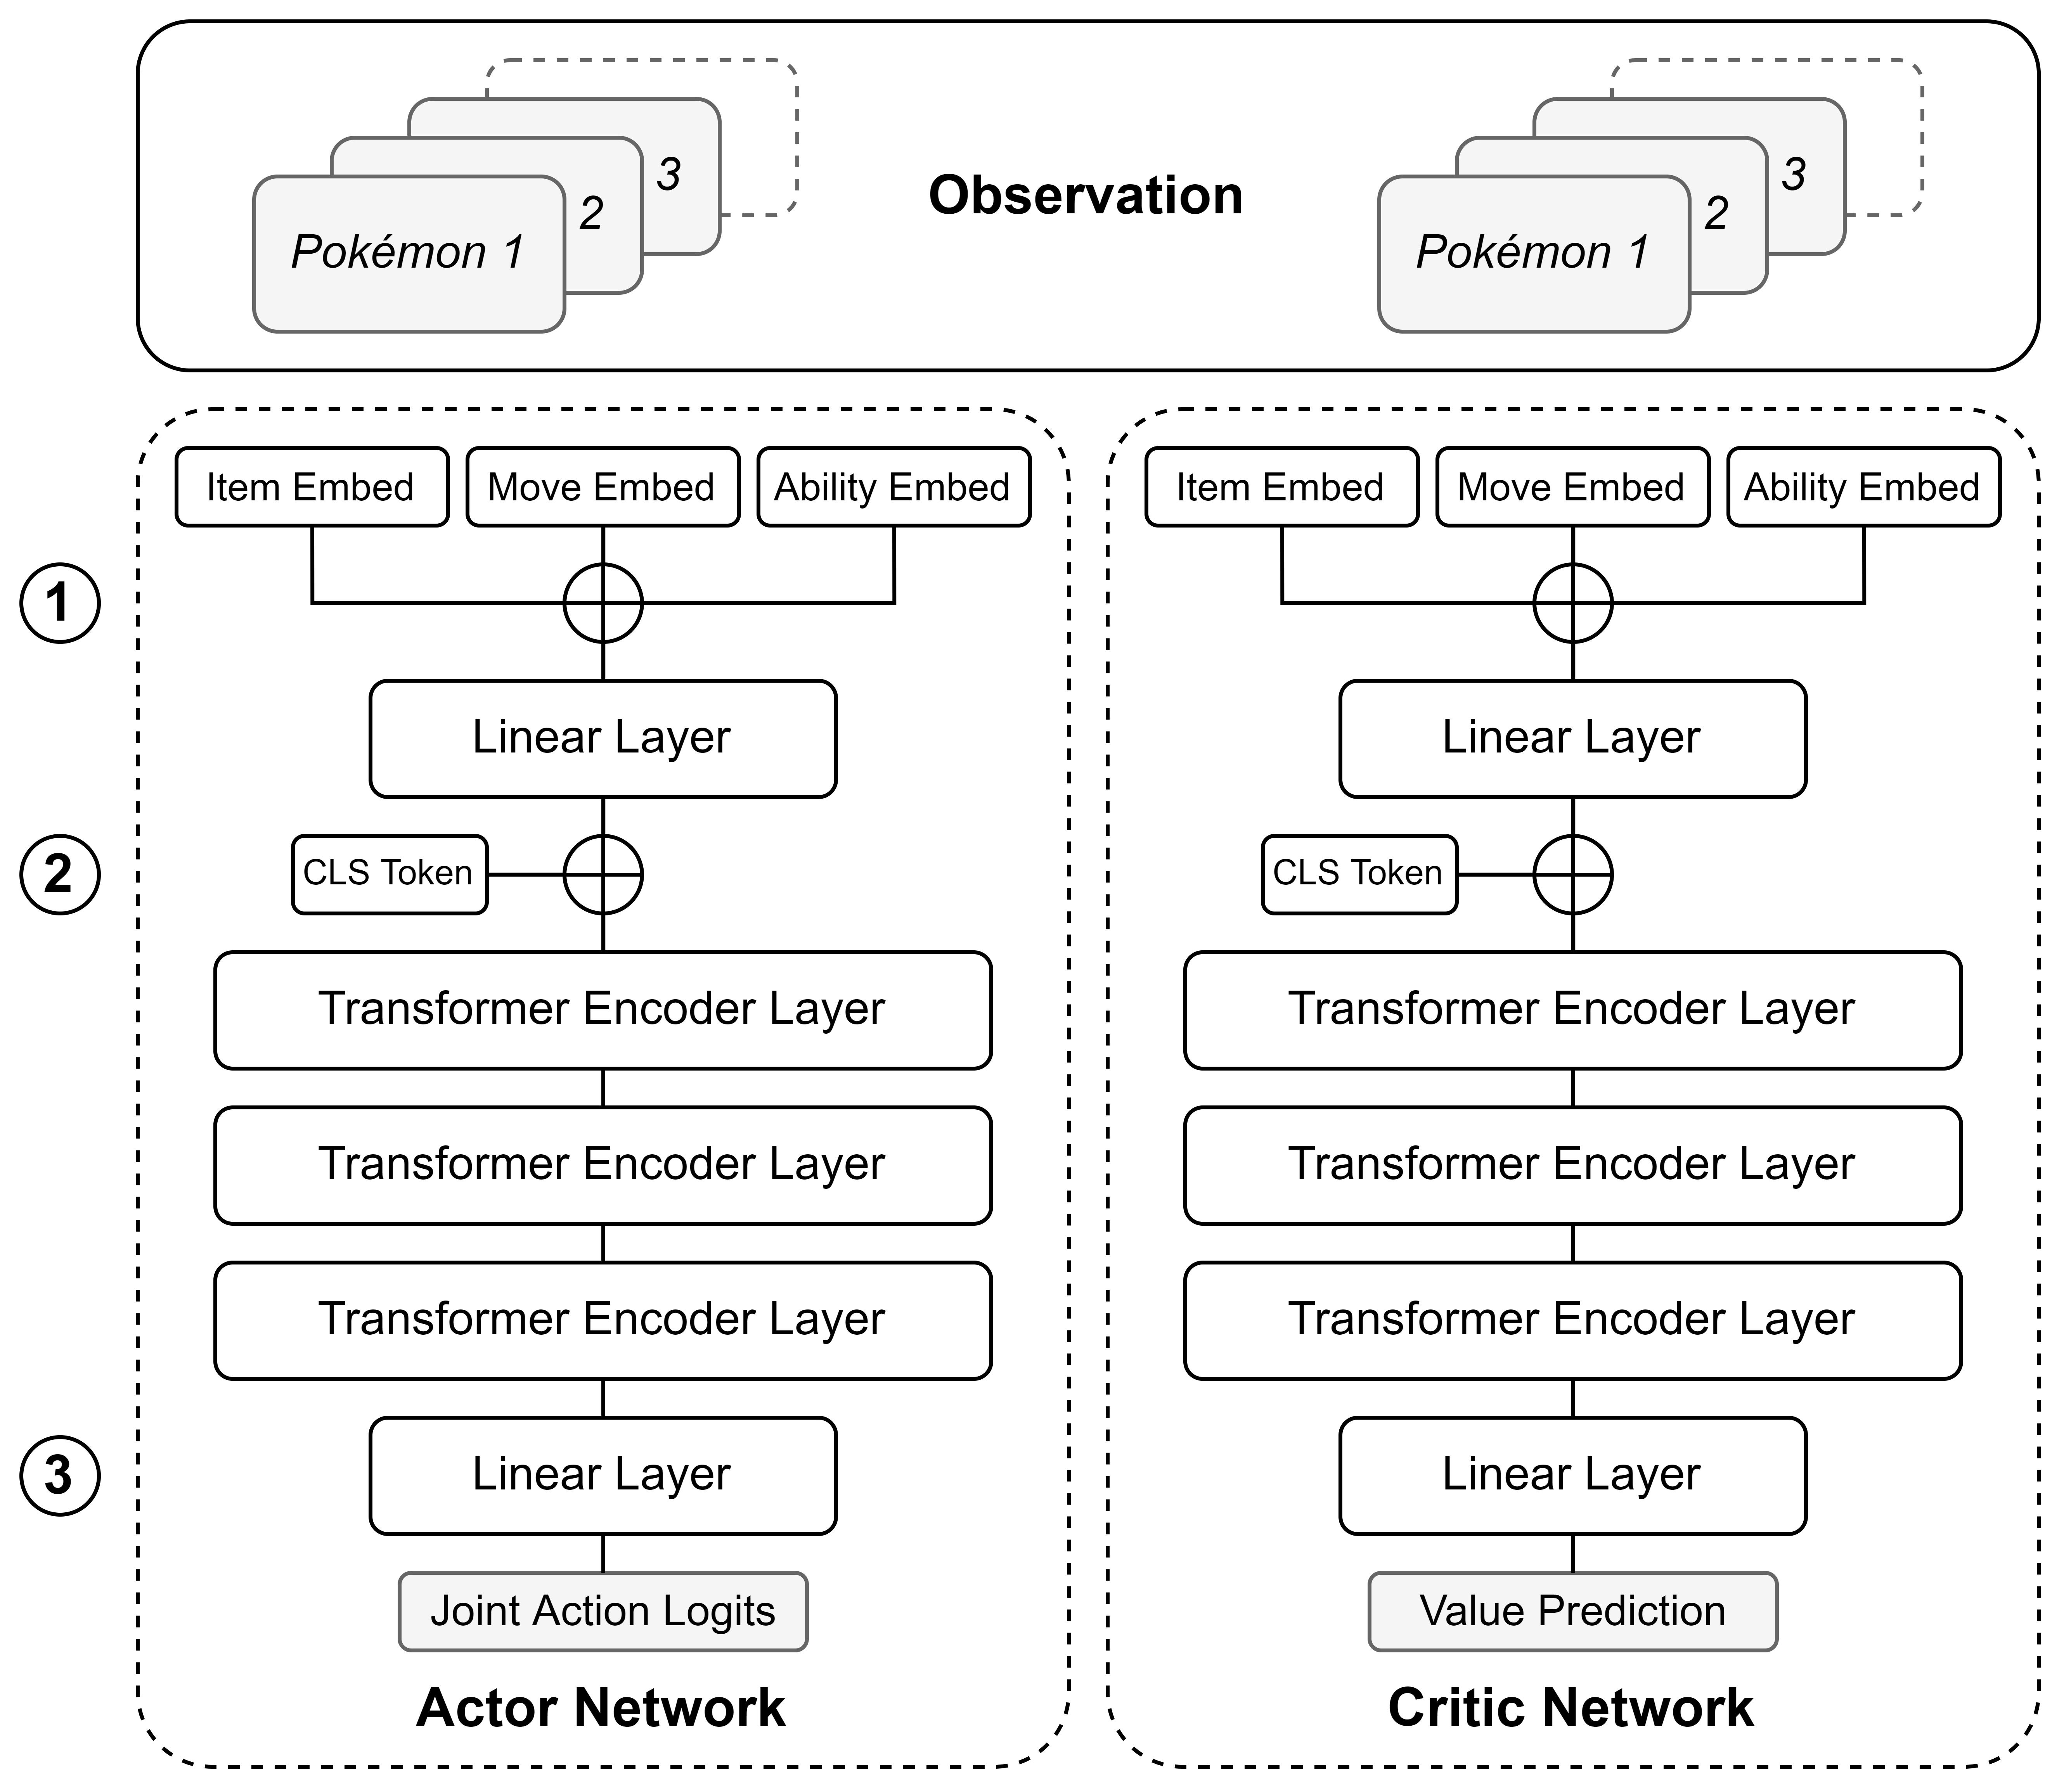
\includegraphics[width=0.95\textwidth]{images/figures/vgc-bench.png}
    \caption{The architecture used by all RL agents in VGC-Bench~\cite{angliss2025vgc}. All agents use an actor-critic framework with the same network architecture, but without direct parameter sharing. A forward pass through the network can be dissected into the following steps: \textbf{(1)} All Pokémon in the observation have their items, moves, and abilities embedded into 32-dimensional latent representations. These representations, together with other numerical features, are concatenated and projected to a single 256-dimensional latent space. \textbf{(2)} The latent vector is concatenated with an aggregation token (typically referred to as the \textit{CLS token}~\cite{devlin2019bert}), before passing through a three-layer, encoder-only transformer model with four attention heads. \textbf{(3)} The output of the transformer is either projected to action logits (actor), or to a value prediction (critic).}
    \label{fig:vgcbench-architecture}
\end{figure}

The findings of VGC-Bench show that behavior cloning fine-tuned with RL techniques can consistently beat other agents, and is even able to beat professional VGC players under the right circumstances.
They furthermore show that RL agents perform best when the amount of teams they see during training is kept to a minimum, though agents who see more teams during training are able to generalize better to unseen teams~\cite{angliss2025vgc}.

\newpage
%
% Analysis
%
\chapter{Preliminary Experiments} \label{sec:preliminary}
In this chapter we perform preliminary experiments to investigate the effects of non-stationarity and the transferability of RL agents in VGC.
The goal of these experiments is to answer the following questions:

\begin{enumerate}
    \item What effect does non-stationarity have on the performance and generalization of reinforcement learning agents in VGC?
    \item To what extent are reinforcement learning agents able to maintain performance under non-stationarity without any continual learning techniques?
\end{enumerate}

We first formalize our problem statement outlined in Chapter \ref{sec:introduction}:
Let $A_t$ be an agent that is trained from scratch on a unique version $t$ of a two-player zero-sum game $\mathcal{G}_t$ for $n$ steps.
Our goal is to identify or propose training paradigms that allow $A_t$ to outperform (i.e. have a higher win rate than) agent $A_{t+1}$ on $\mathcal{G}_{t+1}$, in at most $n$ additional training steps.
Additionally, we make the following assumptions:

\begin{assumption} \label{ass:increasing}
    $t$ is monotonically increasing.
\end{assumption}

\begin{assumption} \label{ass:task}
    $\mathcal{G}_{t+1}$ has the same action space and reward function as $\mathcal{G}_{t}$.
\end{assumption}

\begin{assumption} \label{ass:availability}
    Knowledge about $\mathcal{G}_{t+1}$ is unavailable when training on $\mathcal{G}_{t}$.
\end{assumption}

For VGC, this amounts to agent $A_0$ being trained on regulation \textbf{A}, after which it will have to transfer its learned knowledge to regulation \textbf{B}, then to regulation \textbf{C}, etc.
Under assumption \ref{ass:increasing}, no regulation will be revisited after it is played.
Under assumption \ref{ass:task}, we can classify this problem as a \textit{domain-incremental learning} problem, where agents have to adapt to a non-stationary input distribution (different teams in different regulations).

As discussed in Chapter \ref{sec:vgc:vgc-bench}, VGC-Bench provides six different RL agents that could serve as the basis for experiments in this thesis.
Although the fine-tuned behavior cloning agents show the best results, the behavior cloning model is trained on trajectories of all regulations~\cite{angliss2025vgc}.
Consequently, choosing any of the three fine-tuned behavior cloning agents would violate assumption \ref{ass:availability}.
Out of the remaining three RL agents, we opt for the \textit{regular self-play} model, because of its well-established position in the literature.

Another important parameter for training agents using VGC-Bench is the number of teams in an agent's in-distribution set (the number of teams the agent sees during training).
\textcite{angliss2025vgc} consider a variety of numbers of teams seen during training, ranging from just one team up to 64 unique teams per regulation.
Their findings show that, although larger in-distribution sets lead to worse overall performance, they do lead to significantly better generalization to out-of-distribution teams~\cite{angliss2025vgc}.
Additionally, a larger in-distribution set also decreases the variance caused by how this set is sampled from the pool of all available teams.
Since regulations define which teams can be sampled into the in-distribution set, we speculate that agents trained with a larger in-distribution set can generalize better to different regulations than agents trained with a smaller in-distribution set.
For this reason, we train all agents using the largest number of teams considered by \textcite{angliss2025vgc}: 64 unique teams per regulation.

\section{Zero-Shot Transfer} \label{sec:preliminary:transfer}
To establish to what extent non-stationarity harms the performance of RL agents, we investigate whether RL agents trained on different regulations are capable of zero-shot transfer to other regulations.
We train 10 RL agents using regular self-play, one on each of the 10 regulations shown in Table \ref{tab:regulations}, using the same hyperparameters as VGC-Bench (shown in Table \ref{tab:hyperparam-vgcbench}).
We evaluate by running 1000 episodes of cross-play between all agents in every regulation. The results of this experiment can be found in Figure \ref{fig:zeroshot-indist}.

\begin{figure}[ht]
    \centering
    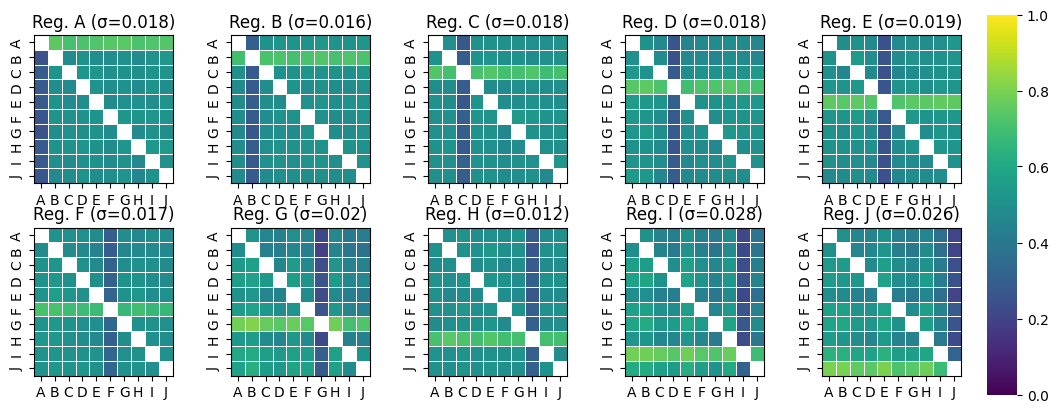
\includegraphics[width=\textwidth]{images/preliminary/zero-shot-in-dist.png}
    \caption{Win rates of the row player over 1000 episodes and three seeds, evaluated in-distribution on each regulation. Letters on the axes represent the regulation the agent is trained on. More in-depth figures for every regulation can be found in Appendix \ref{app:figures}.}
    \label{fig:zeroshot-indist}
\end{figure}

We can observe in Figure \ref{fig:zeroshot-indist} that every agent can consistently win in the regulation that they are trained on, though it should be noted that the teams used for cross-play are all sampled from the in-distribution set of the agent trained on the regulation, potentially biasing the results in favor of that agent.
To evaluate the generalization of the agents to unseen teams, we run a second cross-play experiment using the out-of-distribution set of the agent trained on the regulation, meaning none of the teams have been seen by any agent before.
The results of this experiment can be found in Figure \ref{fig:zeroshot-outofdist} (note that regulations \textbf{B}, \textbf{E}, and \textbf{J} are excluded because there are not enough teams available for a full out-of-distribution set).

\begin{figure}[H]
    \centering
    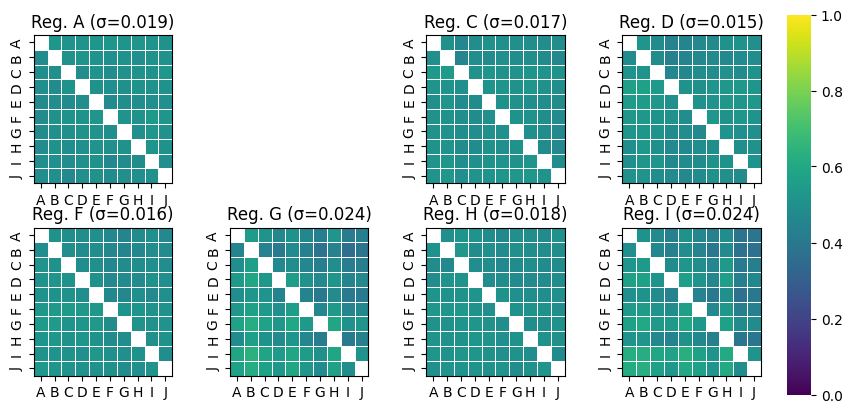
\includegraphics[width=0.85\textwidth]{images/preliminary/zero-shot-out-of-dist.png}
    \caption{Win rates of the row player over 1000 episodes and three seeds, evaluated out-of-distribution on each regulation (excluding regulations \textbf{B}, \textbf{E}, and \textbf{J}). Letters on the axes represent the regulation the agent is trained on. More in-depth figures can be found in Appendix \ref{app:figures}.}
    \label{fig:zeroshot-outofdist}
\end{figure}

We can observe in Figure \ref{fig:zeroshot-outofdist} that the out-of-distribution results are a lot less clear than the in-distribution results shown in Figure \ref{fig:zeroshot-indist}, but, especially in later regulations, there appears to still be an advantage for the agents trained in the same regulation that the cross-play is performed in.

To verify our results, we define our null hypothesis $H_0$ to be that an agent trained on regulation $t$ performs worse than an agent trained on any regulation $\tau \neq t$ when playing in regulation $t$.
We define our significance level to be $\alpha=0.05$.
We can use a Binomial test with $n=1000$ and an expected win rate of $p < 0.5$ to calculate the p-values of the win rates of each row player in the regulation they are trained on.
These p-values are shown in Figure \ref{fig:zeroshot-pvalues}.

\begin{figure}[ht]
    \centering
    \begin{subfigure}{.4\textwidth}
        \centering
        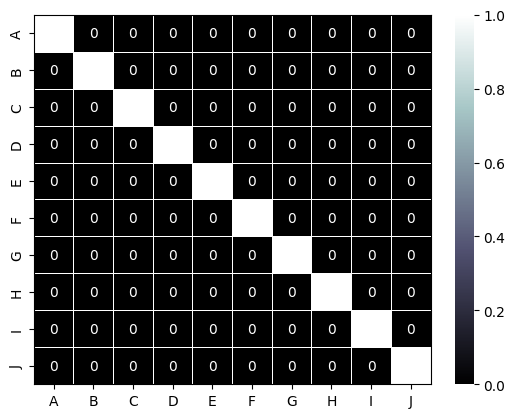
\includegraphics[width=\textwidth]{images/preliminary/zero-shot-in-dist-pvalues.png}
        \caption{In-distribution.}
        \label{fig:zeroshot-pvalues-indist}
    \end{subfigure}
    \hfill
    \begin{subfigure}{.5\textwidth}
        \centering
        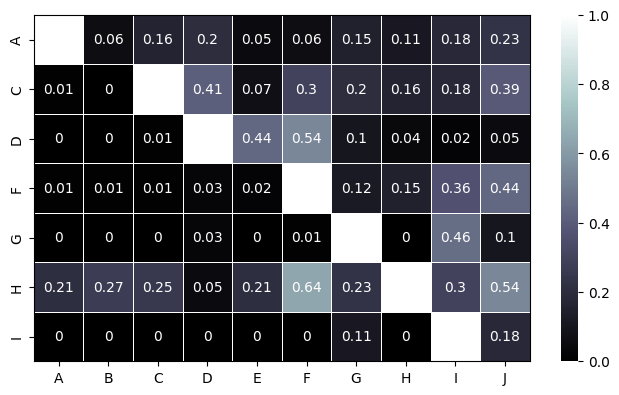
\includegraphics[width=\textwidth]{images/preliminary/zero-shot-out-of-dist-pvalues.png}
        \caption{Out-of-distribution.}
        \label{fig:zeroshot-pvalues-outofdist}
    \end{subfigure}
    \caption{P-values of the win rates of the row player in the regulation that they are trained on. Letters on the axes represent the regulation the agent is trained on.}
    \label{fig:zeroshot-pvalues}
\end{figure}

Observe that all p-values are smaller than 0.05 in Figure \ref{fig:zeroshot-pvalues-indist}, meaning we can reject $H_0$ and conclude that the result for in-distribution cross-play is statistically significant: RL agents are not capable of zero-shot transfer to different regulations.
For Figure \ref{fig:zeroshot-pvalues-outofdist}, things are more complicated.
We can see a general trend emerge that p-values are smaller than 0.05 when agents are evaluated against agents trained on a previous regulation, but larger than 0.05 when evaluated against agents trained on a future regulation, though both of these trends do have exceptions.
We suspect this may be because of the superset relation between different regulations, which would also explain why regulation \textbf{H} seems to be an exception to the general trend.

For the out-of-distribution cross-play results, we can tentatively reject $H_0$ for cases where an agent plays against an agent trained on a previous regulation, and tentatively retain $H_0$ for cases where an agent plays against an agent trained on a future regulation.
This means that, generally speaking, RL agents are capable of zero-shot transfer to future regulations when neither agent has seen the teams before, but incapable of zero-shot transfer in any other scenario.

\section{Full Fine-Tuning} \label{sec:preliminary:finetune}
To establish to what extent RL agents can maintain performance under non-stationarity without using any continual learning techniques, we investigate whether we can transfer the agents trained in Chapter \ref{sec:preliminary:transfer} to other regulations using full fine-tuning.

Staying in line with the problem statement defined at the beginning of this chapter, we start with an agent trained on regulation \textbf{A}.
This agent is then fine-tuned to regulation \textbf{B}, then to regulation \textbf{C}, etc.
Fine-tuning is always done for the same number of steps and using the same hyperparameters as regular training (shown in Table \ref{tab:hyperparam-vgcbench}) to provide an upper bound of the expected performance.
After fine-tuning on a regulation, we evaluate the fine-tuned agent by having it play an agent trained from scratch in that regulation for 1000 episodes.
The results for this experiment can be found in Figure \ref{fig:finetune}.

\begin{figure}[ht]
    \centering
    \begin{subfigure}{.5\textwidth}
        \centering
        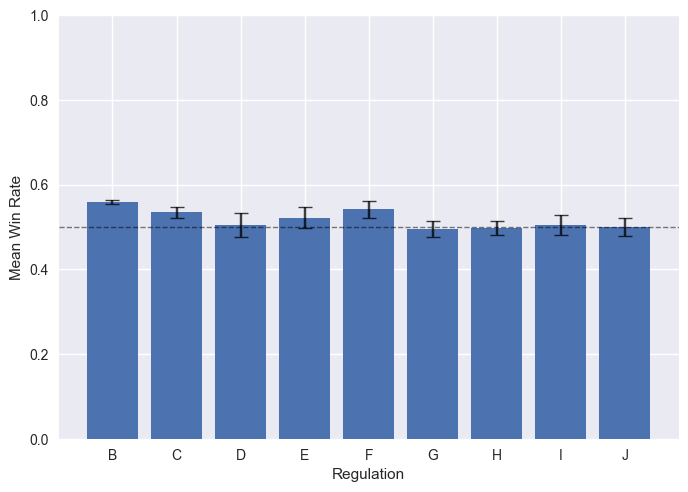
\includegraphics[width=\textwidth]{images/preliminary/finetune-in-dist.png}
        \caption{In-distribution.}
        \label{fig:finetune-indist}
    \end{subfigure}%
    \begin{subfigure}{.5\textwidth}
        \centering
        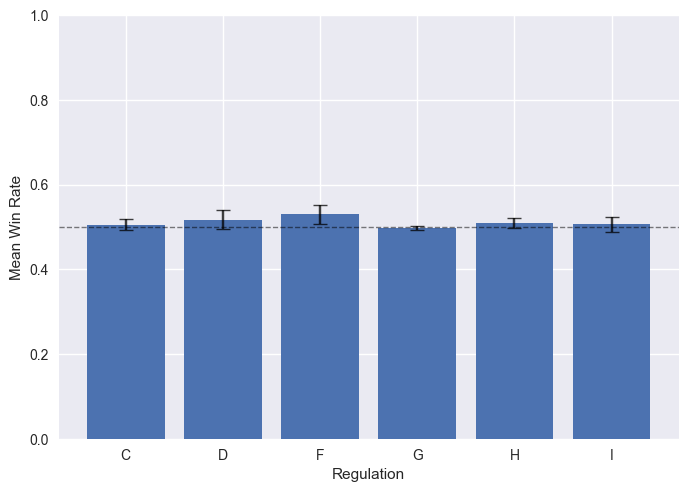
\includegraphics[width=\textwidth]{images/preliminary/finetune-out-of-dist.png}
        \caption{Out-of-distribution.}
        \label{fig:finetune-outofdist}
    \end{subfigure}
    \caption{Mean win rates of fine-tuned agents against agents trained from scratch. Evaluated over 1000 episodes and three seeds on each regulation. More in-depth figures can be found in Appendix \ref{app:figures}.}
    \label{fig:finetune}
\end{figure}

To verify these results, we define our null hypothesis $H_0$ to be that an agent $\phi$ is equally skilled or worse than an agent $\psi$, and we define our significance level to be $\alpha=0.05$.
We can use a Binomial test with $n=1000$ and an expected win rate of $p \leq 0.5$ to calculate the p-values of the win rates of agent $\phi$.
These p-values can be found in Figure \ref{fig:finetune-pvalues}.

\begin{figure}[H]
    \centering
    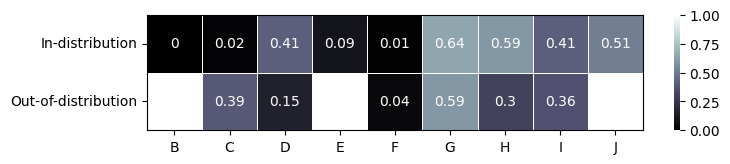
\includegraphics[width=\textwidth]{images/preliminary/finetune-pvalues.png}
    \caption{P-values of the mean win rates of fine-tuned agents against agents trained from scratch. Letters on the horizontal axis represent the regulation the agents are trained or fine-tuned on.}
    \label{fig:finetune-pvalues}
\end{figure}

The results shown in Figures \ref{fig:finetune} and \ref{fig:finetune-pvalues} are quite mixed.
While there are cases where we see an agent experience positive transfer and beat an agent trained from scratch (particularly in the earlier regulations and when evaluating using in-distribution teams), $H_0$ is retained for the majority of cases.
This leads us to tentatively conclude that, in the best case, positive transfer without continual learning is possible short-term, but becomes harder as the non-stationarity increases over time.

\section{Further Analysis} \label{sec:preliminary:analysis}
One trend visible in Figure \ref{fig:finetune} is that the positive transfer is clearly visible in regulation \textbf{F}, but starts to collapse in regulation \textbf{G}, both in-distribution and out-of-distribution.
We decide to analyze these two cases more closely, as any insights gained here could potentially help us prolong the positive transfer using continual learning.

To gather more data about these two cases, we run 100 additional episodes of cross-play on regulations \textbf{F} and \textbf{G}, both in-distribution and out-of-distribution, collecting statistics such as action probabilities, action logits, and value predictions for every observation from three agents: The agent trained on the regulation from scratch, the agent fine-tuned up to the regulation, and the agent fine-tuned up to the previous regulation (the source agent of the other fine-tuned agent).

Our first experiment focuses on the similarity between the action probabilities, which should show us how similar the agents are in their decision making when given the same observation.
We use the Jensen-Shannon (JS) distance, a symmetric version of the Kullback-Leibler (KL) divergence that is bounded to $[0,1]$ (lower values indicating more similar probability distributions), to calculate the distance between two action probability distributions~\cite{dagan1997jsdistance}.
These results, plotted against the normalized depth of the observation (how many turns into the battle it was recorded), can be found in Figure \ref{fig:jsd}.

\begin{figure}[H]
    \centering
    \begin{subfigure}{.5\textwidth}
        \centering
        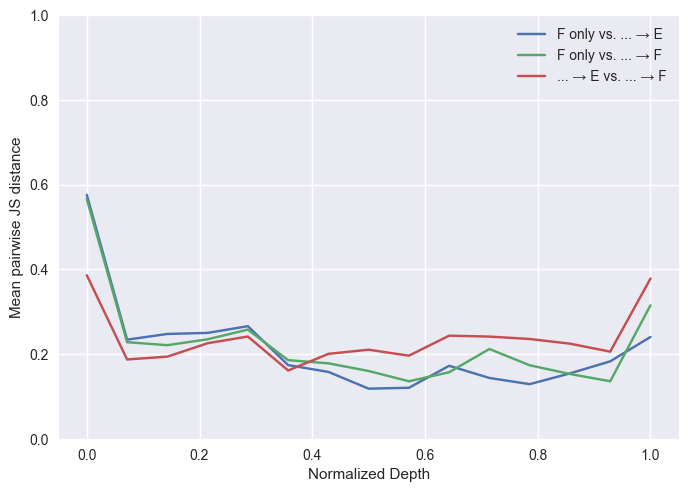
\includegraphics[width=\textwidth]{images/preliminary/jsd-depth-regf-indist.png}
        \caption{Regulation \textbf{F}, in-distribution ($n=974$).}
        \label{fig:jsd-regf-indist}
    \end{subfigure}%
    \begin{subfigure}{.5\textwidth}
        \centering
        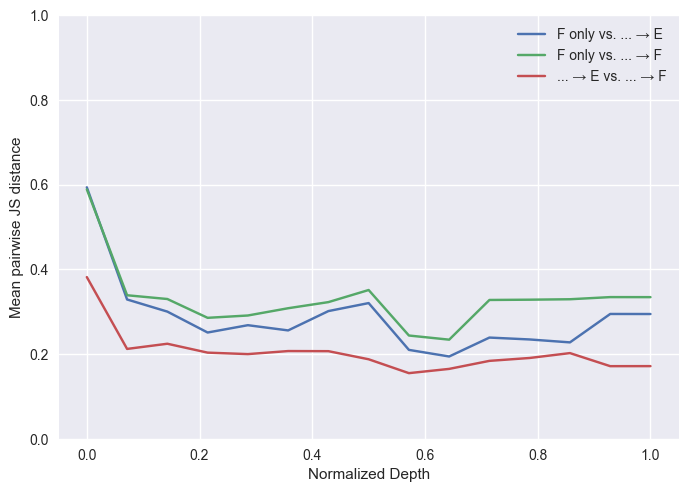
\includegraphics[width=\textwidth]{images/preliminary/jsd-depth-regf-outofdist.png}
        \caption{Regulation \textbf{F}, out-of-distribution ($n=1035$).}
        \label{fig:jsd-regf-outdist}
    \end{subfigure}
    \vskip\baselineskip
    \begin{subfigure}{.5\textwidth}
        \centering
        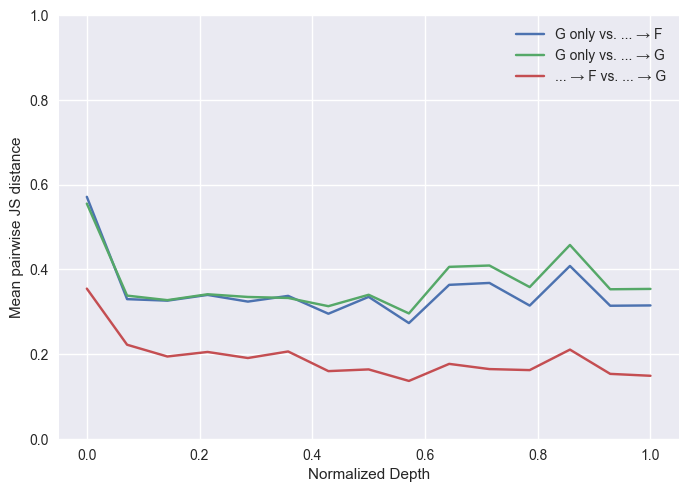
\includegraphics[width=\textwidth]{images/preliminary/jsd-depth-regg-indist.png}
        \caption{Regulation \textbf{G}, in-distribution ($n=1086$).}
        \label{fig:jsd-regg-indist}
    \end{subfigure}%
    \begin{subfigure}{.5\textwidth}
        \centering
        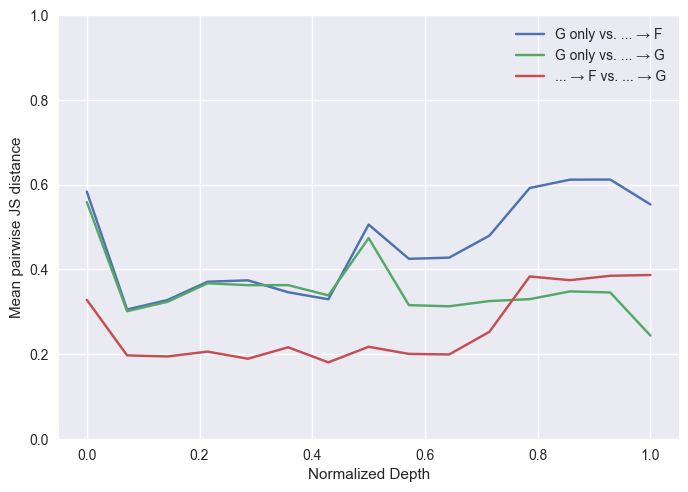
\includegraphics[width=\textwidth]{images/preliminary/jsd-depth-regg-outofdist.png}
        \caption{Regulation \textbf{G}, out-of-distribution ($n=1101$).}
        \label{fig:jsd-regg-outdist}
    \end{subfigure}
    \caption{Mean pairwise Jensen-Shannon distance between action probabilities for every observation, plotted against the normalized depth. Letters represent the regulation the agent is trained or fine-tuned on (e.g. ``$... \rightarrow \text{F}$" is fine-tuned from regulation \textbf{A} to \textbf{B} to ... to \textbf{F}).}
    \label{fig:jsd}
\end{figure}

Starting with the in-distribution results shown in Figures \ref{fig:jsd-regf-indist} and \ref{fig:jsd-regg-indist}, we can observe that the distance between the action probabilities of the two fine-tuned models (the red line) is consistently below the distance between the fine-tuned models and the model trained from scratch (the blue and green lines) for regulation \textbf{G}, while the three lines appear more balanced for regulation \textbf{F}.
Intuitively, this points towards a potential loss of plasticity in regulation \textbf{G}, keeping the fine-tuned model too similar in behavior to its source model and preventing it from fully adapting to regulation \textbf{G}.

Moving to the out-of-distribution results in Figures \ref{fig:jsd-regf-outdist} and \ref{fig:jsd-regg-outdist}, we can observe a similar trend in regulation \textbf{F} this time, although the differences are clearly smaller here.
In regulation \textbf{G} we can see a big shift compared to the other figures, especially for deeper observations.
While the red line stays below the other lines for most of the observations, we actually see the distance between the fine-tuned model and the model trained from scratch go below it near the end, suggesting that there is no loss of plasticity here.
This mixed result makes it difficult to draw concrete conclusions from this experiment.

In the next experiment we compare the value predictions of the agents when given the same observation.
We showed in Chapter \ref{sec:preliminary:finetune} that these agents have close to a 50\% win rate against each other, suggesting that we should expect to see value predictions centered around zero.
The results for this experiment, plotted against the normalized depth of the observation, can be found in Figure \ref{fig:value}.

\begin{figure}[H]
    \centering
    \begin{subfigure}{.5\textwidth}
        \centering
        
\includegraphics[width=\textwidth]{images/preliminary/value-regf-indist.png}
        \caption{Regulation \textbf{F}, in-distribution ($n=974$).}
        \label{fig:value-regf-indist}
    \end{subfigure}%
    \begin{subfigure}{.5\textwidth}
        \centering
        
\includegraphics[width=\textwidth]{images/preliminary/value-regf-outofdist.png}
        \caption{Regulation \textbf{F}, out-of-distribution ($n=1035$).}
        \label{fig:value-regf-outdist}
    \end{subfigure}
    \vskip\baselineskip
    \begin{subfigure}{.5\textwidth}
        \centering
        
\includegraphics[width=\textwidth]{images/preliminary/value-regg-indist.png}
        \caption{Regulation \textbf{G}, in-distribution ($n=1086$).}
        \label{fig:value-regg-indist}
    \end{subfigure}%
    \begin{subfigure}{.5\textwidth}
        \centering
        
\includegraphics[width=\textwidth]{images/preliminary/value-regg-outofdist.png}
        \caption{Regulation \textbf{G}, out-of-distribution ($n=1101$).}
        \label{fig:value-regg-outdist}
    \end{subfigure}
    \caption{Mean value prediction for every observation, plotted against the normalized depth. Letters represent the regulation the agent is trained or fine-tuned on (e.g. ``$... \rightarrow \text{F}$" is fine-tuned from regulation \textbf{A} to \textbf{B} to ... to \textbf{F}).}
    \label{fig:value}
\end{figure}

We can see in Figure \ref{fig:value} that the value predictions clearly do not fit our expectation of being centered around zero, instead showing quite unstable and inconsistent behavior.
The predictions shown in Figures \ref{fig:value-regf-indist}, \ref{fig:value-regf-outdist}, and \ref{fig:value-regg-outdist} show quite severe jumps, and in Figure \ref{fig:value-regf-indist} the mean value prediction of the model fine-tuned up to regulation \textbf{E} even drops below the minimum reward of -1 at some point.
These unexpected results make it difficult to conclude anything meaningful with regards to the transfer process, though there is an argument to be made that the value predictions of the model trained from scratch shows the least extreme behavior.
These results mainly raise further questions about the cause of these unstable value predictions, and their potential effect on the overall performance and transferability of the model.

The last experiment in this chapter involves the action logits computed by the agents.
We are interested in whether we can gain further insights into the transfer process by plotting the distribution of action logits using a t-SNE visualization.
We take the 256-dimensional action logits for each observation, reduce them to 50 dimensions using principal component analysis (PCA), then reduce them to two dimensions using t-SNE~\cite{van2008tsne}.
These visualizations can be found in Figure \ref{fig:tsne}.

\begin{figure}[H]
    \centering
    \begin{subfigure}{.5\textwidth}
        \centering
        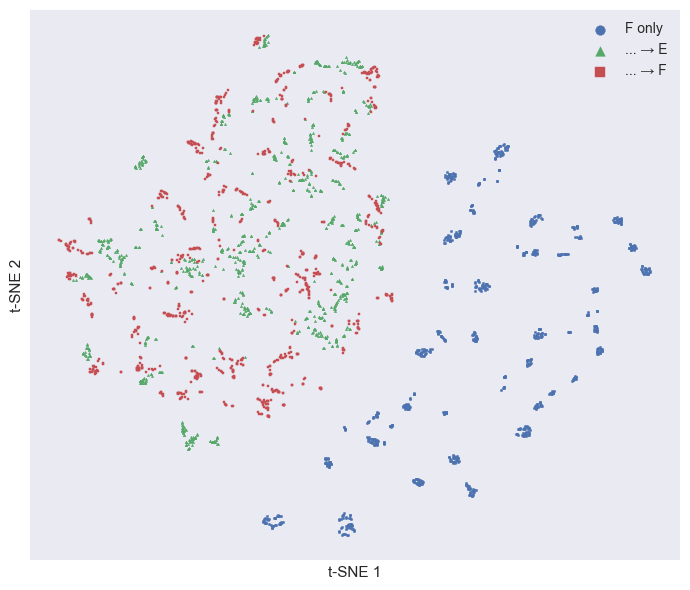
\includegraphics[width=\textwidth]{images/preliminary/tsne-regf-indist.png}
        \caption{Regulation \textbf{F}, in-distribution ($n=974$).}
        \label{fig:tsne-regf-indist}
    \end{subfigure}%
    \begin{subfigure}{.5\textwidth}
        \centering
        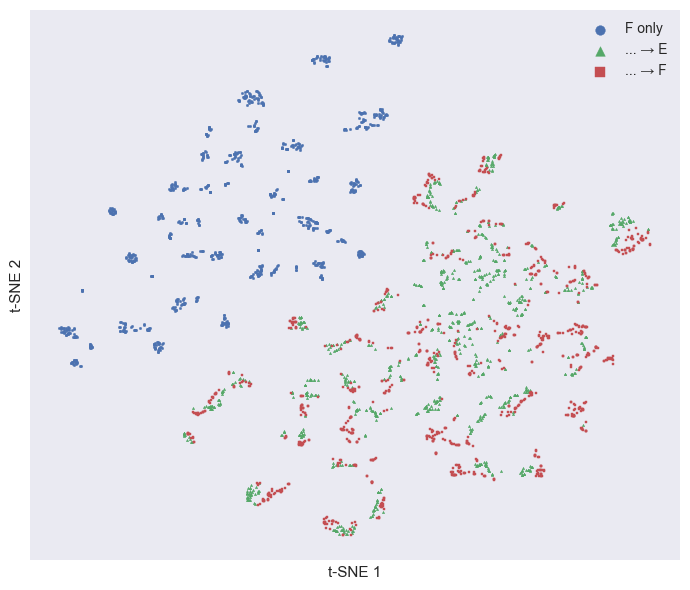
\includegraphics[width=\textwidth]{images/preliminary/tsne-regf-outofdist.png}
        \caption{Regulation \textbf{F}, out-of-distribution ($n=1035$).}
        \label{fig:tsne-regf-outdist}
    \end{subfigure}
    \vskip\baselineskip
    \begin{subfigure}{.5\textwidth}
        \centering
        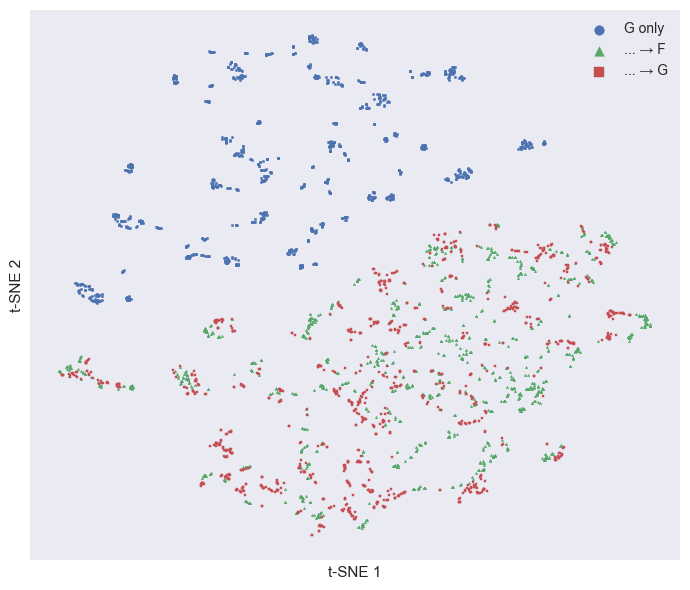
\includegraphics[width=\textwidth]{images/preliminary/tsne-regg-indist.png}
        \caption{Regulation \textbf{G}, in-distribution ($n=1086$).}
        \label{fig:tsne-regg-indist}
    \end{subfigure}%
    \begin{subfigure}{.5\textwidth}
        \centering
        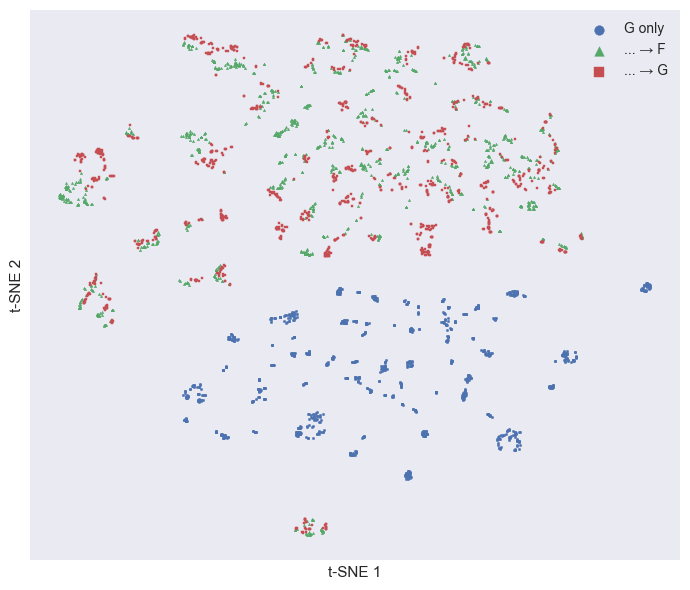
\includegraphics[width=\textwidth]{images/preliminary/tsne-regg-outofdist.png}
        \caption{Regulation \textbf{G}, out-of-distribution ($n=1101$).}
        \label{fig:tsne-regg-outdist}
    \end{subfigure}
    \caption{t-SNE visualization of action logits for every observation. Letters represent the regulation the agent is trained or fine-tuned on (e.g. ``$... \rightarrow \text{F}$" is fine-tuned from regulation \textbf{A} to \textbf{B} to ... to \textbf{F}).}
    \label{fig:tsne}
\end{figure}

A trend visible in Figure \ref{fig:tsne} is that the action logits of the model trained from scratch (the blue circles) appear to be distinguishable from the action logits of the models that are fine-tuned.
To get a clearer picture of the underlying structure, we sample 50 observations (150 points) from the above figures and connect points showing logits of the same observations.
Since t-SNE distorts global and local distances, we color these connecting lines according to the Jensen-Shannon distance between the action probabilities of the respective observations.
These visualizations can be found in Figure \ref{fig:tsne-lines}.

\begin{figure}[H]
    \centering
    \begin{subfigure}{.5\textwidth}
        \centering
        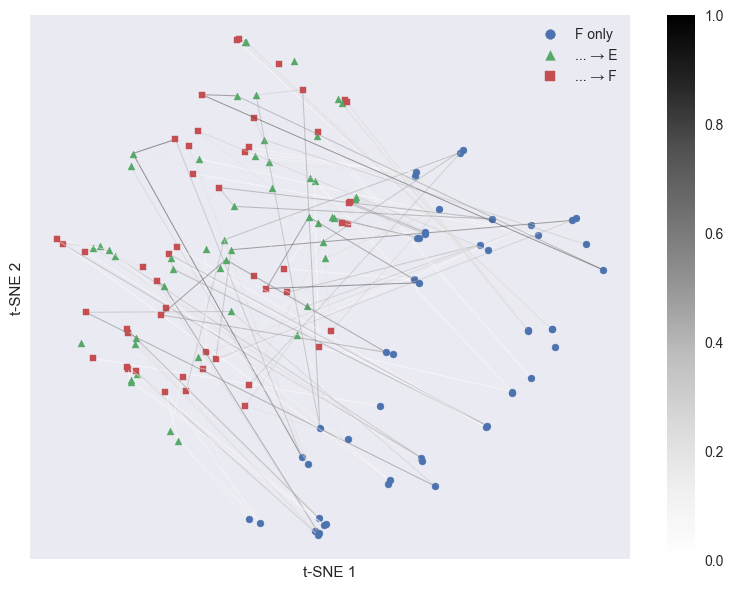
\includegraphics[width=\textwidth]{images/preliminary/tsne-regf-indist-lines.png}
        \caption{Regulation \textbf{F}, in-distribution.}
        \label{fig:tsne-regf-indist-lines}
    \end{subfigure}%
    \begin{subfigure}{.5\textwidth}
        \centering
        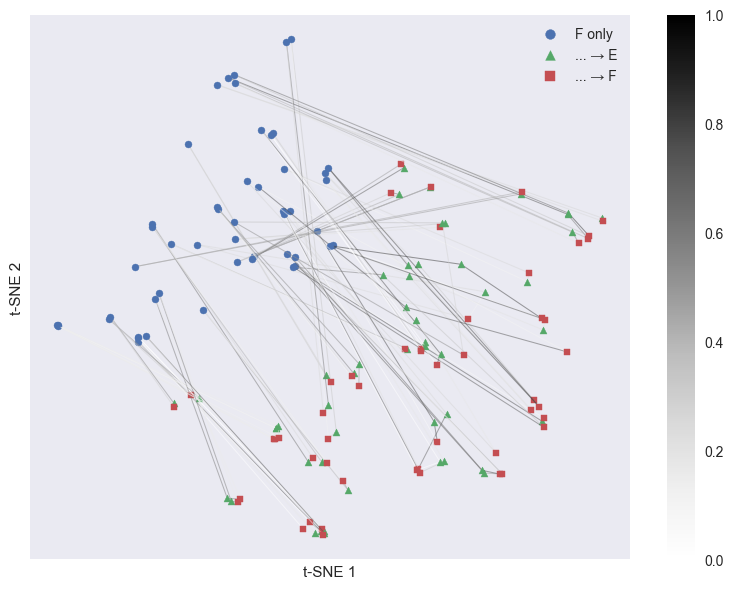
\includegraphics[width=\textwidth]{images/preliminary/tsne-regf-outofdist-lines.png}
        \caption{Regulation \textbf{F}, out-of-distribution.}
        \label{fig:tsne-regf-outdist-lines}
    \end{subfigure}
    \vskip\baselineskip
    \begin{subfigure}{.5\textwidth}
        \centering
        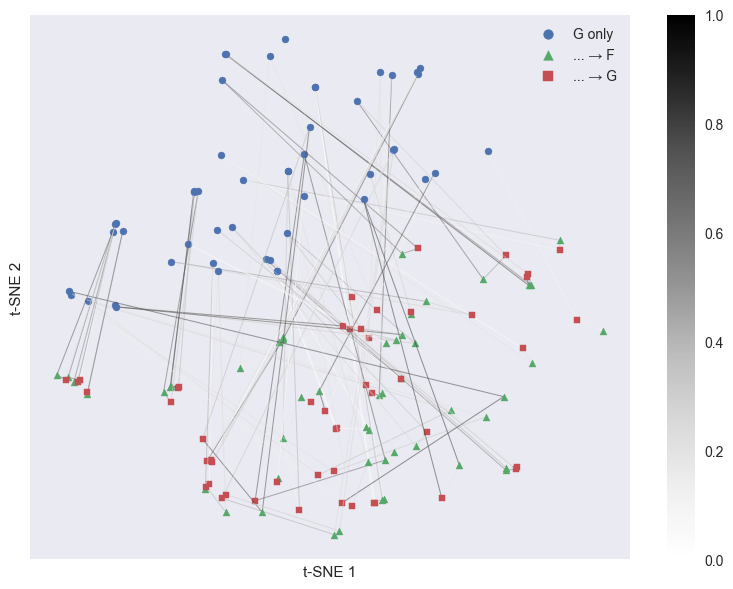
\includegraphics[width=\textwidth]{images/preliminary/tsne-regg-indist-lines.png}
        \caption{Regulation \textbf{G}, in-distribution.}
        \label{fig:tsne-regg-indist-lines}
    \end{subfigure}%
    \begin{subfigure}{.5\textwidth}
        \centering
        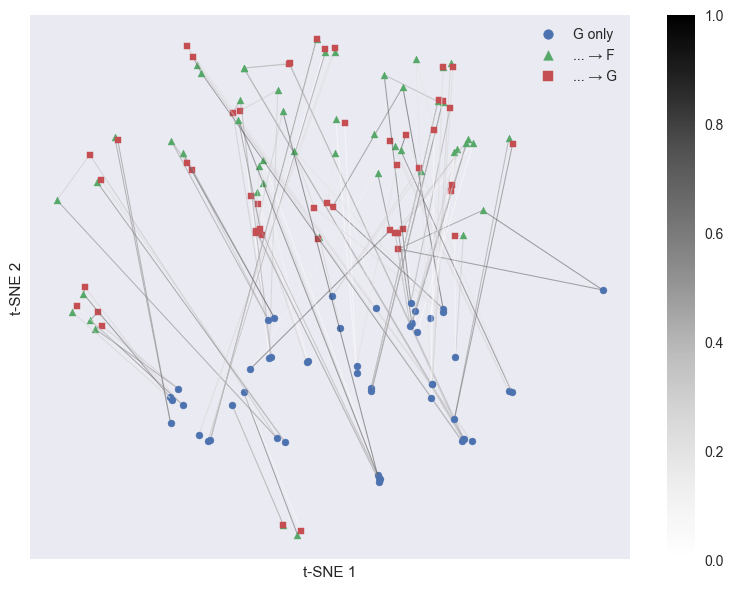
\includegraphics[width=\textwidth]{images/preliminary/tsne-regg-outofdist-lines.png}
        \caption{Regulation \textbf{G}, out-of-distribution.}
        \label{fig:tsne-regg-outdist-lines}
    \end{subfigure}
    \caption{t-SNE visualization of action logits for 50 sampled observations. Letters represent the regulation the agent in trained or fine-tuned on (e.g. ``$... \rightarrow \text{F}$" is fine-tuned from regulation \textbf{A} to \textbf{B} to ... to \textbf{F}). Lines connect points showing the same observation, and are colored according to the Jensen-Shannon distance between the respective action probabilities.}
    \label{fig:tsne-lines}
\end{figure}

Looking closely at Figure \ref{fig:tsne-lines}, we can observe that most of the action logits from the model trained from scratch (the blue circles) have dark lines at narrow, acute angles connecting them to the action logits of the other models.
This suggests that, generally speaking, the action logits and action probabilities of the two fine-tuned models stay closer to each other than to the model trained from scratch.
Similarly to the results shown in Figure \ref{fig:jsd}, this points towards the fine-tuned models potentially suffering from loss of plasticity.

\section{Conclusion} \label{sec:preliminary:conclusion}
Rounding up all the results of these preliminary experiments, we reflect back to the two questions posed at the beginning of this chapter:

\paragraph{1. What effect does non-stationarity have on the performance and generalization of reinforcement learning agents in VGC?}
We showed in Chapter \ref{sec:preliminary:transfer} that reinforcement learning agents are not capable of zero-shot transfer when evaluating using in-distribution teams.
When evaluating for generalization using out-of-distribution teams, the agents are capable of zero-shot transfer to future regulations, though there do exist outliers that will need further investigation.

\paragraph{2. To what extent are reinforcement learning agents able to maintain performance under non-stationarity without any continual learning techniques?}
We showed in Chapter \ref{sec:preliminary:finetune} that, in the best case, full fine-tuning can lead to positive transfer in the short term, but starts to lose out to complete retraining as the game moves further away from its initial definition.
Like before, we also observed multiple outliers here that will need further investigation.

Looking further into the behavior of the fine-tuned models in Chapter \ref{sec:preliminary:analysis}, we saw in Figures \ref{fig:jsd} and \ref{fig:tsne-lines} that the fine-tuned models are potentially held back by a loss of plasticity that causes them to stay too similar to their source model, preventing them from fully adapting to the new regulation.
We also observed unexpected and inconsistent behavior from the value function in Figure \ref{fig:value}, though it is unclear what effect this has on the performance, generalization, and transferability of the model.
We also have to acknowledge here that these experiments were only performed on one seed, making further experimentation necessary.

\newpage
%
% Methodology
%
\chapter{Methodology} \label{sec:methodology}
In this chapter we will propose several potential solutions to improve the performance of VGC-Bench's RL agents under non-stationarity.
We continue with the same problem statement and assumptions outlined in Chapter \ref{sec:preliminary}: We train an agent on regulation \textbf{A}, then on \textbf{B}, \textbf{C}, etc.
No regulation will be revisited after it is played, and no information about future regulations is available a priori.

Our first proposed improvement involves the policy architecture and the unstable behavior of the value function, as shown in Chapter \ref{sec:preliminary:analysis}.
While we initially used the same policy architecture as VGC-Bench (shown in Figure \ref{fig:vgcbench-architecture}), we now propose two minor adjustments to help stabilize the training of the value function:

\begin{enumerate}
    \item Change the Gaussian initialization of the item, move, and ability embeddings from $\mathcal{N}(0, 1)$ to $\mathcal{N}(0, 0.02)$. These embeddings receive sparse gradients, highly dependent on the items, moves, and abilities seen during training (with the majority never being seen at all). Additionally, these embeddings are suffering from vanishing gradients as they are placed at the very start of the network. Lowering the magnitude of the initialization makes the gradients more effective without drastically altering the original architecture. Despite this adjustment being in view of the value function, we apply this change to both the actor and the critic to keep their respective networks equivalent.
    \item Change the gain of the orthogonal initialization of the linear layer projecting the transformer output to the value prediction from 1 to 0.01. The large gain of the original initialization makes the initial value predictions biased and outside the $[-1, 1]$ range. Similarly to the embeddings, lowering the magnitude of the initialization reduces the effect of this bias and should make the learning of the value function more stable.
\end{enumerate}

With these two architectural adjustments to aid with the stability of the training process, we can now look into the various continual reinforcement learning methods outlined in Chapter \ref{sec:cl:crl}.

\textit{Regularization-based methods} identify parameters that are important for previously learned tasks and penalize changes to these parameters.
Alternatively, \textit{replay-based methods} store examples from previously encountered tasks and interleave them with new experiences during training.
While these methods could definitely have an impact in our problem setting, they are mainly focused on mitigating catastrophic forgetting and do not provide a clear solution to loss of plasticity~\cite{wang2024cl}.
Since in the scope of this thesis we explicitly state that no regulation will be revisited after it is played, we speculate that these methods will have less of an impact than methods that explicitly mitigate loss of plasticity.

\textit{Parameter-isolation methods} allocate separate subsets of model parameters to different tasks, providing a clear solution to loss of plasticity.
Progressive architectures like PNNs and PathNet are prime candidates for combining the plasticity of complete retraining with the knowledge retention of fine-tuning, though they will first have to be adapted to transformer models for VGC-Bench's policy architecture.
While LoRA is a compelling method that serves this purpose, it is more intended for large transformer models that cannot easily be fine-tuned, something that we already showed is possible for VGC-Bench's policy architecture in Chapter \ref{sec:preliminary:finetune}~\cite{hu2022lora}.

Other options for mitigating loss of plasticity include  specialized optimization methods like ReDo and Continual Backprop.
While these methods were explicitly created to combat loss of plasticity, recent work by \textcite{dohare2024plasticity} showed that they have a limited benefit over a tuned version of PPO in the context of continual reinforcement learning.
Combined with the fact that these methods have not yet been adapted for transformer models, we speculate that \textcite{dohare2024plasticity}'s tuned PPO will be able to give us more consistent results.

\section{Progressive Architecture} \label{sec:progressive}
Progressive neural networks are an established continual learning method that allocates separate 'columns' of a network to different tasks.
Each column has lateral connections to previous columns, allowing the network to reuse previously learned representations~\cite{rusu2016pnn}.
By introducing new weights for every task, PNNs effectively remove the issue of loss of plasticity.
For this reason, we believe that a progressive architecture could help improve the performance of VGC-Bench's RL agents under non-stationarity.

When adapting VGC-Bench's policy architecture to a progressive variant, we base our work on \textcite{rusu2016pnn}'s original PNN architecture, allocating separate columns for every regulation.
If network size becomes an issue we could consider switching to PathNet, an alternative to PNNs that operates on a fixed-size network~\cite{fernando2017pathnet}, but with only 10 regulations we do not foresee this becoming an issue.

\begin{figure}[ht]
    \centering
    \begin{subfigure}{.95\textwidth}
        \centering
        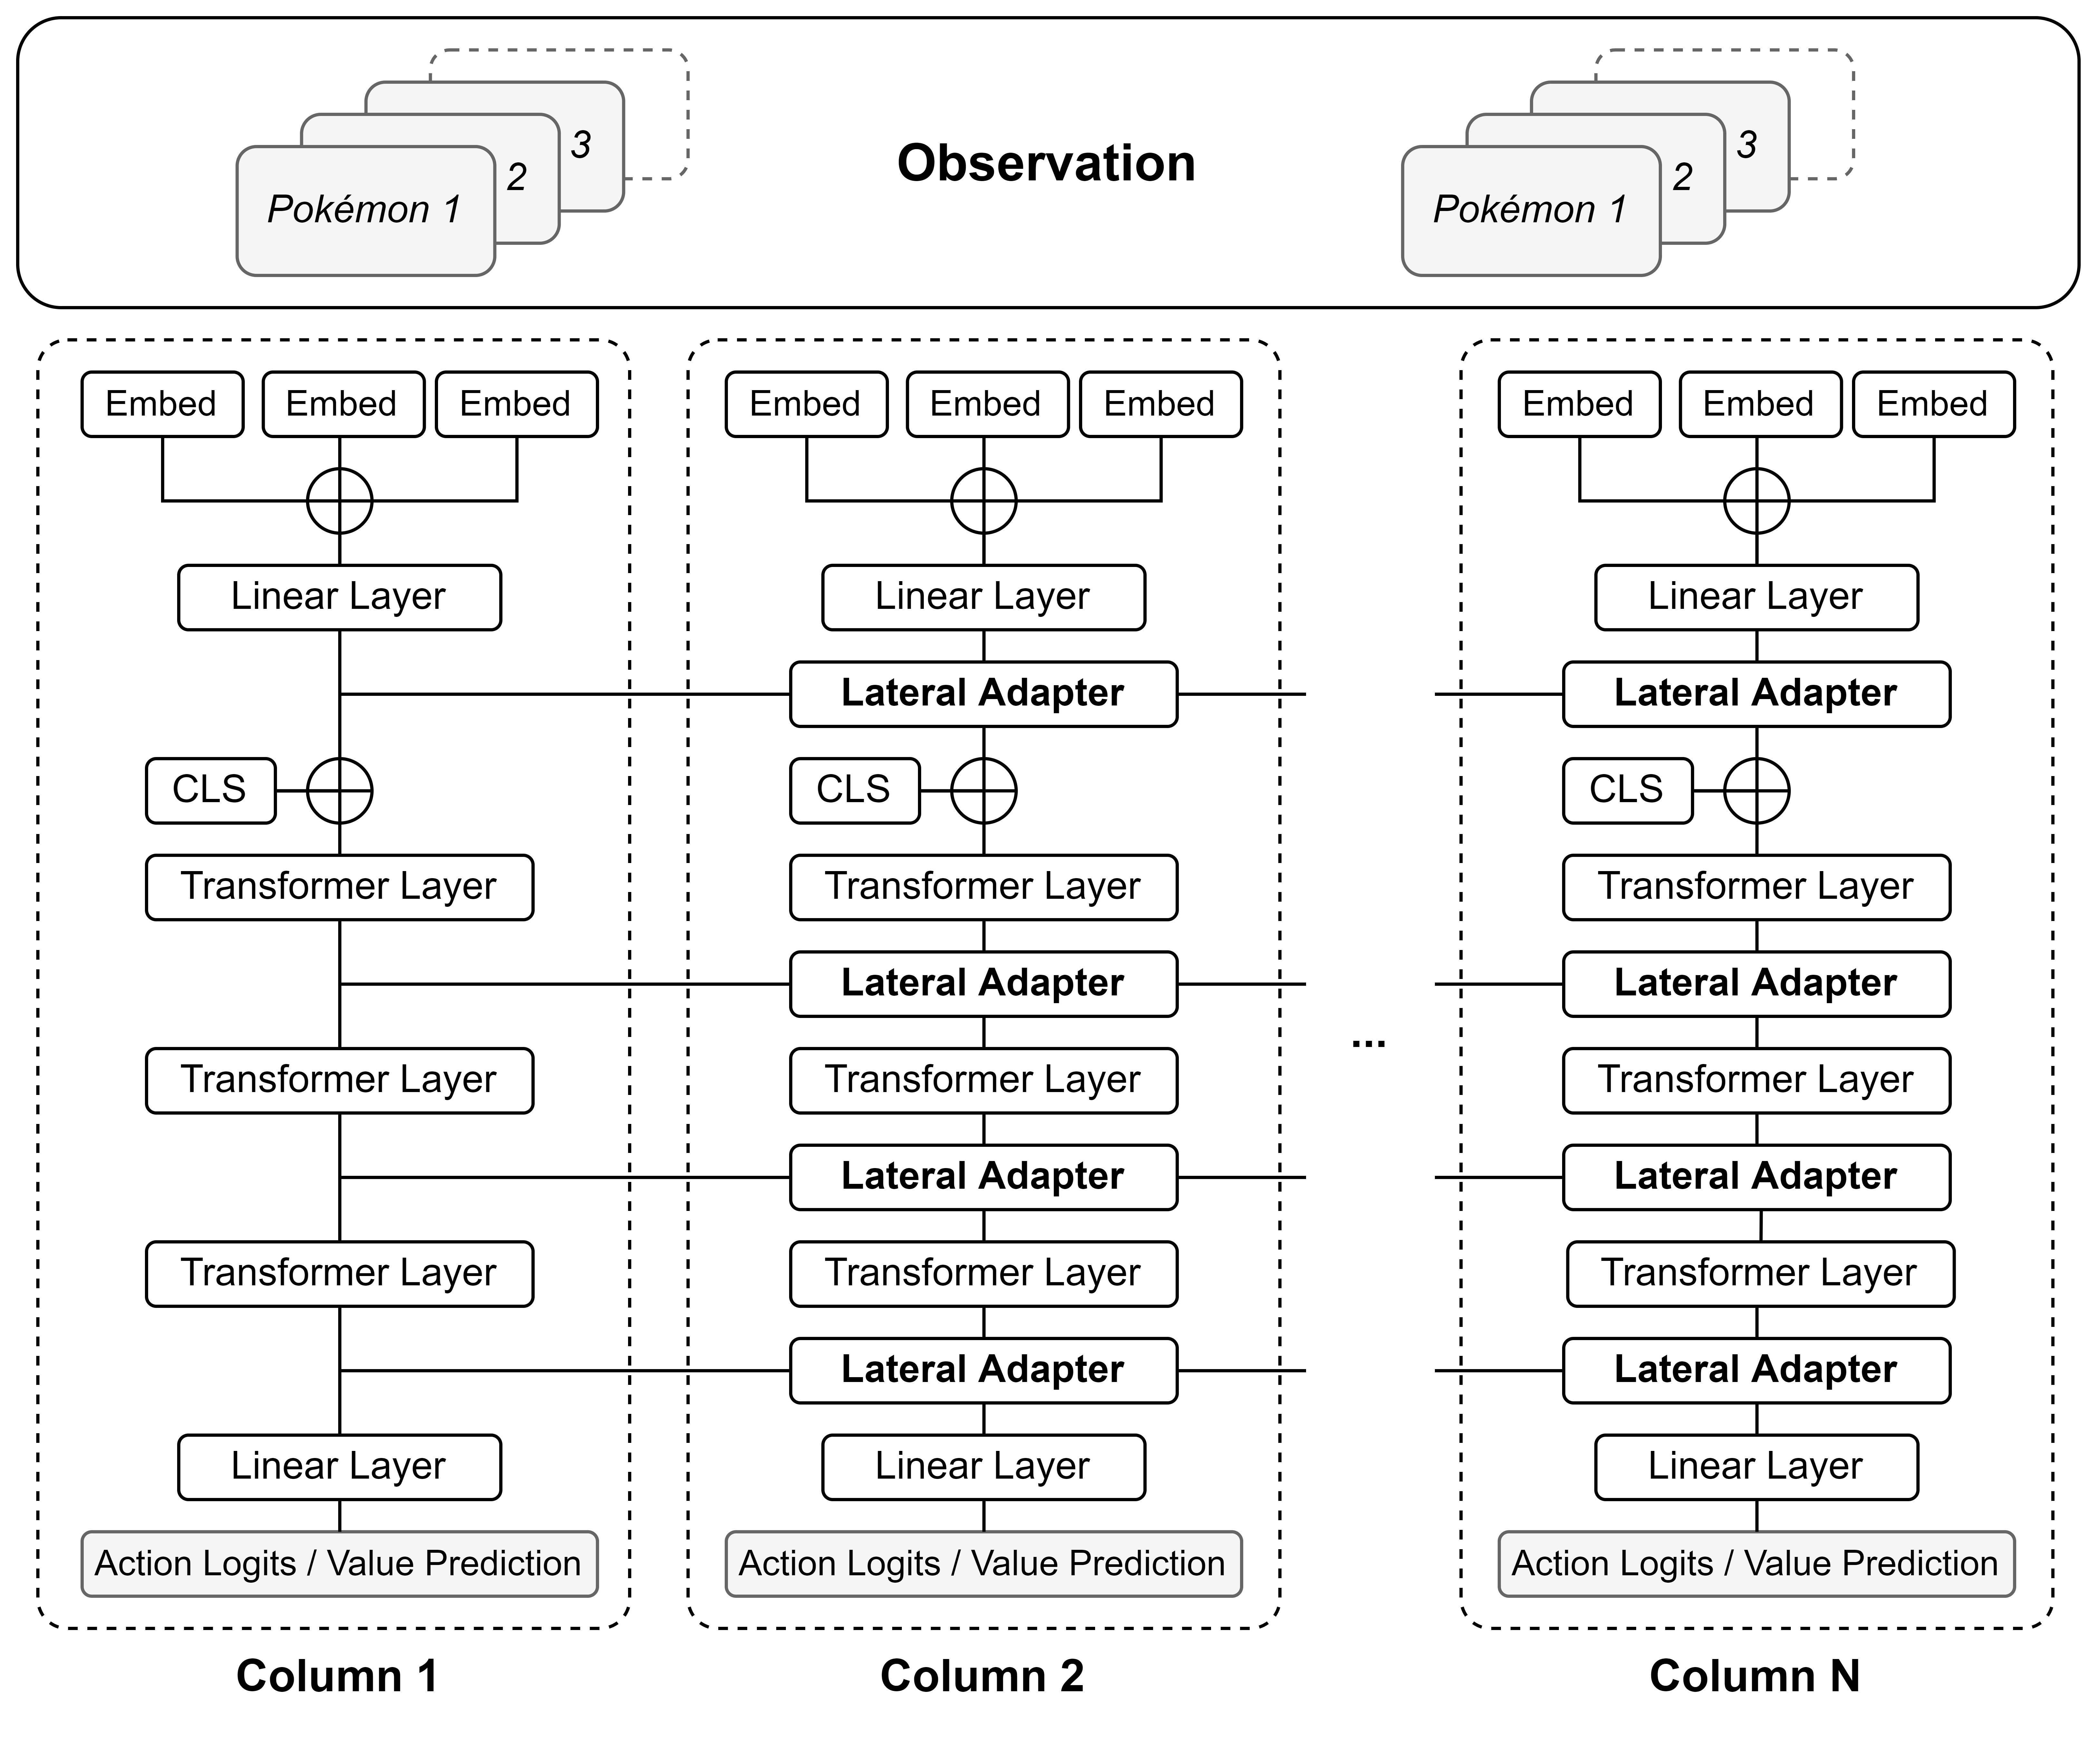
\includegraphics[width=\textwidth]{images/figures/progressive.png}
        \caption{Our proposed progressive architecture.}
        \label{fig:progressive:architecture}
    \end{subfigure}
    \par\bigskip
    \begin{subfigure}{.65\textwidth}
        \centering
        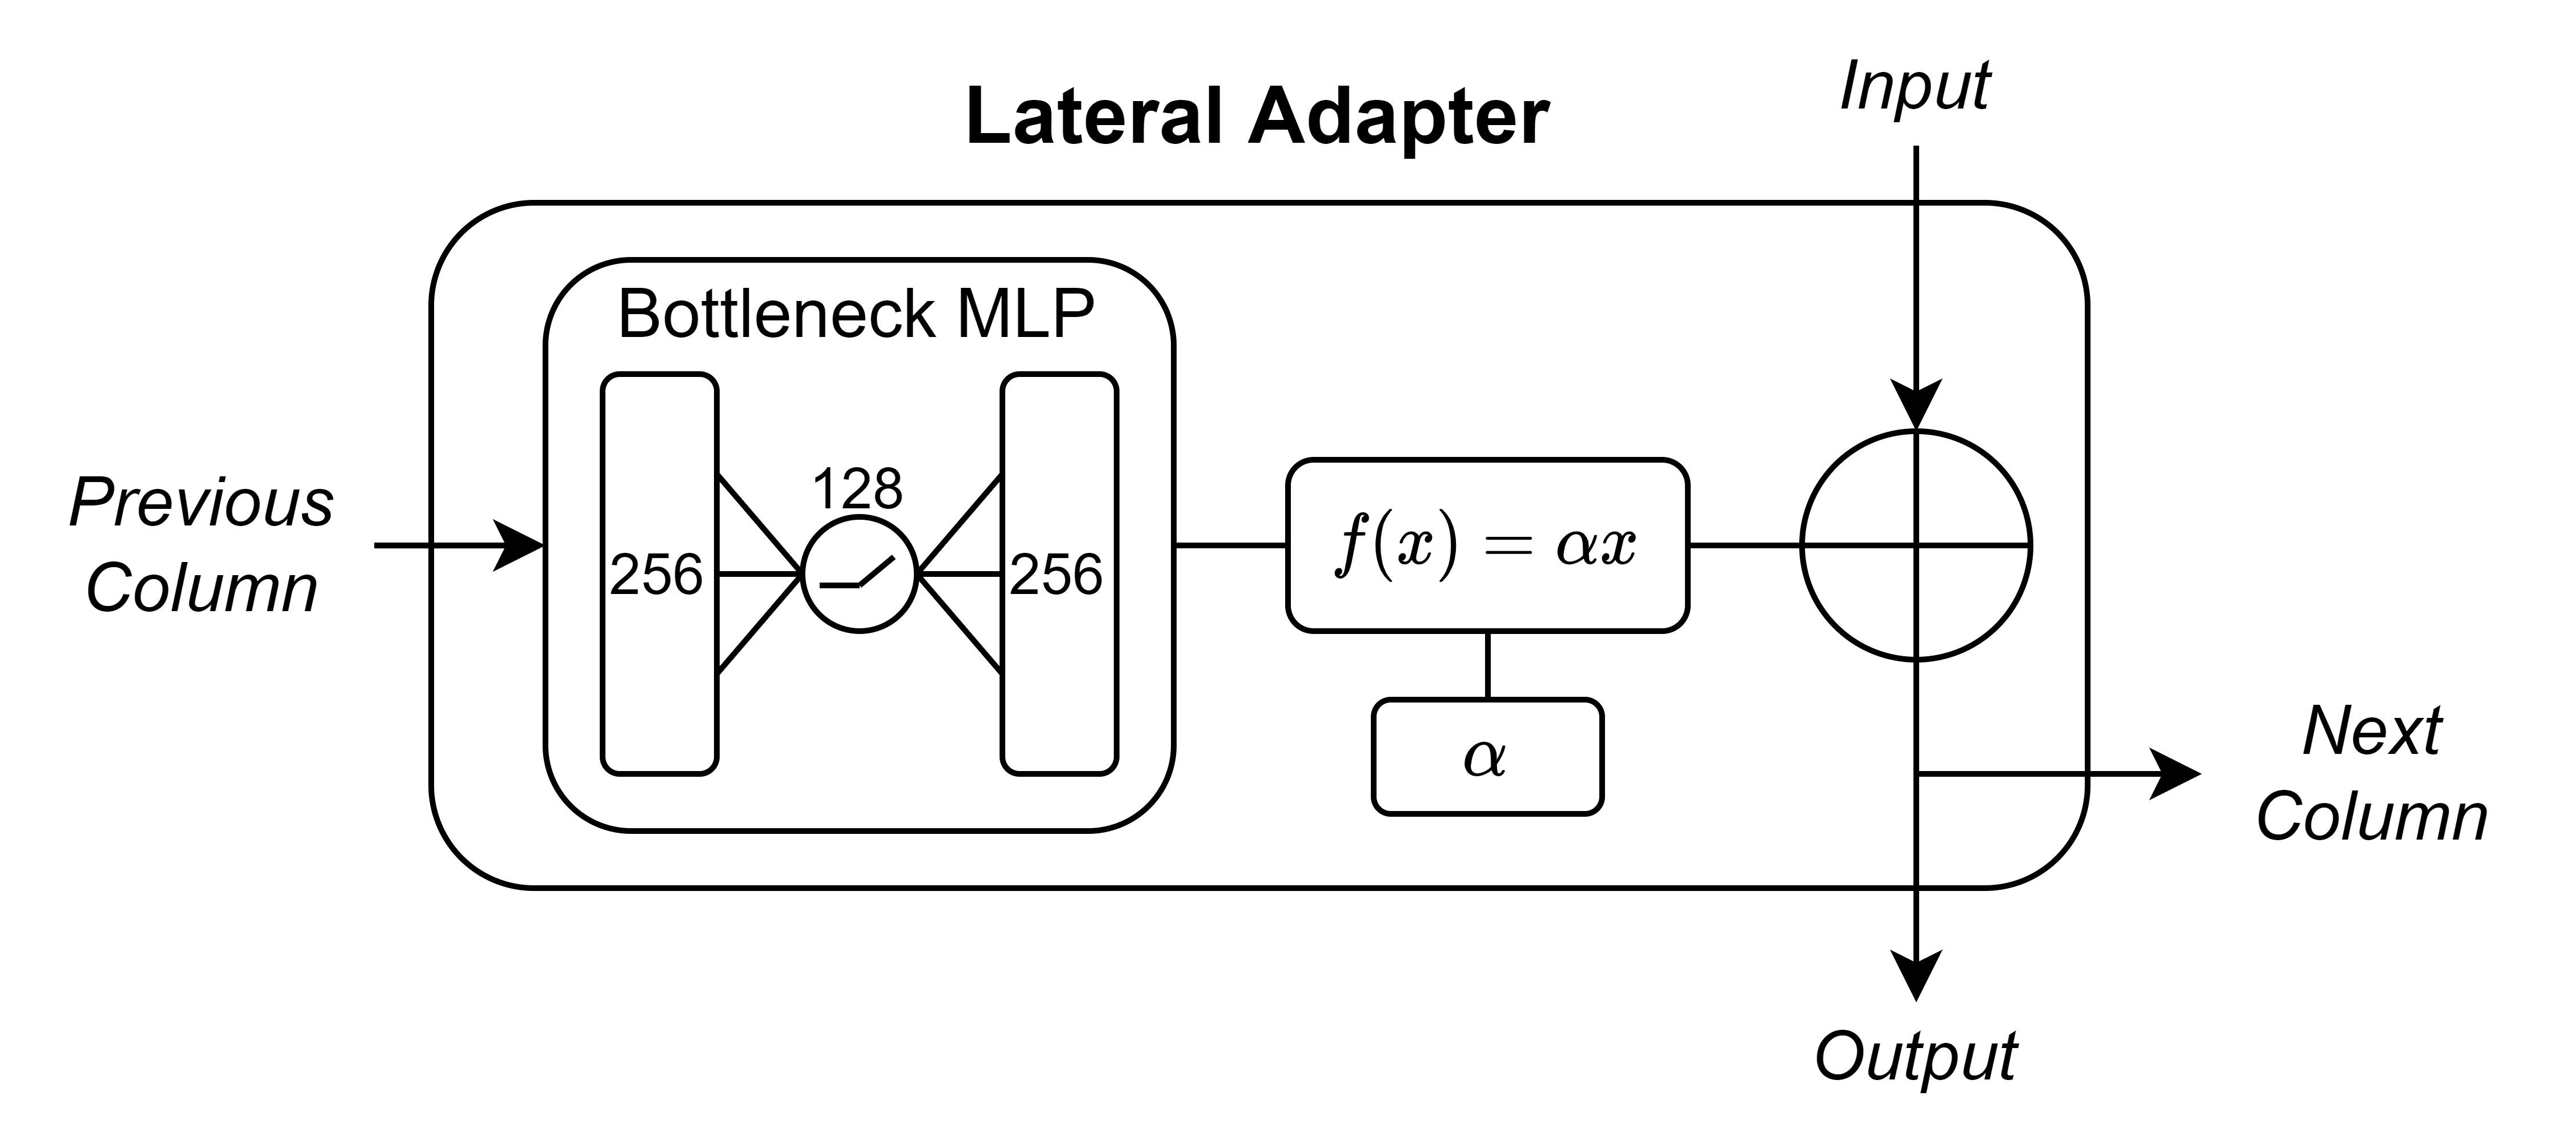
\includegraphics[width=\textwidth]{images/figures/lateral-adapter.png}
        \caption{The lateral adapter connecting adjacent columns.}
        \label{fig:progressive:adapter}
    \end{subfigure}
    \caption{VGC-Bench's policy architecture (see Figure \ref{fig:vgcbench-architecture}), adapted to a progressive variant with columns for regulations. Both actor and critic use the same architecture with separate columns and no direct parameter sharing.}
    \label{fig:progressive}
\end{figure}

Figure \ref{fig:progressive} shows our proposed adaptation of VGC-Bench's policy architecture to a progressive variant with columns for each regulation.
When a new column is added, the previous column's weights are frozen and stop receiving gradients.
We only use the action logits and value predictions of the column corresponding to the current regulation.
We identify four potential lateral transfer points: One after the feature aggregation, and one after each of the three transformer layers.
These transfer points feel closest in line to the original PNN architecture by \textcite{rusu2016pnn}, which transfers laterally after every network layer~\cite{rusu2016pnn}.

At each transfer point, the lateral signal from the previous column is combined with the current column's signal through a lateral adapter (shown in Figure \ref{fig:progressive:adapter}).
The lateral signal first passes through two linear layers arranged as a bottleneck, restricting the signal to half of its original dimensions and forcing it to a more robust representation.
It is then scaled by a learned vector $\alpha = (\alpha_1, \alpha_2, ... , \alpha_{256})$ before being added to the current column's signal.
This output signal is then passed to the rest of the current column or as lateral signal to the next column.

One adjustment we make compared to the original PNN architecture is that each column only provides a lateral signal to its next adjacent column, instead of all future columns~\cite{rusu2016pnn}.
This changes the growth of the network from exponential to linear, making it more compact while representations from column $i$ can still transfer to column $i + n$ through the cascading structure of lateral adapters.

\FloatBarrier

\section{Tuned PPO} \label{sec:tuned}
Rather than adapting specialized optimization methods like ReDo or Continual Backprop to transformer models, we are instead more interested in the tuned version of PPO, introduced by \textcite{dohare2024plasticity}, that achieves very similar results in continual reinforcement learning settings.

The main adjustment this tuned version makes is to the $\beta_1$ and $\beta_2$ parameters of the Adam optimizer, which relate to the optimizer's running estimate of the gradient and the squared gradient respectively.
The standard values of $\beta_1$ and $\beta_2$ used by the Adam optimizer (and PPO by extension) are 0.9 and 0.999 respectively.
\textcite{lyle2023plasticity} showed that these standard values cause a large loss of plasticity, caused by the fact that $\beta_1 \neq \beta_2$.
A large value of $\beta_2$ means that the running estimate for the squared gradient, used in the denominator, is updated much more slowly than the running estimate for the gradient, used in the numerator~\cite{dohare2024plasticity,lyle2023plasticity}.
\textcite{lyle2023plasticity} proposed setting $\beta_1 = \beta_2 = 0.99$, resulting in smaller updates that lead to a more stable training.

\textcite{dohare2024plasticity} used this tuned version of the Adam optimizer combined with PPO and L2 regularization as a baseline for ReDo and Continual Backprop in a continual reinforcement learning setting, referring to it as \textit{``tuned PPO"}.
While tuned PPO performed worse than Continual Backprop in stationary environments, it was able to keep up in non-stationarity environments, only falling 1-2\% percent behind in terms of reward while vastly outperforming regular PPO~\cite{dohare2024plasticity}.
For this reason, we believe that tuned PPO could help improve the performance of VGC-Bench's RL agents under non-stationarity.

We replicate \textcite{dohare2024plasticity}'s tuned PPO by updating the Adam optimizer's $\beta$'s to $\beta_1 = \beta_2 = 0.99$ and by enabling L2 regularization, both for training and for fine-tuning.
The only adjustment we make has to do with the L2 regularization rate $\lambda$: Whereas \textcite{dohare2024plasticity} use a rate of 1e-5, we opt for a more conservative 1e-6.

\newpage
%
% Experiments
%
\chapter{Experiments} \label{sec:experiments}
In this chapter we will perform experiments to investigate to what extent the methods proposed in Chapter \ref{sec:methodology} can improve the performance of VGC-Bench's RL agents under non-stationarity.
We do this in three phases:

\begin{enumerate}
    \item \textbf{Stationary Experiments:} We train progressive and tuned PPO agents from scratch on each regulation and evaluate using 1000 episodes of cross-play, both in-distribution and out-of-distribution, against the original VGC-Bench RL agents. This experiment will show us what effect a progressive architecture and tuned PPO have on the performance and generalization of agents in a stationary environment.
    \item \textbf{Non-Stationary Experiments:} We transfer the agents trained on regulation \textbf{A} to regulation \textbf{B}, then \textbf{C}, etc. using the progressive architecture, full fine-tuning using tuned PPO, and a combination of the two. We evaluate using 1000 episodes of cross-play, both in-distribution and out-of-distribution, against the original fine-tuned agents and agents trained from scratch. This experiment will show us what effect a progressive architecture and tuned PPO have on the performance and generalization of agents in a non-stationary setting.
    \item \textbf{Analysis Experiments:} To further analyze the effects of a progressive architecture and tuned PPO, we will also repeat the action probabilities, value function, and action logits experiments performed in Chapter \ref{sec:preliminary:analysis}.
\end{enumerate}

All agents are implemented as outlined in Chapter \ref{sec:methodology} and trained using the default hyperparameters shown in Table \ref{tab:hyperparam-vgcbench}, unless otherwise stated.
Just as in Chapter \ref{sec:preliminary}, regulations \textbf{B}, \textbf{E}, and \textbf{J} are excluded from out-of-distribution results because there are not enough teams available for a full out-of-distribution set.

\section{Stationary Results} \label{sec:results:stationary}
We train progressive and tuned PPO agents on all regulations.
Evaluation is done, both in-distribution and out-of-distribution, using 1000 episodes of cross-play against each other and against the original, unmodified VGC-Bench agents.
The results are shown in Figure \ref{fig:stationary}.

\begin{figure}[H]
    \centering
    \begin{subfigure}{\textwidth}
        \centering
        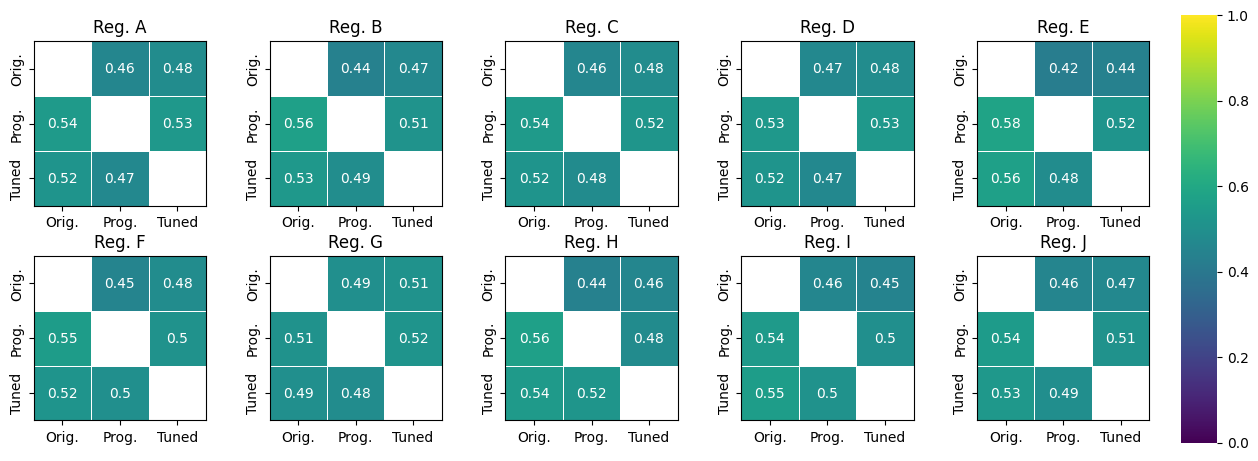
\includegraphics[width=\textwidth]{images/experiments/stationary-indist.png}
        \caption{In-distribution.}
        \label{fig:stationary-indist}
    \end{subfigure}
    \par\bigskip
    \begin{subfigure}{.85\textwidth}
        \centering
        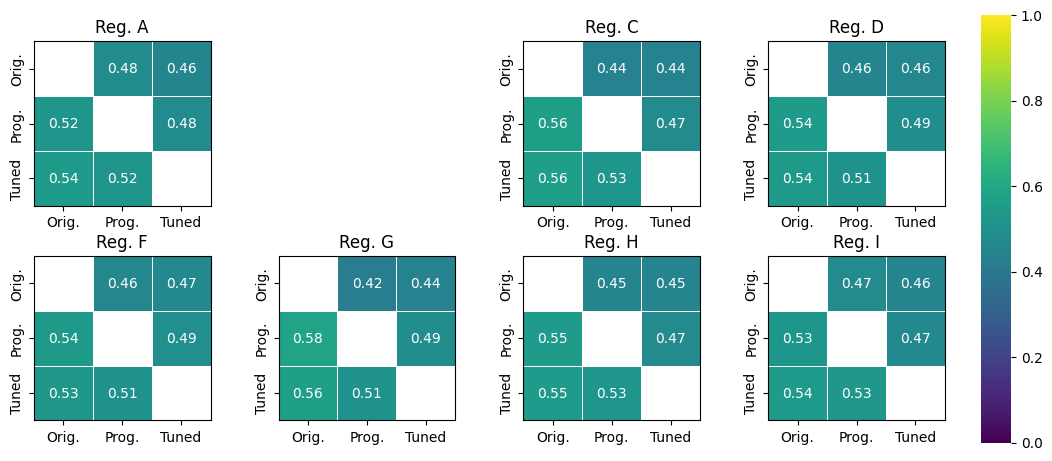
\includegraphics[width=\textwidth]{images/experiments/stationary-outofdist.png}
        \caption{Out-of-distribution.}
        \label{fig:stationary-outdist}
    \end{subfigure}
    \caption{Win rates of the row player over 1000 episodes in each regulation. \textit{``Orig."} refers to the original, unmodified agents from VGC-Bench, \textit{``Prog."} refers to agents trained with a progressive architecture, \textit{``Tuned"} refers to agents trained using tuned PPO.}
    \label{fig:stationary}
\end{figure}

We define our null hypothesis $H_0$ to be that an agent $\phi$ is equally skilled or worse than an agent $\psi$, and we define our significance level to be $\alpha=0.05$.
Just as in Chapter \ref{sec:preliminary}, we use a Binomial test with $n=1000$ and an expected win rate of $p \leq 0.5$ to calculate the p-values of the win rates of agent $\phi$.
These p-values are shown in Figure \ref{fig:stationary-pvalues}.

\begin{figure}[H]
    \centering
    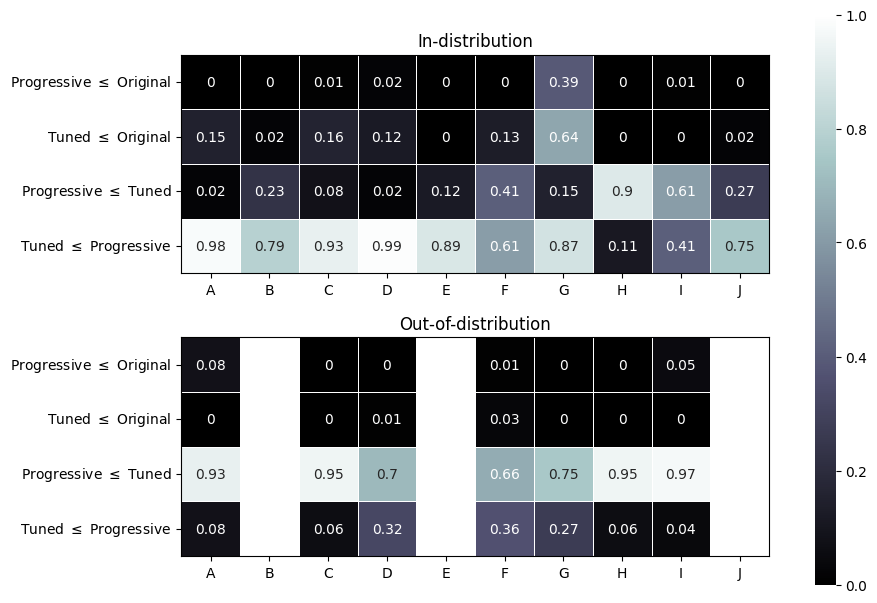
\includegraphics[width=0.9\textwidth]{images/experiments/stationary-pvalues.png}
    \caption{P-values of the win rates of the left agent against the right agent (e.g. the top row shows the p-values of the win rates of the agent with a progressive architecture against the original agent, belonging to the null hypothesis that the former is equally skilled or worse than the latter). Letters on the horizontal axis represent the regulation the agents are trained and evaluated on.}
    \label{fig:stationary-pvalues}
\end{figure}

\section{Non-Stationary Results} \label{sec:results:nonstationary}
We transfer the agents trained on regulation \textbf{A} to regulation \textbf{B}, then \textbf{C}, etc. using the progressive architecture (\textit{``progressive agents"}), full fine-tuning using tuned PPO (\textit{``tuned agents"}), and a combination of both (\textit{``combined agents"}).
Additional training or fine-tuning is always done for the same number of steps as training from scratch to provide an upper bound of the expected performance, and using the same hyperparameters as regular training (excluding tuned PPO, as outlined in Chapter \ref{sec:tuned}).
We evaluate using 1000 episodes of cross-play, both in-distribution and out-of-distribution, against the original fine-tuned agents and agents trained from scratch.

The results for the progressive, tuned, and combined agents are shown in Figures \ref{fig:progressive-experiments}, \ref{fig:tuned-experiments}, and \ref{fig:combined-experiments} respectively.
Additionally, results showing how the three types of agents compare against each other are shown in Figure \ref{fig:compared-experiments}.
Using the same null hypothesis, significance level, and statistical test as in Chapter \ref{sec:results:stationary}, the p-values of the win rates of the progressive, tuned, and combined agents are shown in Figures \ref{fig:progressive-pvalues}, \ref{fig:tuned-pvalues}, and \ref{fig:combined-pvalues} respectively.

\begin{figure}[ht]
    \centering
    \begin{subfigure}{.5\textwidth}
        \centering
        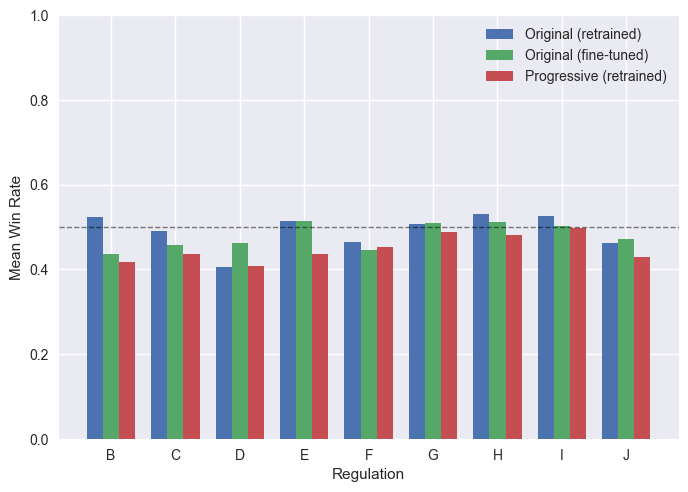
\includegraphics[width=\textwidth]{images/experiments/progressive-indist.png}
        \caption{In-distribution.}
        \label{fig:progressive-indist}
    \end{subfigure}%
    \begin{subfigure}{.5\textwidth}
        \centering
        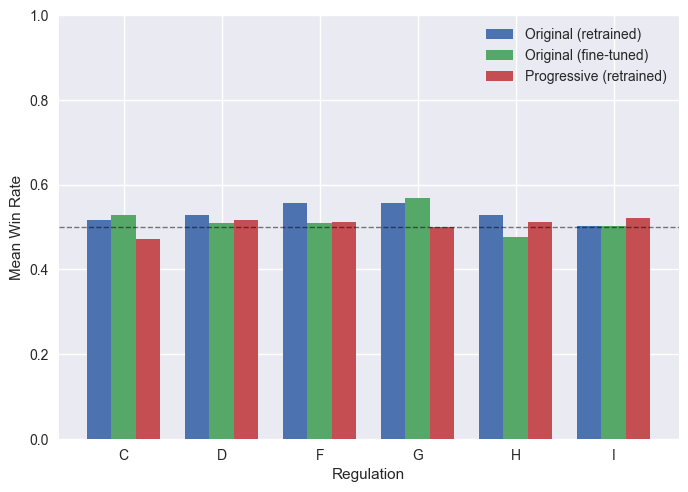
\includegraphics[width=\textwidth]{images/experiments/progressive-outofdist.png}
        \caption{Out-of-distribution.}
        \label{fig:progressive-outofdist}
    \end{subfigure}
    \caption{Mean win rates of progressive agents against VGC-Bench's original agents trained from scratch (blue), VGC-Bench's original agents fine-tuned (green), and progressive agents trained from scratch (red). Evaluated over 1000 episodes on each regulation.}
    \label{fig:progressive-experiments}
\end{figure}

\begin{figure}[ht]
    \centering
    \begin{subfigure}{.5\textwidth}
        \centering
        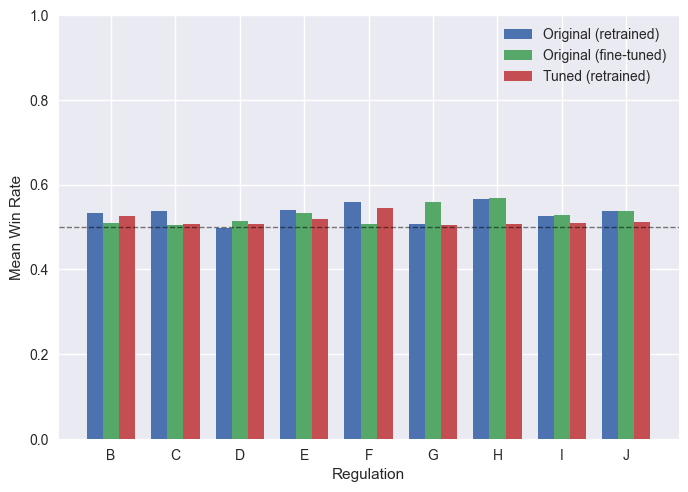
\includegraphics[width=\textwidth]{images/experiments/tuned-indist.png}
        \caption{In-distribution.}
        \label{fig:tuned-indist}
    \end{subfigure}%
    \begin{subfigure}{.5\textwidth}
        \centering
        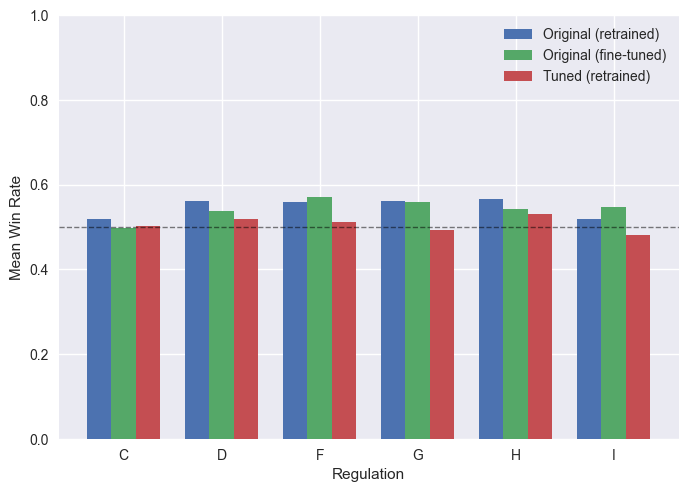
\includegraphics[width=\textwidth]{images/experiments/tuned-outofdist.png}
        \caption{Out-of-distribution.}
        \label{fig:tuned-outofdist}
    \end{subfigure}
    \caption{Mean win rates of tuned agents against VGC-Bench's original agents trained from scratch (blue), VGC-Bench's original agents fine-tuned (green), and tuned agents trained from scratch (red). Evaluated over 1000 episodes on each regulation.}
    \label{fig:tuned-experiments}
\end{figure}

\begin{figure}[ht]
    \centering
    \begin{subfigure}{.5\textwidth}
        \centering
        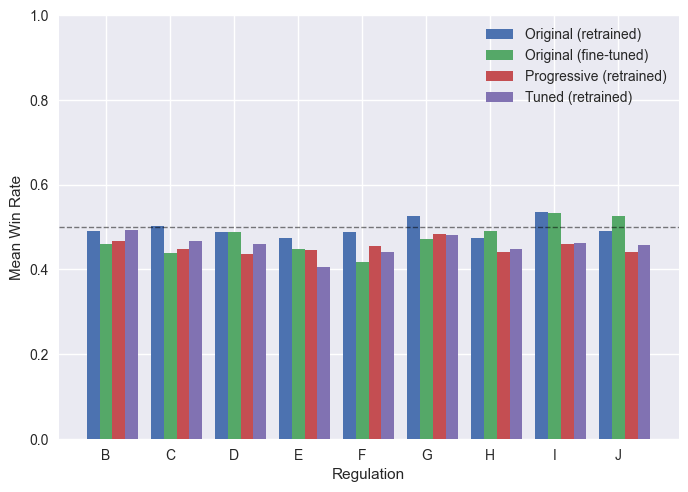
\includegraphics[width=\textwidth]{images/experiments/combined-indist.png}
        \caption{In-distribution.}
        \label{fig:combined-indist}
    \end{subfigure}%
    \begin{subfigure}{.5\textwidth}
        \centering
        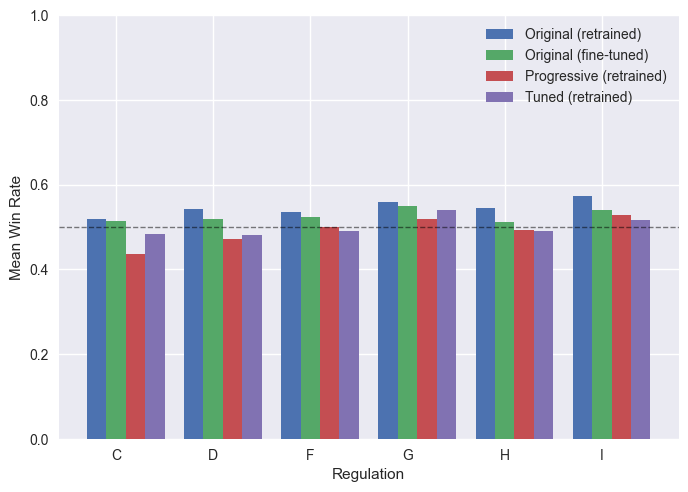
\includegraphics[width=\textwidth]{images/experiments/combined-outofdist.png}
        \caption{Out-of-distribution.}
        \label{fig:combined-outofdist}
    \end{subfigure}
    \caption{Mean win rates of combined agents against VGC-Bench's original agents trained from scratch (blue), VGC-Bench's original agents fine-tuned (green), progressive agents trained from scratch (red), and tuned agents trained from scratch (purple). Evaluated over 1000 episodes on each regulation.}
    \label{fig:combined-experiments}
\end{figure}

\begin{figure}[ht]
    \centering
    \begin{subfigure}{0.9\textwidth}
        \centering
        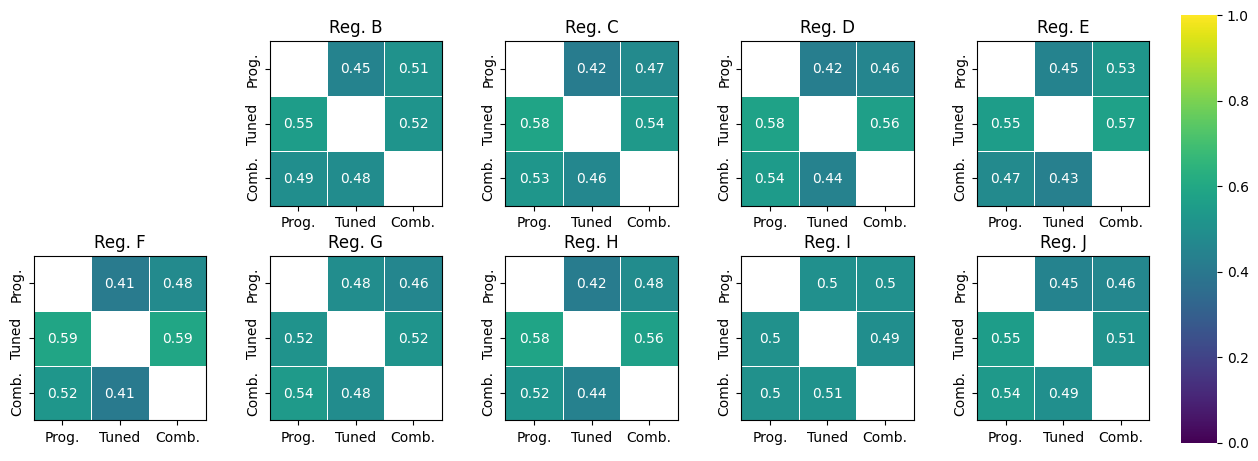
\includegraphics[width=\textwidth]{images/experiments/compared-indist.png}
        \caption{In-distribution.}
        \label{fig:compared-indist}
    \end{subfigure}
    \par\bigskip
    \begin{subfigure}{.55\textwidth}
        \centering
        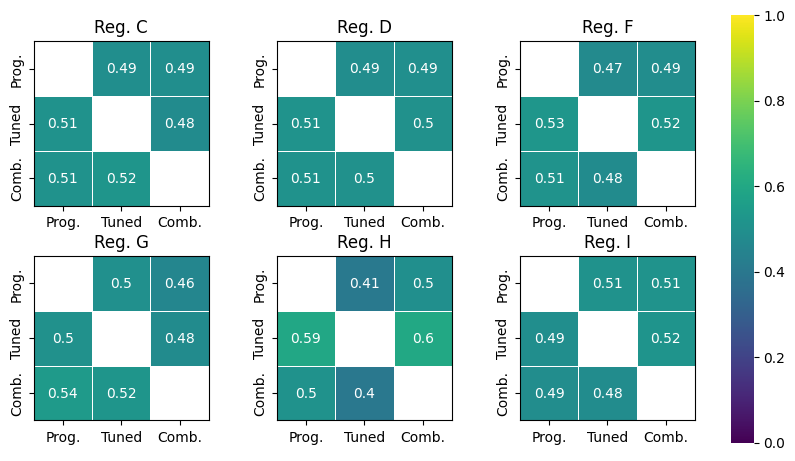
\includegraphics[width=\textwidth]{images/experiments/compared-outofdist.png}
        \caption{Out-of-distribution.}
        \label{fig:compared-outdist}
    \end{subfigure}
    \caption{Win rates of the row player over 1000 episodes in each regulation. \textit{``Prog."} refers to progressive agents, \textit{``Tuned"} refers to tuned agents, \textit{``Comb."} refers to combined agents.}
    \label{fig:compared-experiments}
\end{figure}

\begin{figure}[ht]
    \centering
    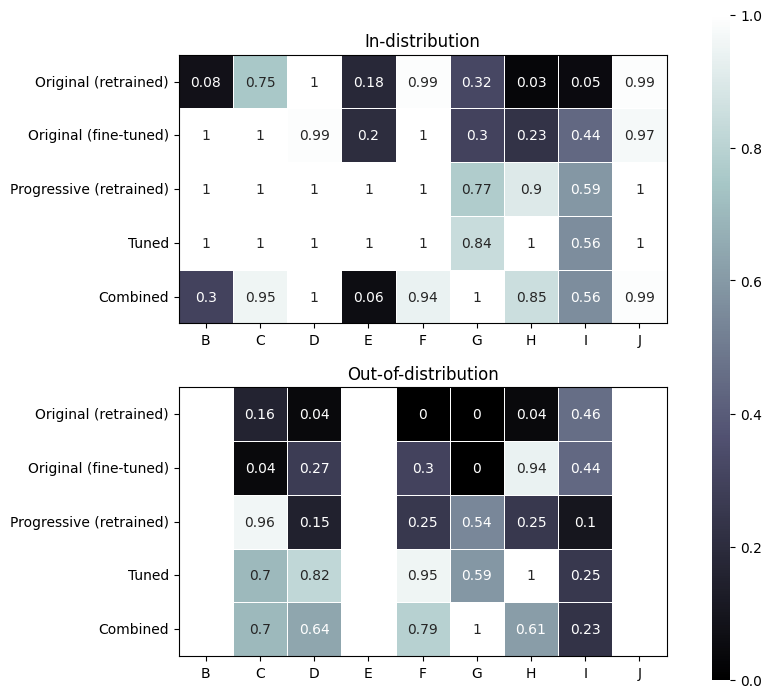
\includegraphics[width=\textwidth]{images/experiments/progressive-pvalues.png}
    \caption{P-values of the win rates of progressive agents against the agents on the vertical axis, in the regulation on the horizontal axis.}
    \label{fig:progressive-pvalues}
\end{figure}

\begin{figure}[ht]
    \centering
    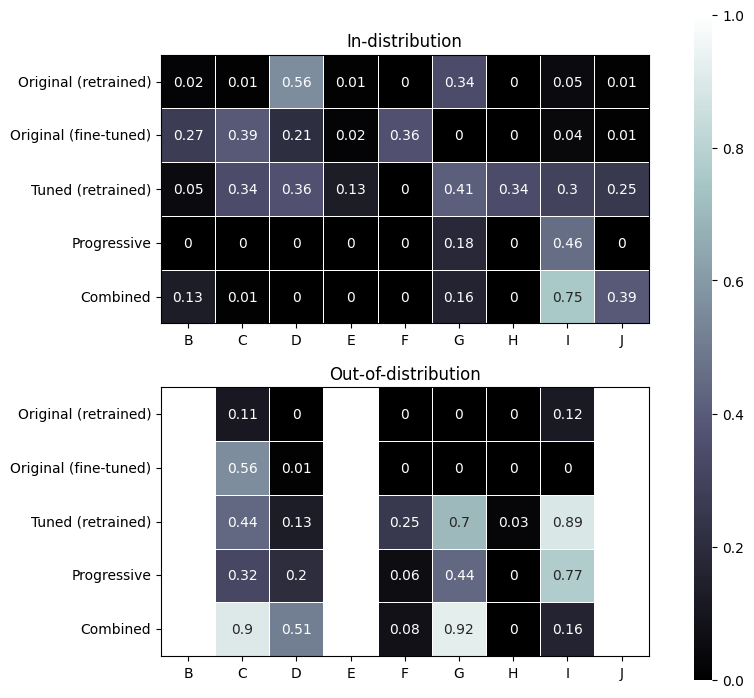
\includegraphics[width=\textwidth]{images/experiments/tuned-pvalues.png}
    \caption{P-values of the win rates of the tuned agents against the agents on the vertical axis, in the regulation on the horizontal axis.}
    \label{fig:tuned-pvalues}
\end{figure}

\begin{figure}[ht]
    \centering
    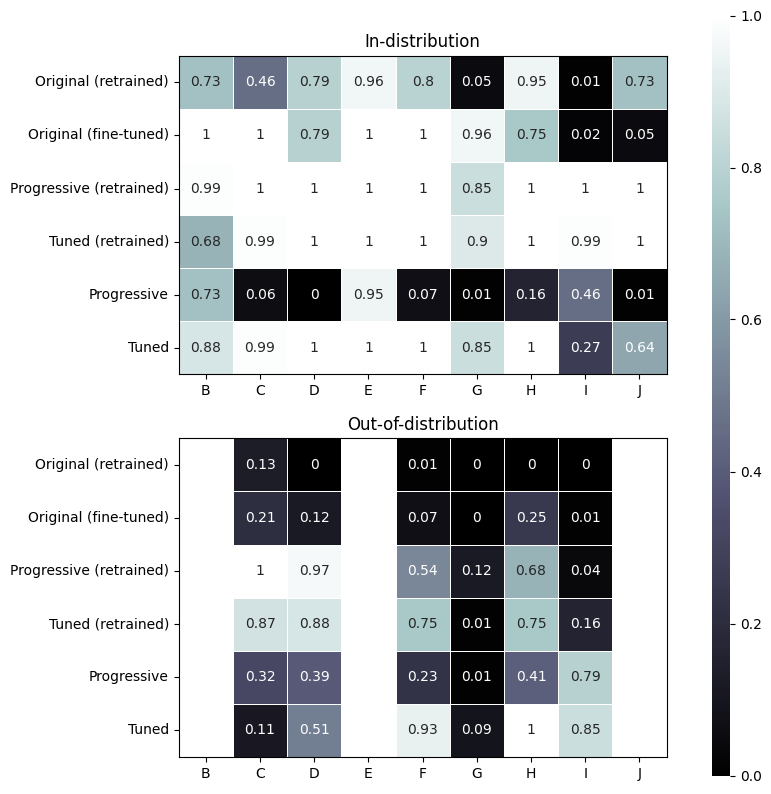
\includegraphics[width=\textwidth]{images/experiments/combined-pvalues.png}
    \caption{P-values of the win rates of the combined agents against the agents on the vertical axis, in the regulation on the horizontal axis.}
    \label{fig:combined-pvalues}
\end{figure}

\FloatBarrier

\section{Analysis Results} \label{sec:results:analysis}
Just as in Chapter \ref{sec:preliminary:analysis}, we further analyze our agents in regulations \textbf{F} and \textbf{G} by running 100 episodes of cross-play, both in-distribution and out-of-distribution, collecting statistics such as action probabilities, action logits, and value predictions for every observation.
We do this for the progressive agent trained on the regulation from scratch, the progressive and tuned agents fine-tuned up to the regulation, and the progressive and tuned agents fine-tuned up to the previous regulation.
We omit the combined agent from these experiments as we are more interested in analyzing the methods individually.

The first experiment focuses on how similar the agents are in their decision making, which we measure as the Jensen-Shannon distance between their respective action probabilities.
The results are shown in Figure \ref{fig:jsd-experiments}.

\begin{figure}[H]
    \centering
    \begin{subfigure}{.475\textwidth}
        \centering
        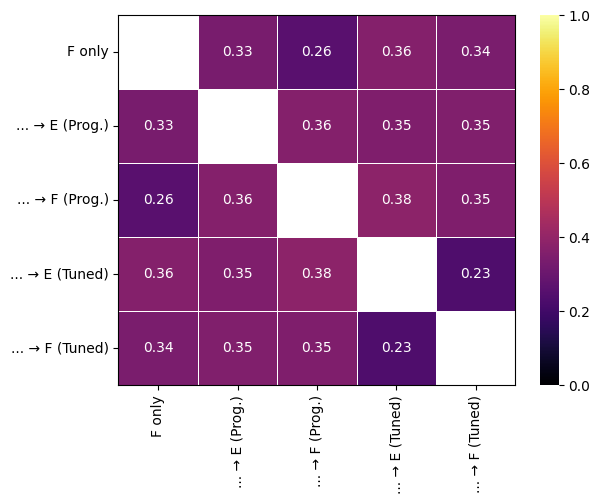
\includegraphics[width=\textwidth]{images/experiments/jsd-regf-indist.png}
        \caption{Regulation \textbf{F}, in-distribution ($n=924$).}
        \label{fig:jsd-experiments-regf-indist}
    \end{subfigure}
    \hfill
    \begin{subfigure}{.475\textwidth}
        \centering
        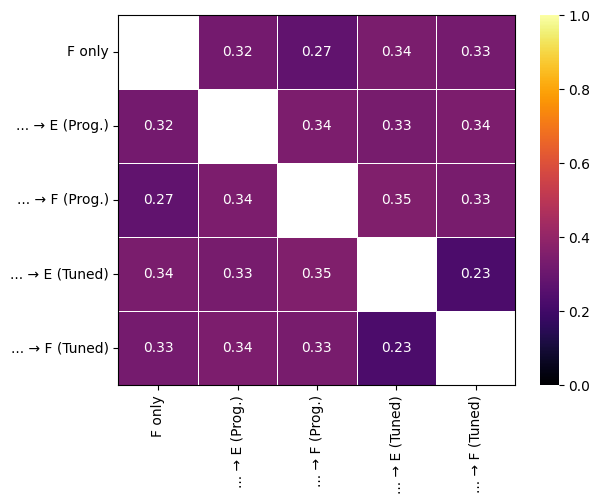
\includegraphics[width=\textwidth]{images/experiments/jsd-regf-outofdist.png}
        \caption{Regulation \textbf{F}, out-of-distribution ($n=1021$).}
        \label{fig:jsd-experiments-regf-outdist}
    \end{subfigure}
    \vskip\baselineskip
    \begin{subfigure}{.475\textwidth}
        \centering
        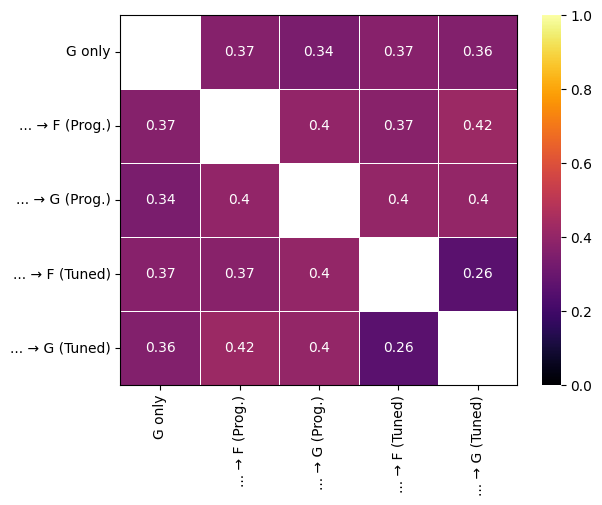
\includegraphics[width=\textwidth]{images/experiments/jsd-regg-indist.png}
        \caption{Regulation \textbf{G}, in-distribution ($n=1041$).}
        \label{fig:jsd-experiments-regg-indist}
    \end{subfigure}
    \hfill
    \begin{subfigure}{.475\textwidth}
        \centering
        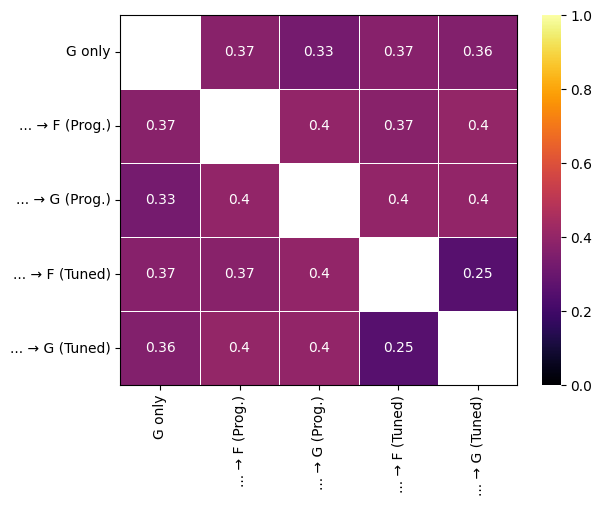
\includegraphics[width=\textwidth]{images/experiments/jsd-regg-outofdist.png}
        \caption{Regulation \textbf{G}, out-of-distribution ($n=1012$).}
        \label{fig:jsd-experiments-regg-outdist}
    \end{subfigure}
    \caption{Mean pairwise Jensen-Shannon distance between action probabilities for every observation. Letters represent the regulation the agent is trained or fine-tuned on (e.g. ``$... \rightarrow \text{F}$" is fine-tuned from regulation \textbf{A} to \textbf{B} to ... to \textbf{F}). \textit{``Prog."} refers to progressive agents.}
    \label{fig:jsd-experiments}
\end{figure}

In the next experiment we compare the value predictions of the agents when given the same observation.
The results for this experiment, plotted against the normalized depth of the observation (how many turns into the battle it was recorded), are shown in Figure \ref{fig:value-experiments}.

\begin{figure}[H]
    \centering
    \begin{subfigure}{.5\textwidth}
        \centering
        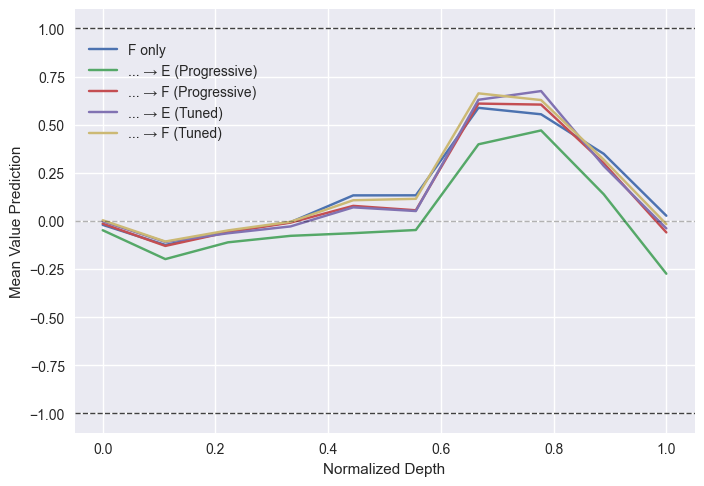
\includegraphics[width=\textwidth]{images/experiments/value-regf-indist.png}
        \caption{Regulation \textbf{F}, in-distribution ($n=924$).}
        \label{fig:value-experiments-regf-indist}
    \end{subfigure}%
    \begin{subfigure}{.5\textwidth}
        \centering
        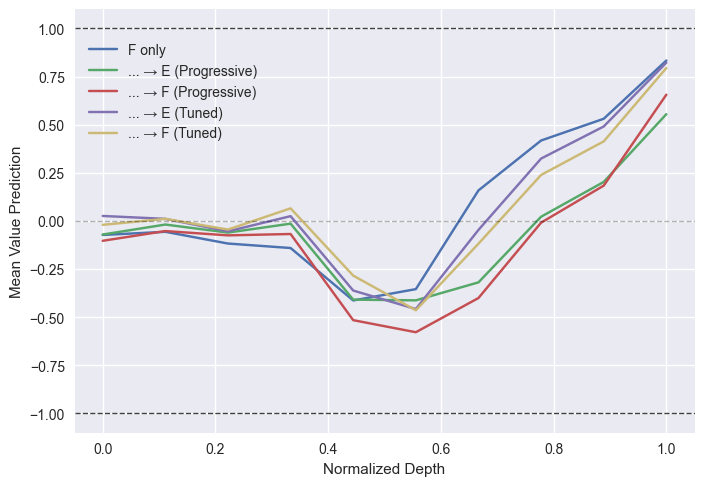
\includegraphics[width=\textwidth]{images/experiments/value-regf-outofdist.png}
        \caption{Regulation \textbf{F}, out-of-distribution ($n=1021$).}
        \label{fig:value-experiments-regf-outdist}
    \end{subfigure}
    \vskip\baselineskip
    \begin{subfigure}{.5\textwidth}
        \centering
        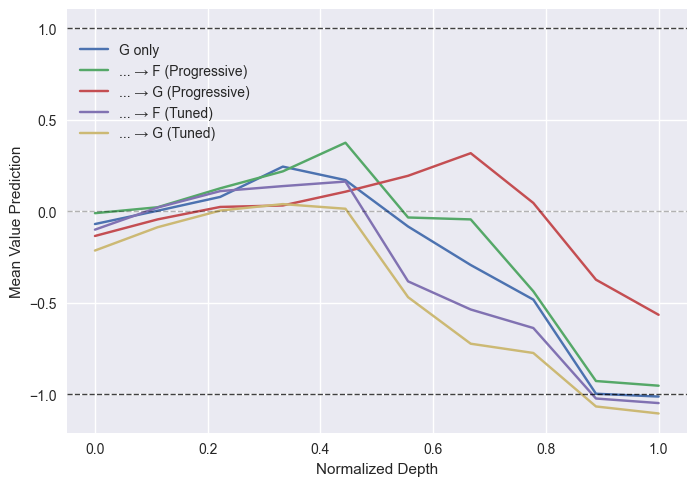
\includegraphics[width=\textwidth]{images/experiments/value-regg-indist.png}
        \caption{Regulation \textbf{G}, in-distribution ($n=1041$).}
        \label{fig:value-experiments-regg-indist}
    \end{subfigure}%
    \begin{subfigure}{.5\textwidth}
        \centering
        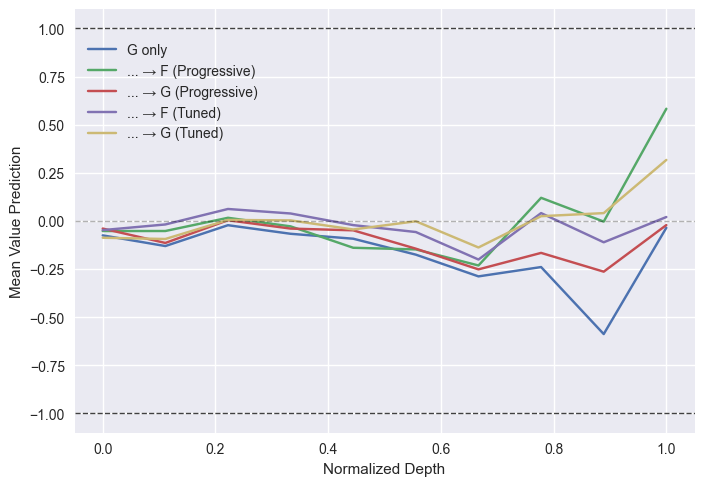
\includegraphics[width=\textwidth]{images/experiments/value-regg-outofdist.png}
        \caption{Regulation \textbf{G}, out-of-distribution ($n=1012$).}
        \label{fig:value-experiments-regg-outdist}
    \end{subfigure}
    \caption{Mean value prediction for every observation, plotted against the normalized depth. Letters represent the regulation the agent is trained or fine-tuned on (e.g. ``$... \rightarrow \text{F}$" is fine-tuned from regulation \textbf{A} to \textbf{B} to ... to \textbf{F}).}
    \label{fig:value-experiments}
\end{figure}

The last experiment involves plotting the distribution of action logits using a t-SNE visualization.
Just as in Chapter \ref{sec:preliminary:analysis}, we take the 256-dimensional action logits for each observation, reduce them to 50 dimensions using principal component analysis (PCA), then reduce them to two dimensions using t-SNE.
The visualizations for progressive and tuned agents can be found in Figures \ref{fig:tsne-progressive} and \ref{fig:tsne-tuned} respectively.

To get a clearer picture of the underlying structure of the latter visualization, we sample 50 observations (150 points) and connect points showing logits of the same observation.
Since t-SNE distorts global and local distances, we color these connecting lines according to the Jensen-Shannon distance between the action probabilities of the respective observations.
This visualization can be found in Figure \ref{fig:tsne-tuned-lines}.

\begin{figure}[ht]
    \centering
    \begin{subfigure}{.5\textwidth}
        \centering
        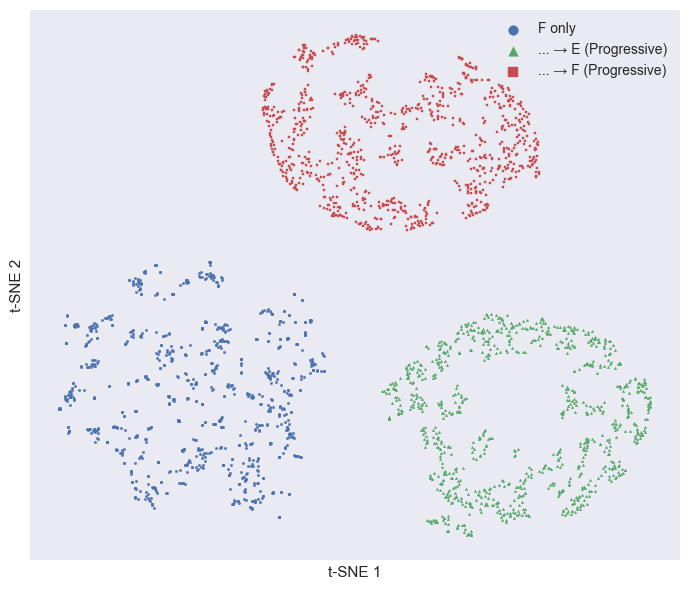
\includegraphics[width=\textwidth]{images/experiments/progressive-tsne-regf-indist.png}
        \caption{Regulation \textbf{F}, in-distribution ($n=924$).}
        \label{fig:tsne-progressive-regf-indist}
    \end{subfigure}%
    \begin{subfigure}{.5\textwidth}
        \centering
        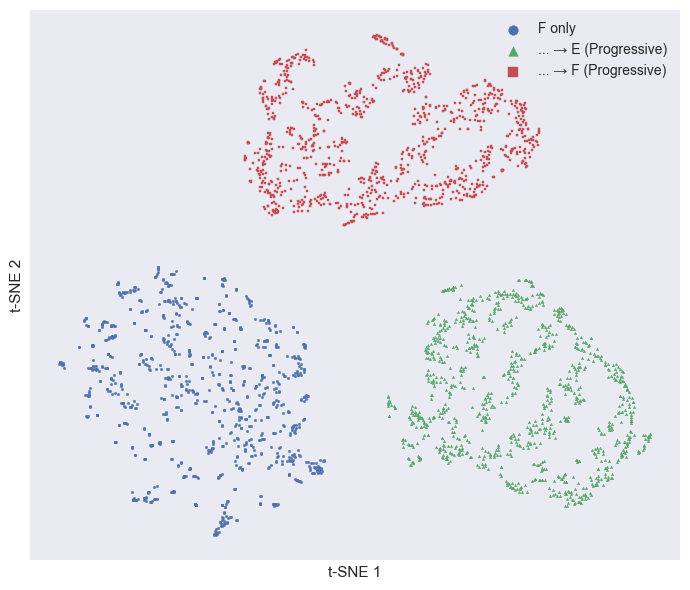
\includegraphics[width=\textwidth]{images/experiments/progressive-tsne-regf-outofdist.png}
        \caption{Regulation \textbf{F}, out-of-distribution ($n=1021$).}
        \label{fig:tsne-progressive-regf-outdist}
    \end{subfigure}
    \vskip\baselineskip
    \begin{subfigure}{.5\textwidth}
        \centering
        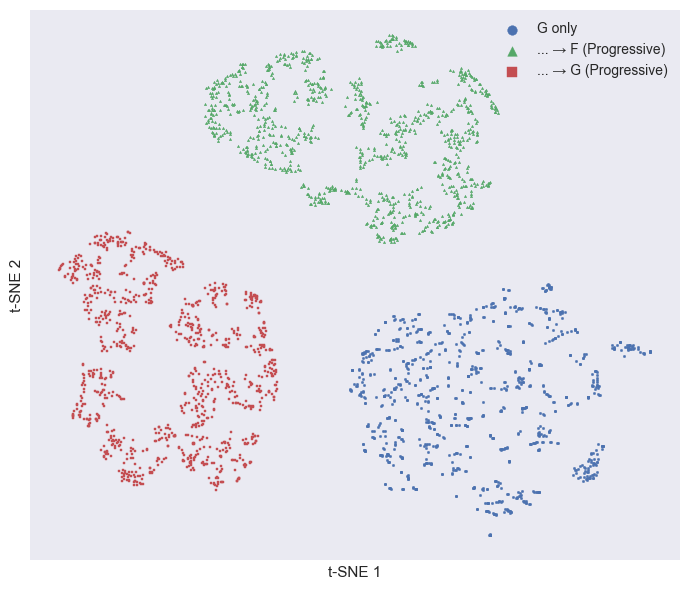
\includegraphics[width=\textwidth]{images/experiments/progressive-tsne-regg-indist.png}
        \caption{Regulation \textbf{G}, in-distribution ($n=1041$).}
        \label{fig:tsne-progressive-regg-indist}
    \end{subfigure}%
    \begin{subfigure}{.5\textwidth}
        \centering
        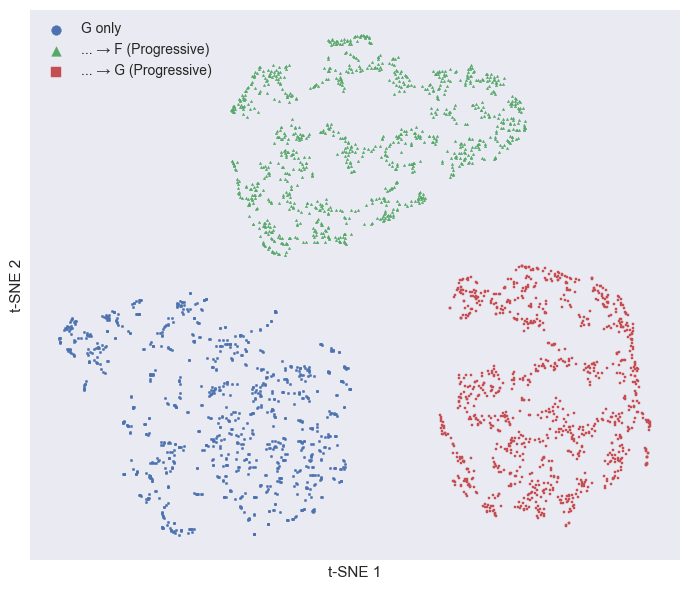
\includegraphics[width=\textwidth]{images/experiments/progressive-tsne-regg-outofdist.png}
        \caption{Regulation \textbf{G}, out-of-distribution ($n=1012$).}
        \label{fig:tsne-progressive-regg-outdist}
    \end{subfigure}
    \caption{t-SNE visualization of action logits of progressive agents for every observation. Letters represent the regulation the agent is trained or fine-tuned on (e.g. ``$... \rightarrow \text{F}$" is fine-tuned from regulation \textbf{A} to \textbf{B} to ... to \textbf{F}).}
    \label{fig:tsne-progressive}
\end{figure}

\begin{figure}[ht]
    \centering
    \begin{subfigure}{.5\textwidth}
        \centering
        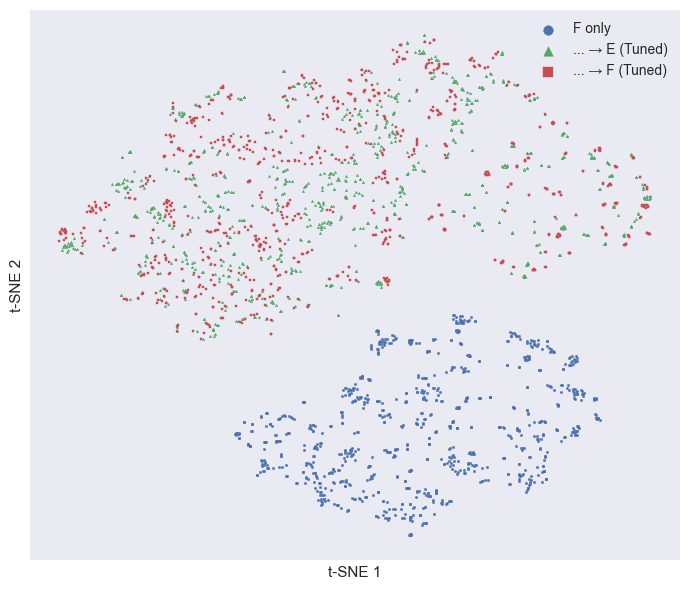
\includegraphics[width=\textwidth]{images/experiments/tuned-tsne-regf-indist.png}
        \caption{Regulation \textbf{F}, in-distribution ($n=924$).}
        \label{fig:tsne-tuned-regf-indist}
    \end{subfigure}%
    \begin{subfigure}{.5\textwidth}
        \centering
        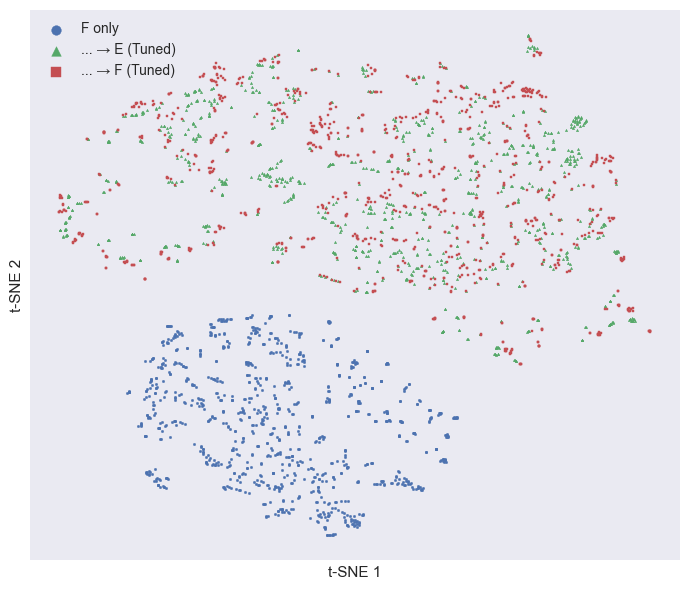
\includegraphics[width=\textwidth]{images/experiments/tuned-tsne-regf-outofdist.png}
        \caption{Regulation \textbf{F}, out-of-distribution ($n=1021$).}
        \label{fig:tsne-tuned-regf-outdist}
    \end{subfigure}
    \vskip\baselineskip
    \begin{subfigure}{.5\textwidth}
        \centering
        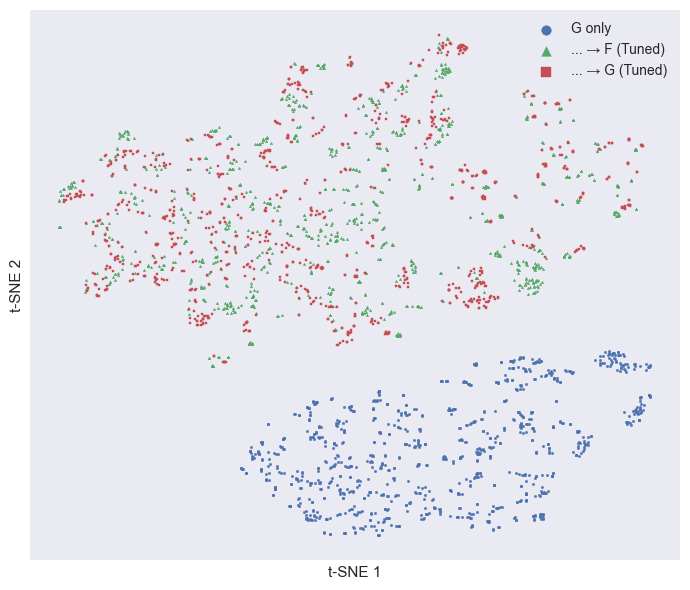
\includegraphics[width=\textwidth]{images/experiments/tuned-tsne-regg-indist.png}
        \caption{Regulation \textbf{G}, in-distribution ($n=1041$).}
        \label{fig:tsne-tuned-regg-indist}
    \end{subfigure}%
    \begin{subfigure}{.5\textwidth}
        \centering
        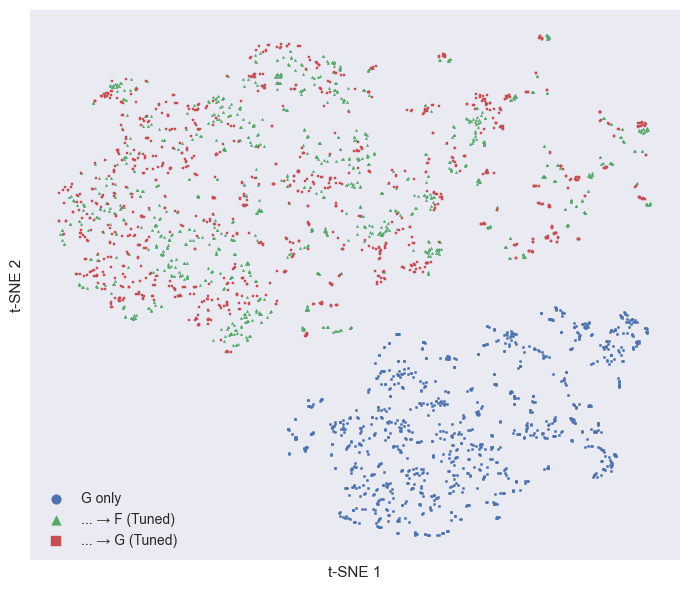
\includegraphics[width=\textwidth]{images/experiments/tuned-tsne-regg-outofdist.png}
        \caption{Regulation \textbf{G}, out-of-distribution ($n=1012$).}
        \label{fig:tsne-tuned-regg-outdist}
    \end{subfigure}
    \caption{t-SNE visualization of action logits of tuned agents for every observation. Letters represent the regulation the agent is trained or fine-tuned on (e.g. ``$... \rightarrow \text{F}$" is fine-tuned from regulation \textbf{A} to \textbf{B} to ... to \textbf{F}).}
    \label{fig:tsne-tuned}
\end{figure}

\begin{figure}[ht]
    \centering
    \begin{subfigure}{.5\textwidth}
        \centering
        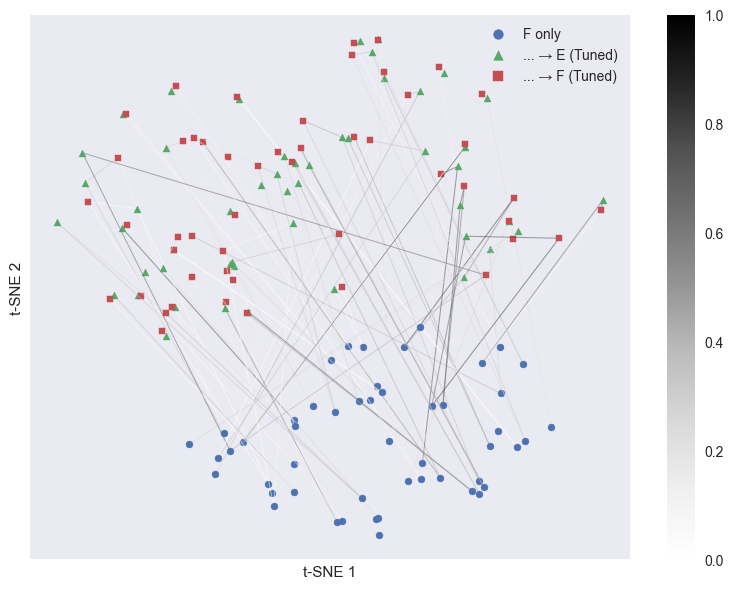
\includegraphics[width=\textwidth]{images/experiments/tuned-tsne-regf-indist-lines.png}
        \caption{Regulation \textbf{F}, in-distribution ($n=924$).}
        \label{fig:tsne-tuned-lines-regf-indist}
    \end{subfigure}%
    \begin{subfigure}{.5\textwidth}
        \centering
        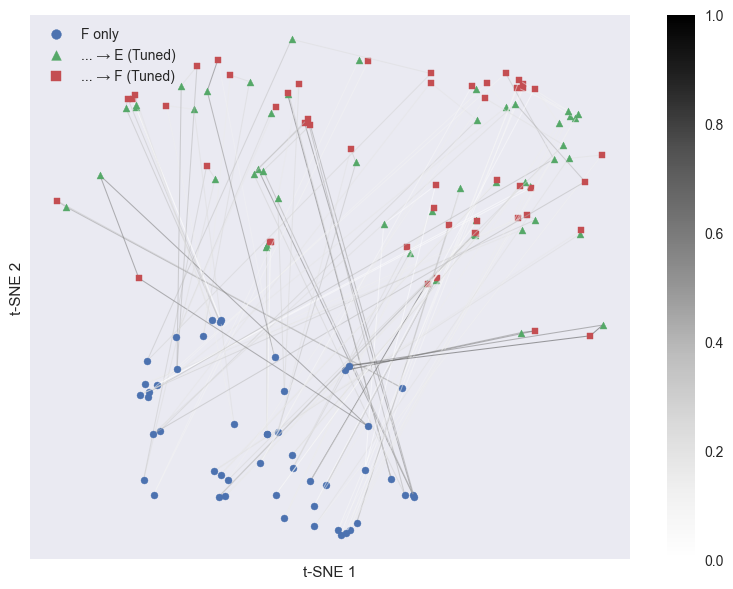
\includegraphics[width=\textwidth]{images/experiments/tuned-tsne-regf-outofdist-lines.png}
        \caption{Regulation \textbf{F}, out-of-distribution ($n=1021$).}
        \label{fig:tsne-tuned-lines-regf-outdist}
    \end{subfigure}
    \vskip\baselineskip
    \begin{subfigure}{.5\textwidth}
        \centering
        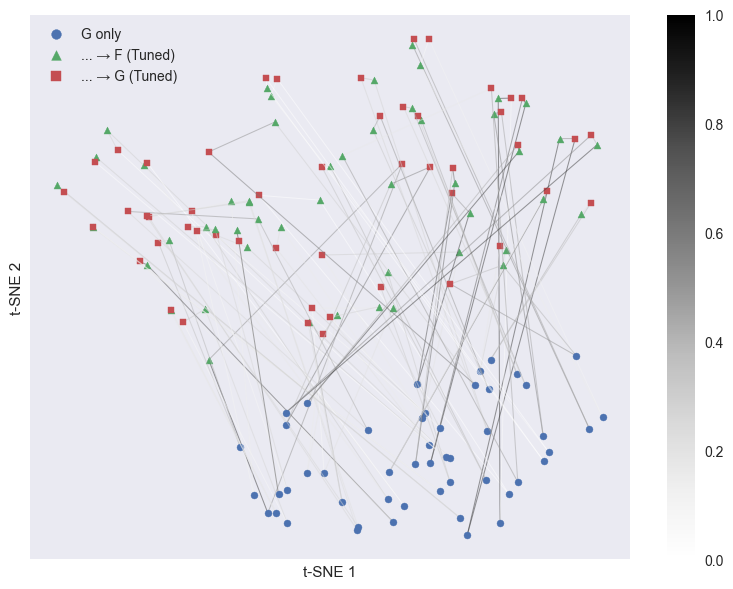
\includegraphics[width=\textwidth]{images/experiments/tuned-tsne-regg-indist-lines.png}
        \caption{Regulation \textbf{G}, in-distribution ($n=1041$).}
        \label{fig:tsne-tuned-lines-regg-indist}
    \end{subfigure}%
    \begin{subfigure}{.5\textwidth}
        \centering
        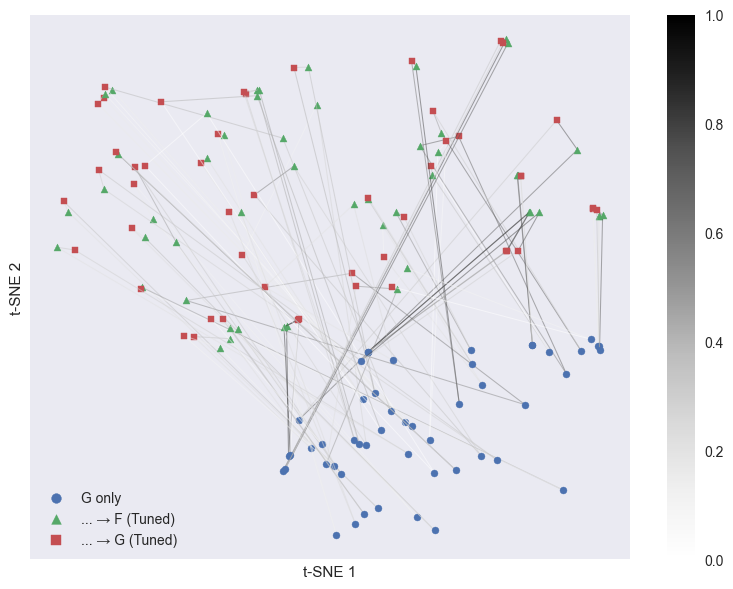
\includegraphics[width=\textwidth]{images/experiments/tuned-tsne-regg-outofdist-lines.png}
        \caption{Regulation \textbf{G}, out-of-distribution ($n=1012$).}
        \label{fig:tsne-tuned-lines-regg-outdist}
    \end{subfigure}
    \caption{t-SNE visualization of action logits of tuned agents for 50 sampled observations. Letters represent the regulation the agent is trained or fine-tuned on (e.g. ``$... \rightarrow \text{F}$" is fine-tuned from regulation \textbf{A} to \textbf{B} to ... to \textbf{F}). Lines connect points showing the same observation, and are colored according to the Jensen-Shannon distance between the respective action probabilities.}
    \label{fig:tsne-tuned-lines}
\end{figure}

\newpage
%
% Discussion
%
\chapter{Discussion} \label{sec:discussion}
In this Chapter we will discuss the results presented in Chapter \ref{sec:experiments}.

\section{Stationary Results} \label{sec:discussion:stationary}
Starting with the stationary results shown in Chapter \ref{sec:results:stationary}, we can see in Figures \ref{fig:stationary} and \ref{fig:stationary-pvalues} how the progressive and tuned agents match up against VGC-Bench's original RL agents in a stationary environment.

Since the progressive architecture only comes into play when training across multiple regulations, the results from the progressive agents only show the impact of the network adjustments we proposed with regards to the stability of the value function, outlined at the beginning of Chapter \ref{sec:methodology}.
The results show that these network adjustments appear to be a success, as the progressive agents consistently outperform the original agents, both in-distribution and out-of-distribution.
Figure \ref{fig:stationary-pvalues} shows that these results are statistically significant, with the exception of regulations \textbf{G} (in-distribution), \textbf{A}, and \textbf{I} (out-of-distribution).

Looking at the results of the tuned agents, it appears that they are also able to consistently beat the original agents, though we can see in Figure \ref{fig:stationary-pvalues} that half of the in-distribution results are not statistically significant.
It also appears that the tuned agents perform slightly worse than the progressive agents, though most of these reciprocal results are also not statistically significant.
We speculate that this may be due to tuned PPO having smaller parameter updates, leading to more underfitted models compared to regular PPO, but we do not have enough evidence to conclude this.
When evaluated out-of-distribution, the results flip and the tuned agents outperform both the original and the progressive agents in all regulations, though the latter results are not statistically significant.

We do have to acknowledge that these experiments are only performed using one seed, and may therefore show further variance when repeated on different seeds.
Taking this into account, we can tentatively conclude that our proposed network improvements lead to better agents in stationary environments.
Tuned agents achieve marginally worse results than agents trained using normal PPO, but in turn show marginally better generalization to unseen teams.

\section{Non-Stationary Results} \label{sec:discussion:nonstationary}
We now move to the non-stationary results shown in Chapter \ref{sec:results:nonstationary}, which show how progressive, tuned, and combined agents compare to the original fine-tuned and fully retrained agents.

Starting with the progressive agents, we can see in Figures \ref{fig:progressive-experiments} and \ref{fig:progressive-pvalues} that the results are quite disappointing.
The progressive agents are unable to achieve any statistically significant in-distribution result against the original fine-tuned agents or progressive agents trained from scratch.
Out-of-distribution, the progressive agents appear to be able to beat the original fine-tuned and retrained agents from time to time, but they still fail to get any statistically significant result against progressive agents trained from scratch.

Moving on to the tuned agents, we can see in Figures \ref{fig:tuned-experiments} and \ref{fig:tuned-pvalues} that these agents appear to achieve slightly better results.
The tuned agents are able to beat the original fine-tuned and retrained agents in most regulations, both in-distribution and out-of-distribution, and we can see in Figure \ref{fig:tuned-pvalues} that these results are statistically significant most of the time, especially in the latter half of regulations.
However, most of the time, we also see that the tuned agents are not significantly better than tuned agents trained from scratch.

Lastly, we can see in Figures \ref{fig:combined-experiments} and \ref{fig:combined-pvalues} that the combined agents appear to achieve slightly more promising results than the progressive agents, but not as good as the tuned agents.
In-distribution, the combined agents are sometimes able to achieve a statistically significant result against the original agents, but are clearly worse than progressive or tuned agents trained from scratch.
Out-of-distribution, the combined agents can significantly outperform the original fine-tuned and retrained agents most of the time, but they still fall short of the retrained progressive and tuned agents.

In Figure \ref{fig:compared-experiments} we compare the progressive, tuned, and combined agents directly to each other in each regulation.
These results appear similar to what we have already seen in the other experiments: The progressive agents consistently perform the worst, followed by the combined and tuned agents respectively.
In-distribution, the tuned agents are clearly superior in most regulations, beating the other agents with statistical significance in all but regulations \textbf{G} and \textbf{I}.
Out-of-distribution, the results are more varied and mostly statistically insignificant, suggesting the agents are capable of similar generalization.

We again have to acknowledge that these experiments are only performed using one seed.
Taking this into account, we tentatively conclude that our proposed progressive architecture is unable to improve the performance of VGC-Bench's RL agents in a non-stationary setting.
Agents trained and fine-tuned using tuned PPO are capable of beating fine-tuned or retrained VGC-Bench agents, but cannot consistently beat tuned agents trained from scratch.
Combining a progressive architecture with tuned PPO performs slightly better than a progressive architecture alone, but still worse than tuned PPO alone.
Finally, all of the progressive, tuned, and combined agents achieve significantly better generalization to unseen teams than VGC-Bench's original agents.

\section{Analysis Results} \label{sec:discussion:analysis}
Lastly, we discuss the results shown in Chapter \ref{sec:results:analysis} as part of the analysis into various statistics of the progressive and tuned agents in regulations \textbf{F} and \textbf{G}.

The first experiment involves the mean pairwise distances between the agents' action probabilities, shown in Figure \ref{fig:jsd-experiments}.
Generally speaking, we can see that there is not much variation between the mean distances, but there are some notable exceptions.
In all subfigures we can see that the progressive agent fine-tuned up to the current regulation is closer in behavior to the agent trained from scratch than to its source model, highlighting how a progressive architecture inherently does not suffer from loss of plasticity.
Conversely, the tuned agents are notably closer to their source models than to the agents trained from scratch, suggesting they are still experiencing some loss of plasticity.

Figure \ref{fig:value-experiments} shows the value predictions of the agents plotted against the normalized depth.
The main thing that stands out here is that, despite the network adjustments we proposed specifically in view of the unstable value predictions in the preliminary experiments, the value predictions still show some unexpected and inconsistent behavior.
Looking back to the value predictions in the preliminary experiments, shown in Figure \ref{fig:value}, we can still draw some comparisons.

The first thing of note is that the variance between the different agents appears to have shrunk, with most lines in Figure \ref{fig:value-experiments} following near identical trajectories, especially for earlier observations.
One thing that initially stood out to us about the value predictions in the preliminary experiments is that there are moments where the mean value prediction drifts outside of the range of the reward function, $[-1,1]$.
Although we can still observe this happening in Figure \ref{fig:value-experiments-regg-indist}, the amount and fraction spent outside of the reward range has decreased compared to the preliminary experiments.
Lastly, we can observe a general trend that the mean predictions start around zero as expected, and only grow more extreme and unstable as the observations get deeper into the episode.
This trend is also visible in Figure \ref{fig:value}, but more pronounced in these more recent experiments.
All things considered, these comparisons suggest that our proposed network adjustments did have a measurable effect on the agents' value function, but that most of the unexpected and inconsistent behavior is likely caused by a broader limitation in the policy architecture, training procedure, or environment.

The last experiment involves visualizing the distribution of action logits using a t-SNE visualization, the results of which can be found in Figure \ref{fig:tsne-progressive} for the progressive agents.
Here we can clearly observe that each agents' action logits can be clearly distinguished from the other agents', again highlighting how a progressive architecture inherently does not suffer from loss of plasticity.
The t-SNE visualizations for tuned agents can be found in Figures \ref{fig:tsne-tuned} and \ref{fig:tsne-tuned-lines}.
These results look near identical to Figures \ref{fig:tsne} and \ref{fig:tsne-lines} from the preliminary experiments, suggesting that the tuned agents are still experiencing some loss of plasticity.

\newpage
%
% Conclusion
%
\chapter{Conclusion} \label{sec:conclusion}
At the beginning of this thesis we set out to address the following problem statement: ``How can we train reinforcement learning agents on competitive games that receive frequent updates, with each update possibly invalidating previously learned strategies?"
We identified continual reinforcement learning as a promising direction for addressing this problem, and investigated its potential in the domain of VGC.
Rounding up all the experiments and results, we can now reflect back and answer the three research questions posed at the start of this thesis:

\paragraph{1. What effect does non-stationarity have on the performance and generalization of reinforcement learning agents in VGC?} We showed in Chapter \ref{sec:preliminary} that reinforcement learning agents trained on one VGC regulation are consistently worse than retrained agents in other regulations, suggesting that the non-stationary input distribution caused by the different regulations seriously harms the performance of reinforcement learning agents in VGC.
When evaluating using teams that no agent has seen before, the agents are capable of matching or even beating agents trained on future regulations, suggesting that non-stationarity has less of an impact on the generalization of reinforcement learning agents in VGC.

\paragraph{2. Can continual reinforcement learning methods facilitate effective knowledge transfer across game versions?} We showed in Chapter \ref{sec:preliminary} that reinforcement learning agents can successfully transfer knowledge short-term using full fine-tuning, and we identified loss of plasticity and unstable value predictions as possible causes for degraded performance in the long term.
In Chapter \ref{sec:methodology}, we made minor network adjustments to aid with the stability of the value predictions during training, and we proposed a progressive architecture and tuned PPO as continual reinforcement learning methods potentially capable of mitigating loss of plasticity and prolonging positive transfer.
In Chapter \ref{sec:experiments}, we showed that our proposed network adjustments together with tuned PPO can outperform the original fine-tuned agents, and therefore transfer knowledge more effectively over multiple regulations.
Additionally, agents trained using this combination are consistently capable of better generalization to unseen teams.
Our proposed progressive architecture, both with and without tuned PPO, is unable to effectively transfer knowledge across regulations, but is still capable of better generalization to unseen teams than the original models.
Our proposed network adjustments are able to marginally reduce the unstable value predictions, but the retained instability suggest these are more likely caused by a broader limitation in the policy architecture, training procedure, or VGC environment.
Lastly, we showed that the progressive architecture does not suffer from loss of plasticity, while this still appears to be a possible issue for tuned PPO.

\paragraph{3. How do continual reinforcement learning-based agents compare to fully retrained agents in terms of performance, generalization, and training cost across game updates?} While the combination of our network adjustments and tuned PPO is able to outperform the original fully fine-tuned agents, it is unable to consistently outperform agents with the same combination retrained from scratch.
The same holds true with regards to generalization to unseen teams.
Since all our experiments provide an upper bound of the expected performance, we can conclude that retrained agents are superior to agents that attempt to transfer knowledge across regulations in terms of performance, generalization, and training cost.
While this means that the initial goal of knowledge transfer across regulations instead of retraining has not been not achieved, we did show that continual reinforcement learning-based agents are able to outright outperform the original agents and achieve better generalization to unseen teams, suggesting that continual reinforcement learning is still beneficial to reinforcement learning agents in VGC.
To finish our main conclusions, we have to acknowledge that the majority of experiments in this thesis were only performed on one seed, and that we observed outliers in both the positive and negative direction.
These conclusions are therefore largely tentative, and will benefit from further investigation on different seeds.

\section{Future Work} \label{sec:futurework}
Starting with our own work, we of course underline the importance of repeating our experiments on multiple seeds.
We also identify multiple loose ends that we could not fully explore due to limitations in time, resources, and the scope of our research:

\begin{itemize}
    \item The value predictions shown in Chapter \ref{sec:results:analysis} still show unstable and inconsistent behavior. Getting to the bottom of this instability could lead to valuable insights into the interaction between reinforcement learning agents and the VGC environment.
    \item We opted for a conservative L2 regularization rate of 1e-6 for tuned PPO. Seeing the promising results of this method, experimenting further with different values of this parameter is a natural next step.
    \item Similarly, we opted for always training on 64 teams seen during training because of its increased generalization. It is still unclear how agents trained on fewer (or more) teams would transfer to different regulations.
    \item We always fine-tune agents using the same hyperparameters as regular training. Seeing what tuned PPO achieves with only a few adjustments, optimizing these hyperparameters for fine-tuning could lead to significantly different results.
    \item We omitted specialized optimization methods like ReDo and Continual Backprop in favor of tuned PPO. Seeing the promising results of tuned PPO, adapting these optimization methods to our policy architecture is a natural next step.
    \item We also omitted regularization- and replay-based methods because of their focus on catastrophic forgetting, leaving it unclear what impact they could have in our problem setting.
    \item Despite the progressive architecture not showing any promising results, its inherent lack of loss of plasticity still fits our problem setting exceptionally well and is therefore still a promising approach that needs further investigation, specifically in how to effectively transfer the learned representations of smaller transformer models.
    \item We believe more insights could be gained by experimenting with custom regulations, allowing for better control over the scale of non-stationarity.
    \item Lastly, our experiments could also be repeated in other, possibly simpler, games that still see natural non-stationarity. This would help separate the complexity of continual learning from the complexity of the VGC environment.
\end{itemize}

Looking more generally at the current state of continual (reinforcement) learning, we believe continual learning in non-stationary competitive games is a severely understudied domain that shows great, unexplored potential.
Modern competitive games, like VGC, are an intuitive example of naturally evolving non-stationary environments with clearly defined rules, goals, and task boundaries.
With continual learning aiming to solve the crucial problem of allowing agents to keep learning and improving after deployment, we believe that non-stationary competitive games could serve as a natural benchmark, facilitating a greater understanding of how machine learning agents can remain effective in ever-evolving environments.


% references
\newpage
\sloppy
\printbibliography

% appendix
\newpage
%
% Appendix
%
\appendix
\chapter{Additional Figures} \label{app:figures}
\begin{figure}[ht]
    \centering
    \begin{subfigure}{.5\textwidth}
        \centering
        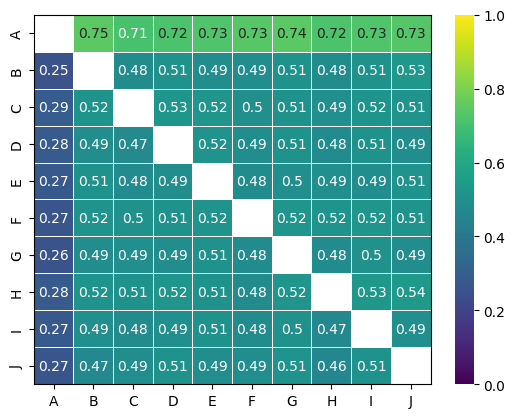
\includegraphics[width=0.8\textwidth]{images/appendix/zs-indist-a.png}
        \caption{In-distribution.}
    \end{subfigure}%
    \begin{subfigure}{.5\textwidth}
        \centering
        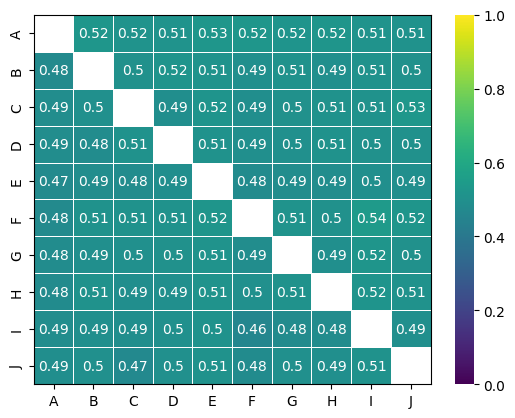
\includegraphics[width=0.8\textwidth]{images/appendix/zs-outdist-a.png}
        \caption{Out-of-distribution.}
    \end{subfigure}
    \caption{Win rates of the row player over 1000 episodes and three seeds, evaluated on regulation \textbf{A} (See Chapter \ref{sec:preliminary:transfer}).}
\end{figure}

\begin{figure}[h!]
    \centering
    \begin{subfigure}{.5\textwidth}
        \centering
        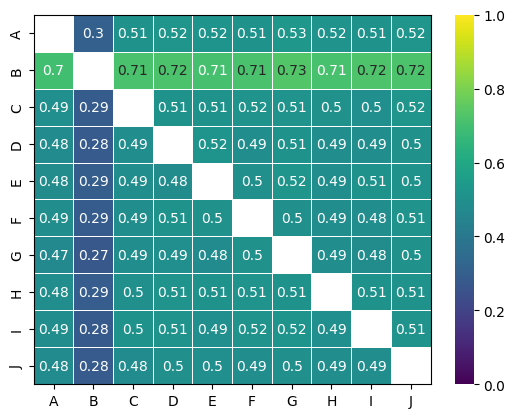
\includegraphics[width=0.8\textwidth]{images/appendix/zs-indist-b.png}
        \caption{In-distribution.}
    \end{subfigure}
    \caption{Win rates of the row player over 1000 episodes and three seeds, evaluated on regulation \textbf{B} (See Chapter \ref{sec:preliminary:transfer}).}
\end{figure}

\begin{figure}[p]
    \centering
    \begin{subfigure}{.5\textwidth}
        \centering
        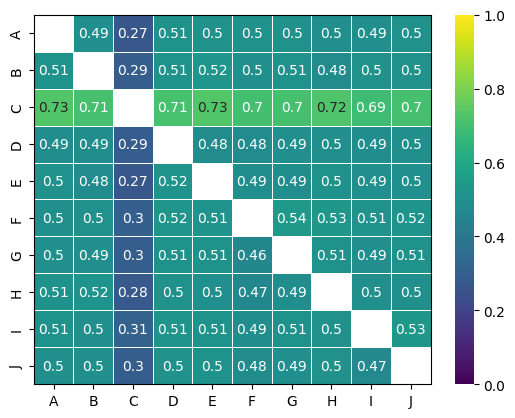
\includegraphics[width=\textwidth]{images/appendix/zs-indist-c.png}
        \caption{In-distribution.}
    \end{subfigure}%
    \begin{subfigure}{.5\textwidth}
        \centering
        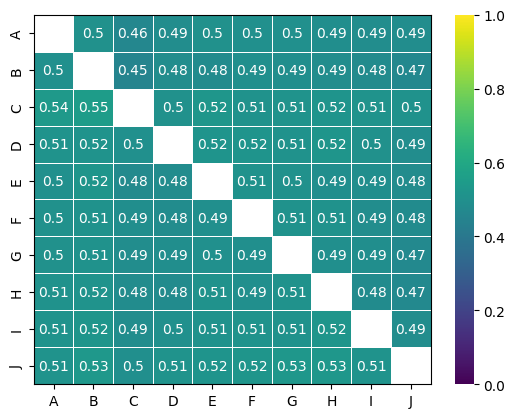
\includegraphics[width=\textwidth]{images/appendix/zs-outdist-c.png}
        \caption{Out-of-distribution.}
    \end{subfigure}
    \caption{Win rates of the row player over 1000 episodes and three seeds, evaluated on regulation \textbf{C} (See Chapter \ref{sec:preliminary:transfer}).}
\end{figure}

\begin{figure}[p]
    \centering
    \begin{subfigure}{.5\textwidth}
        \centering
        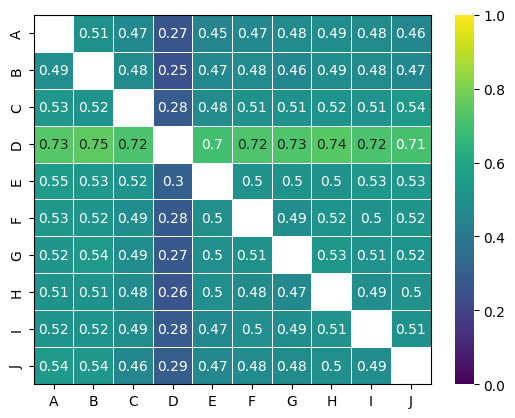
\includegraphics[width=\textwidth]{images/appendix/zs-indist-d.png}
        \caption{In-distribution.}
    \end{subfigure}%
    \begin{subfigure}{.5\textwidth}
        \centering
        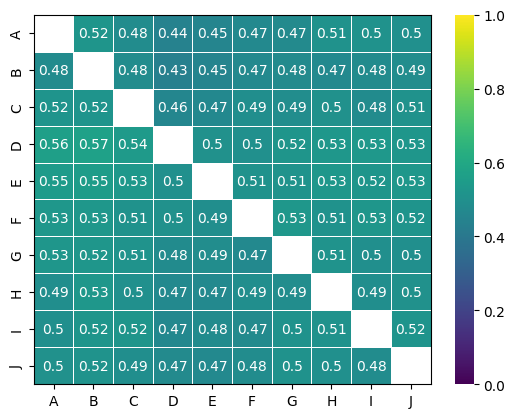
\includegraphics[width=\textwidth]{images/appendix/zs-outdist-d.png}
        \caption{Out-of-distribution.}
    \end{subfigure}
    \caption{Win rates of the row player over 1000 episodes and three seeds, evaluated on regulation \textbf{D} (See Chapter \ref{sec:preliminary:transfer}).}
\end{figure}

\begin{figure}[p]
    \centering
    \begin{subfigure}{.5\textwidth}
        \centering
        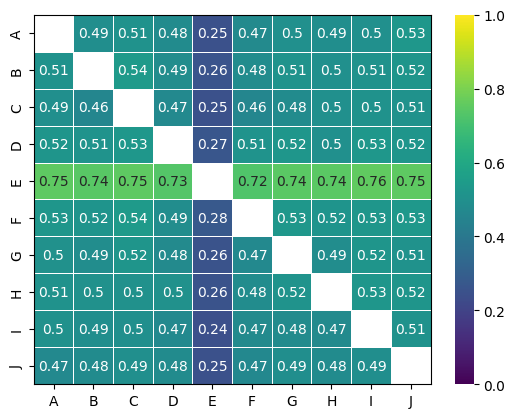
\includegraphics[width=\textwidth]{images/appendix/zs-indist-e.png}
        \caption{In-distribution.}
    \end{subfigure}
    \caption{Win rates of the row player over 1000 episodes and three seeds, evaluated on regulation \textbf{E} (See Chapter \ref{sec:preliminary:transfer}).}
\end{figure}

\begin{figure}[p]
    \centering
    \begin{subfigure}{.5\textwidth}
        \centering
        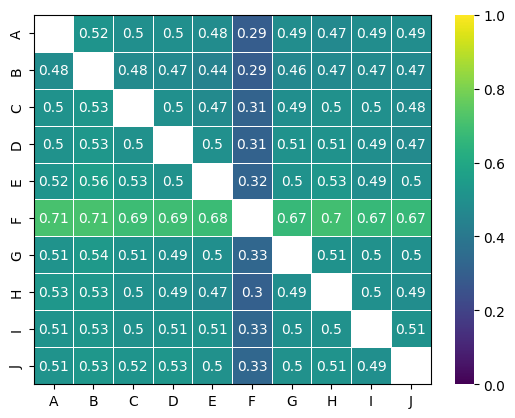
\includegraphics[width=\textwidth]{images/appendix/zs-indist-f.png}
        \caption{In-distribution.}
    \end{subfigure}%
    \begin{subfigure}{.5\textwidth}
        \centering
        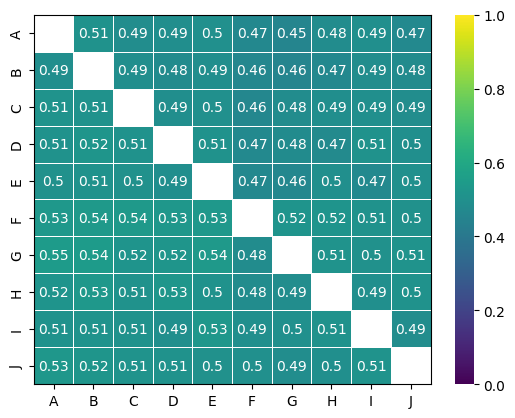
\includegraphics[width=\textwidth]{images/appendix/zs-outdist-f.png}
        \caption{Out-of-distribution.}
    \end{subfigure}
    \caption{Win rates of the row player over 1000 episodes and three seeds, evaluated on regulation \textbf{F} (See Chapter \ref{sec:preliminary:transfer}).}
\end{figure}

\begin{figure}[p]
    \centering
    \begin{subfigure}{.5\textwidth}
        \centering
        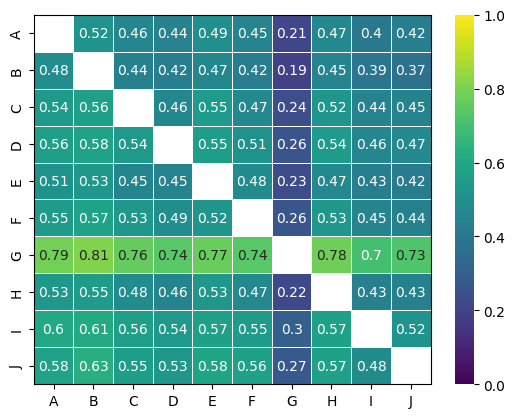
\includegraphics[width=\textwidth]{images/appendix/zs-indist-g.png}
        \caption{In-distribution.}
    \end{subfigure}%
    \begin{subfigure}{.5\textwidth}
        \centering
        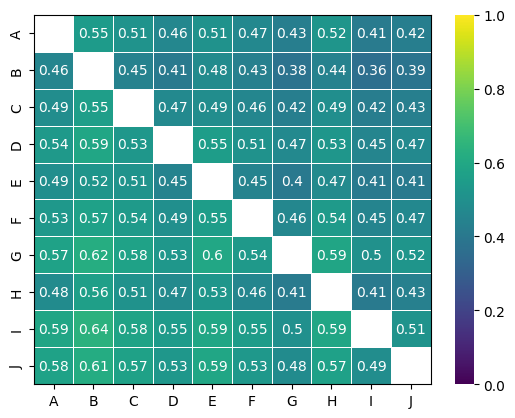
\includegraphics[width=\textwidth]{images/appendix/zs-outdist-g.png}
        \caption{Out-of-distribution.}
    \end{subfigure}
    \caption{Win rates of the row player over 1000 episodes and three seeds, evaluated on regulation \textbf{G} (See Chapter \ref{sec:preliminary:transfer}).}
\end{figure}

\begin{figure}[p]
    \centering
    \begin{subfigure}{.5\textwidth}
        \centering
        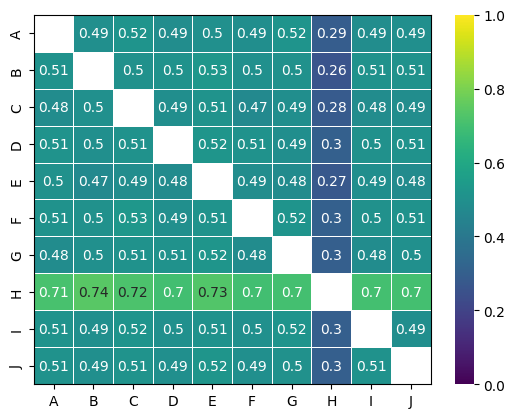
\includegraphics[width=\textwidth]{images/appendix/zs-indist-h.png}
        \caption{In-distribution.}
    \end{subfigure}%
    \begin{subfigure}{.5\textwidth}
        \centering
        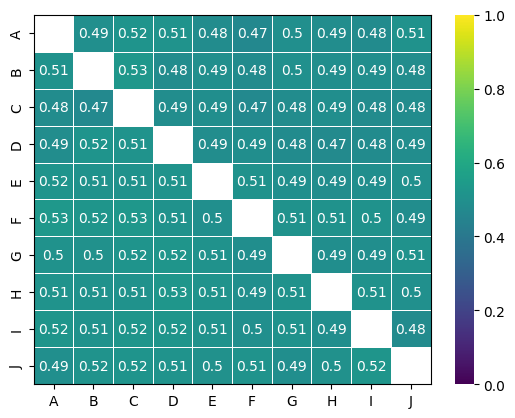
\includegraphics[width=\textwidth]{images/appendix/zs-outdist-h.png}
        \caption{Out-of-distribution.}
    \end{subfigure}
    \caption{Win rates of the row player over 1000 episodes and three seeds, evaluated on regulation \textbf{H} (See Chapter \ref{sec:preliminary:transfer}).}
\end{figure}

\begin{figure}[p]
    \centering
    \begin{subfigure}{.5\textwidth}
        \centering
        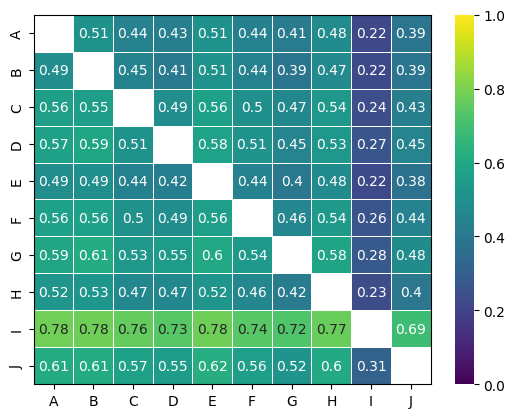
\includegraphics[width=\textwidth]{images/appendix/zs-indist-i.png}
        \caption{In-distribution.}
    \end{subfigure}%
    \begin{subfigure}{.5\textwidth}
        \centering
        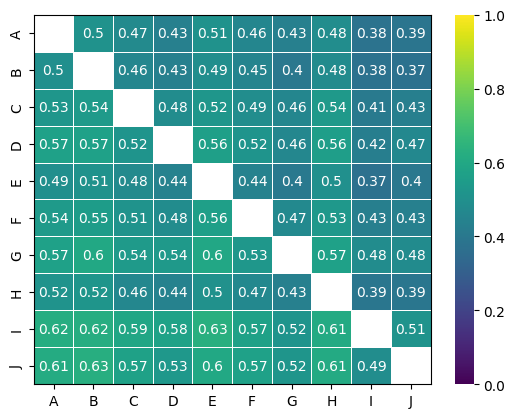
\includegraphics[width=\textwidth]{images/appendix/zs-outdist-i.png}
        \caption{Out-of-distribution.}
    \end{subfigure}
    \caption{Win rates of the row player over 1000 episodes and three seeds, evaluated on regulation \textbf{I} (See Chapter \ref{sec:preliminary:transfer}).}
\end{figure}

\begin{figure}[p]
    \centering
    \begin{subfigure}{.5\textwidth}
        \centering
        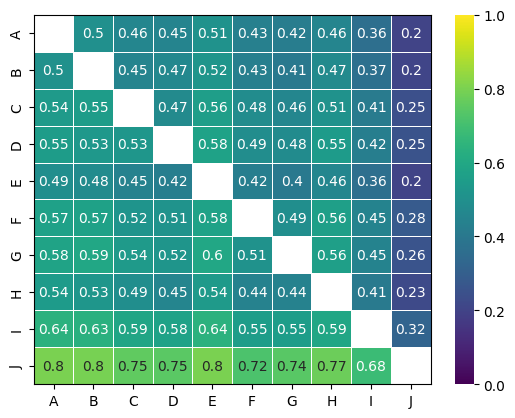
\includegraphics[width=\textwidth]{images/appendix/zs-indist-j.png}
        \caption{In-distribution.}
    \end{subfigure}
    \caption{Win rates of the row player over 1000 episodes and three seeds, evaluated on regulation \textbf{J} (See Chapter \ref{sec:preliminary:transfer}).}
\end{figure}

\begin{figure}[p]
    \centering
    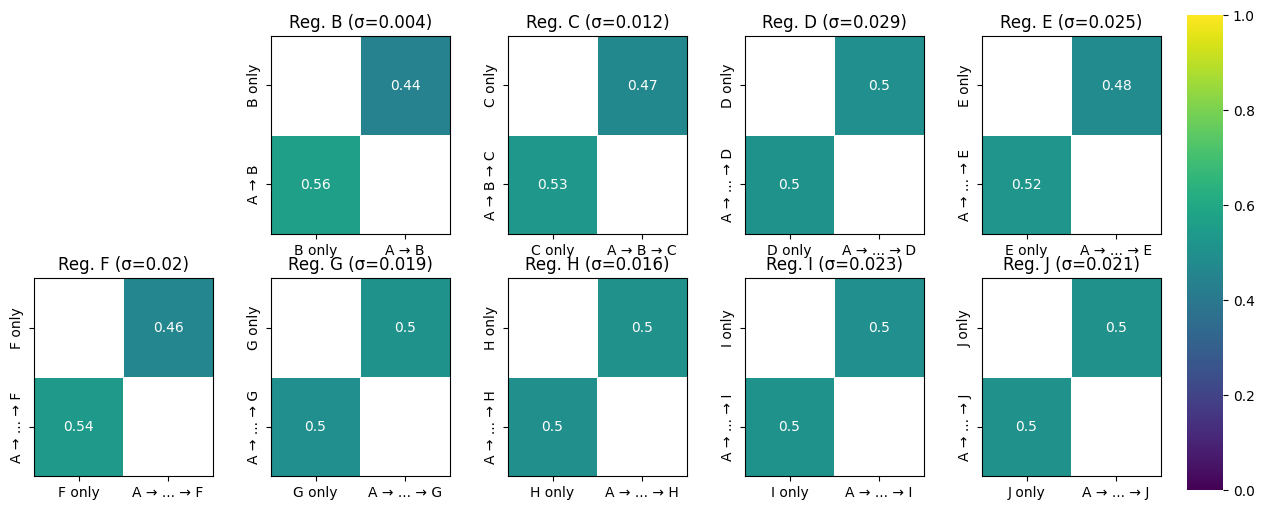
\includegraphics[width=\textwidth]{images/appendix/ft-indist.png}
    \caption{Mean win rates of fine-tuned agents against agents trained from scratch. Evaluated in-distribution over 1000 episodes and three seeds on each regulation (See Chapter \ref{sec:preliminary:finetune}).}
\end{figure}

\begin{figure}[p]
    \centering
    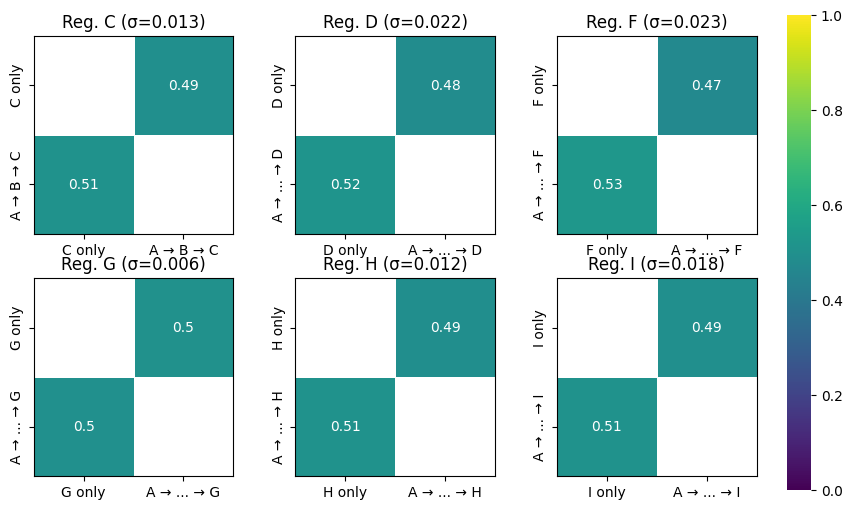
\includegraphics[width=\textwidth]{images/appendix/ft-outofdist.png}
    \caption{Mean win rates of fine-tuned agents against agents trained from scratch. Evaluated out-of-distribution over 1000 episodes and three seeds on each regulation (See Chapter \ref{sec:preliminary:finetune}).}
\end{figure}


\end{document}
